\documentclass{EPL-master-thesis-covers-EN}

\usepackage{hyperref}
\usepackage{setspace}
\usepackage[table]{xcolor}
\usepackage{tikz}
\usepackage{array}
\usepackage{tabularx}
\usepackage{longtable}
\usepackage{amsmath}
\usepackage{amssymb}
\usepackage{subcaption}
\usepackage{float}
\usepackage{pgfplots}
\pgfplotsset{compat=1.18}
\usetikzlibrary{positioning,arrows.meta,calc,shapes,fit}
\newcolumntype{P}[1]{>{\raggedright\arraybackslash}p{#1}}
\newcolumntype{Y}{>{\raggedright\arraybackslash}X}

\usepackage{csquotes}
\usepackage[style=apa,backend=biber]{biblatex}
\addbibresource{references.bib}

\geometry{margin=2.8cm}
\onehalfspacing

% Metadata for the title page
\title{PhenoHive}
\subtitle{An intuitive, modular and low-cost phenotyping station}
\author{Adrien \textsc{Montariol}}
\degreetitle{Master [120] in Computer Science}
\supervisor{Cristel \textsc{Pelsser}}
\secondsupervisor{Laurent \textsc{Francis}}
\readerone{Xavier \textsc{Draye}}
\readertwo{Sebastien \textsc{Toussaint}}
\years{2025--2026}

\begin{document}

\maketitle
\restoregeometry

\pagenumbering{roman}

\chapter*{Abstract}
\addcontentsline{toc}{chapter}{Abstract}

PhenoHive is a portable, low-cost station that monitors a single plant continuously. It runs in the LBIR1251 plant biology course at UCLouvain, where about 20 student groups carry out month-long experiments in parallel, most of them in their own homes rather than a controlled lab. A teaching platform like this has to satisfy two demands at once: the sensor data must be accurate enough to interpret in physiological terms, and the hardware has to keep running unattended for weeks. The version I inherited fell short on three fronts. Its codebase was monolithic, so extending or maintaining it was awkward. The sensors were too basic and hadn't been validated against references, which left derived quantities such as vapor pressure deficit and spectral band assignments impossible to trust. And it coped badly with the network and power interruptions that are routine in a home.

In order to fill the gap in measurements, I calibrated the environmental and light sensors in a controlled laboratory. These corrections drop the uncertainty on measurements down to a level that allows the students to be confident in the data and will allow them to interpret the measurements in physiological terms. To achieve this, I characterized the light spectrum across all of it's channels by using a monochromator and I calibrated the environmental sensor by using a controlled chamber. The deployment also changed how the station stores and pushes data to the server. It now always writes each measurement locally first in order to not lose any data during potential network outages. Students can also connect the device to their WiFi network through a captive portal instead of a terminal, remote management runs over a private network overlay and every team's dashboard is automatically created the first time their station is connected to the server. My testing on physical hadware validated three critical things. First that a fresh station can start pushing live data to the server within five minutes. Second it that a long disconnection from the server doesn't create any data loss. And third is that a student's data is never accessible to another student from another group. 


\chapter*{Acknowledgements}
\addcontentsline{toc}{chapter}{Acknowledgements}
My first thanks go to my supervisors, Cristel Pelsser and Laurent Francis, for their guidance and support throughout this project. Cristel set up the UCLouvain server infrastructure and stayed available all year, both of which were essential to finishing this thesis. Laurent's expertise in sensor methodology and calibration kept the hardware work grounded in sound metrological practice.

Xavier Draye also helped me beyond just reading the final manuscript. As the professor for the LBIR1251 course, he helped me work out what were the requirements for this iteration of the project. So what to improve, what was already fine and which physiological metrics mattered. These conversations helped establish the scope of the project and kept it focused on the things that would make a difference for the students. I am grateful for his time and insights on this matter as well as for his reading of the final manuscript.

Thanks to Sebastien Toussaint for agreeing to sit on my jury and for taking the time to review this work.

Tom Klauner at the WELCOME lab helped me through the sensor calibration sessions and was generous with his time throughout that process, for which I am very grateful.

Alexandre and Arnaud Wery helped me in designing the 3D-printed casing and soldering the station's components. I therefore want to thank them both. 

Finally, I want to thank my family: my mother Virginie Goffaux, my father Eric Montariol, and Colin Larcombe, for their careful proofreading and for their support throughout this year.



\tableofcontents
\listoffigures
\listoftables

\chapter*{List of Abbreviations}
\addcontentsline{toc}{chapter}{List of Abbreviations}
\renewcommand{\arraystretch}{1.25}
\begin{tabular}{@{}lp{4.8cm}@{\hspace{0.4cm}}lp{4.8cm}@{}}
\textbf{ADC}    & Analog-to-Digital Converter          & \textbf{MAD}   & Median Absolute Deviation \\
\textbf{BCM}    & Broadcom GPIO numbering scheme       & \textbf{NAT}   & Network Address Translation \\
\textbf{CIE}    & Commission Internationale de l'Éclairage & \textbf{NDIR} & Non-Dispersive Infrared \\
\textbf{CSI}    & Camera Serial Interface              & \textbf{NIR}   & Near-Infrared \\
\textbf{CV}     & Coefficient of Variation             & \textbf{PAR}   & Photosynthetically Active Radiation \\
\textbf{EPL}    & École Polytechnique de Louvain       & \textbf{RH}    & Relative Humidity \\
\textbf{FDM}    & Fused Deposition Modelling           & \textbf{RPi}   & Raspberry Pi \\
\textbf{GDPR}   & General Data Protection Regulation   & \textbf{SBC}   & Single-Board Computer \\
\textbf{I$^2$C} & Inter-Integrated Circuit             & \textbf{SSID}  & Service Set Identifier \\
\textbf{IaC}    & Infrastructure as Code               & \textbf{TA}    & Teaching Assistant \\
\textbf{ISP}    & Image Signal Processor               & \textbf{TSDB}  & Time-Series Database \\
\textbf{JSONL}  & JSON Lines (newline-delimited JSON)  & \textbf{UFW}   & Uncomplicated Firewall \\
\textbf{TSM}    & Time-Structured Merge-tree (InfluxDB) & \textbf{VPD}   & Vapor Pressure Deficit \\
\textbf{TSI}    & Time Series Index (InfluxDB)         & \textbf{WELCOME} & Wallonia Electronics and Communications Measurements \\
\end{tabular}
\renewcommand{\arraystretch}{1}



\clearpage
\pagenumbering{arabic}

% ── Main chapters ──────────────────────────────────────────────────────────────
\chapter{Introduction}
\label{ch:introduction}

\begingroup
\setlength{\parskip}{0.6em}

PhenoHive is a portable phenotyping station built for LBIR1251, the plant biology and physiology course at UCLouvain. One of the things that course tries to do is tie physiological theory to hands-on observation, across topics like water balance, mineral nutrition, photosynthesis and how plants respond to their environment. Traditionally that has meant shared greenhouse space and measurements taken by hand, which caps how much and how freely students can experiment.

Because of the fact that each unit is small enough and is able to run on its own, watching a single plant for weeks and producing data students can relate back to what they see in class. All without the need for a greenhouse or lab bench. A group can design its own experiment, change the conditions, and watch the effects play out close to real time. The limits that are traditionally set by the need to share space and instruments with a large group are lifted. This allows the course to be more flexible, and for students to be more creative than what was previously possible.


I came to this project from a long interest in embedded systems, and in how hardware and software actually behave in a real world environment. PhenoHive encompasses a large amount of the computer science curriculum into one place: low-level sensor communication, software structure, data persistence, networked services, visualising results, and keeping all of it alive in the field. The breadth is what made it hard. It is also what made it worth doing.

\textcite{goffinet2024} moved the OS to DietPi \parencite{dietpi}, added a rolling-median filter for the mass readings, and wrote an automated first-boot routine that bootstrapped a local InfluxDB/Grafana instance straight from a preconfigured SD card, showing that a station based on the Raspberry Pi Zero W could run on its own in a teaching setting. \textcite{colinet2025} took that further. The hardware moved from the Zero W to the faster Zero 2W. The PlantCV pipeline was brought up to version 4.6 with automatic calibration and shadow detection, and the InfluxDB/Grafana stack was relocated from a local RPi hotspot to a shared UCLouvain server. Colinet also added a resistive soil-moisture probe read through an MCP3008 ADC and a photoresistor for ambient light, and replaced the enclosure with a compact 3D-printed design.
\newline By the time I started, the station already worked end to end: it brought up its hardware, took and timestamped measurements, and pushed them to a central dashboard.

Even so, the prototype I inherited had real limitations for sustained classroom use. The software was heavily monolithic, which made it hard to maintain or extend. Measurement quality was uneven too. Mass tracking was solid enough for evapotranspiration work, and the PlantCV camera pipeline \parencite{gehan2017plantcv, plantcv} gave detailed growth indicators, but the air and light sensors were not good enough for any deeper physiological reading. The resistive soil-moisture probe returned a single index with no connection to the atmospheric water-vapor status that a vapor pressure deficit calculation needs. The photoresistor collapsed all incoming light into one lux-like number, so it could not separate the red and far-red bands that drive phytochrome-mediated development. And the platform tended to falter during the long, multi-group home deployments where dropped networks and failing instruments are simply part of normal operation.

My goal was to turn this working prototype into a platform that could be maintained and extended over time. I did not start over. Instead I kept and built on the parts that already worked, and reworked the parts that plainly did not.

The work pursues three objectives.

The first is architectural. The runtime is broken out of its monolithic form into modular components, each responsible for one concern: acquisition, processing, persistence, visualization, and the user interface. Splitting things up this way lowers the maintenance burden and makes it less likely that a teaching assistant (TA) extending the platform will break something elsewhere.

The second concerns sensing quality. Choosing better sensors isn't enough. They have to be calibrated and validated against references. This is why I calibrated the temperature and humidity sensor in a controlled chamber, and characterized the light spectrum with a monochromator. This allows the students to be confident in the data and to interpret it in physiological terms, which is what the course is about.

The third is operational reliability in the field. Any long deployments need the station to be as robust and stable as possible. If a station fails, it compromises the integrity of the student's work. This is why several safeguards were put in place. The station now writes every measurement locally first and now has an offline queue. There is now also an automated access control system that keeps each group's data seperate and private. 

Taken together, these changes move the station from a research prototype toward something that can be reused dependably within LBIR1251. Throughout, I have tried to foreground methodology and the reasoning behind each architectural decision, so that the TAs who come after me extend a clear foundation rather than redesign the system. One part is carried over untouched: the camera-based morphological pipeline, the PlantCV leaf-area analysis, comes from \textcite{colinet2025}. I did not re-evaluate its segmentation accuracy, and it is not a primary contribution here. Improving the vision side is left as future work in Section~\ref{sec:future-work}.

The full source code is publicly available at \url{https://github.com/amontariol/Phenohive_2025-26} and is described in Appendix~\ref{ch:appendix-repository}.

Two linked questions run through the thesis. The first is an engineering research question: \emph{What architectural, metrological, and operational design decisions are required to transform a functional low-cost phenotyping prototype into a platform that delivers calibrated, physiologically interpretable multi-sensor data reliably to 20 concurrent student groups over month-long deployments in uncontrolled environments?} The second turns that into a concrete usability test: \emph{Can a student take a freshly-imaged Raspberry Pi, connect it to any Wi-Fi network, and begin collecting calibrated multi-sensor data on a shared, isolated dashboard within minutes and without any complex setup?} Answering either one takes work at every level of the stack, from calibration through architecture and persistence to deployment, and each level is taken up in the chapters that follow.

\endgroup



\chapter{State of the art}
\label{ch:state-of-art}

Automated plant phenotyping is now increasingly prevalent in both research and education, driven by low-cost sensors, single-board computers and open-source analysis pipelines \parencite{pieruschka2019phenotyping}. This chapter first reviews the main platform families and related technologies, then positions the PhenoHive project within that field.

\section{Commercial and research phenotyping platforms}

At the higher end of the market, commercial phenotyping systems such as LemnaTec and Phenobox provide fully automated, high-throughput measurements of plant growth and physiological responses (Figure~\ref{fig:reference-collage}). These platforms combine multispectral imaging, detailed environmental control and integrated analysis pipelines. They are mainly designed for research institutions, where high cost is justified by throughput and tight experimental control. For teaching programs and individual researchers however, they are usually out of reach because of cost and space requirements.

In the mid-tier and research sector, open-source greenhouse-monitoring platforms provide modular sensor integration, time-series storage and image-analysis workflows that can be assembled and customized. Representative examples include FarmBot \parencite{farmbot} (an open-source precision agriculture robot) and community-maintained sensor-logging stacks built on InfluxDB and Grafana. Many of these systems run on Raspberry Pi or similar single-board computers, which makes distributed low-cost deployment realistic. Near-continuous plant monitoring with affordable hardware is increasingly feasible, and educational platforms have begun adopting this model.

\begin{figure}[H]
    \centering
    \begin{subfigure}[b]{0.3\textwidth}
        \centering
        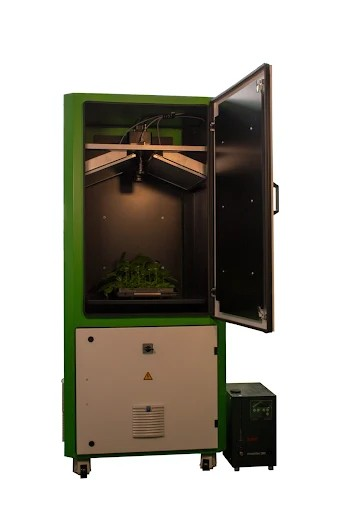
\includegraphics[width=\textwidth]{Images/Lemnatec}
        \caption{LemnaTec High-Throughput Greenhouse System.}
        \label{fig:lemnatec}
    \end{subfigure}
    \hfill
    \begin{subfigure}[b]{0.3\textwidth}
        \centering
        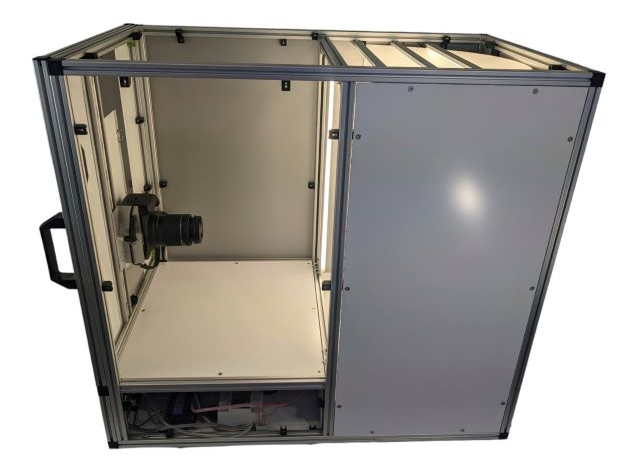
\includegraphics[width=\textwidth]{Images/phenobox}
        \caption{PhenoBox Research Enclosure.}
        \label{fig:phenobox}
    \end{subfigure}
    \hfill
    \begin{subfigure}[b]{0.3\textwidth}
        \centering
        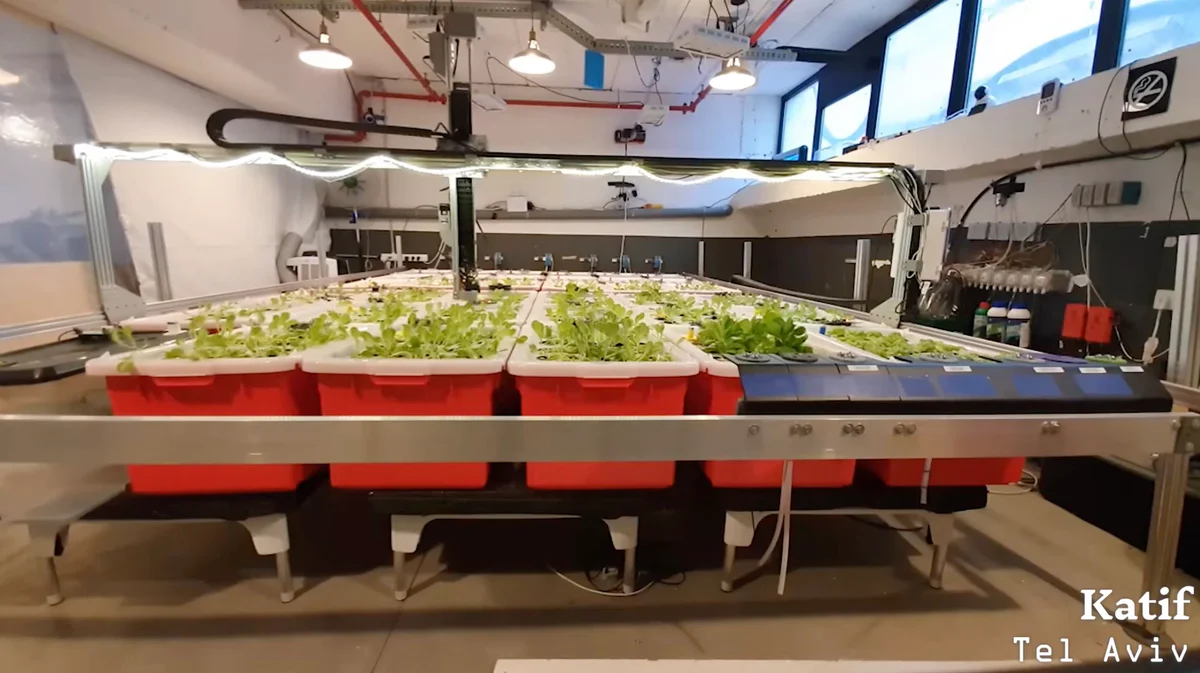
\includegraphics[width=\textwidth]{Images/farmbot}
        \caption{FarmBot Open-Source Precision Agriculture Robot.}
        \label{fig:farmbot}
    \end{subfigure}
    \caption[Commercial, Open-Source and Educational Phenotyping Reference Systems]{Representative phenotyping platforms across market/price tiers. LemnaTec \parencite{lemnatec-solutions, vienna-scientific-phenobox} and PhenoBox are commercial high-throughput systems that are designed for research institutions. These emphasize throughput and total environmental control. FarmBot \parencite{farmbot} is a community-maintained open-source robot that illustrates the modular and affordable end of the spectrum. All three contrast with the portable, educational focus of PhenoHive .}
    \label{fig:reference-collage}
\end{figure}

\section{Educational platforms for plant biology}

In academic settings, plant physiology and botany courses often depend on manual measurements, shared greenhouse facilities, or pre-recorded datasets. Several institutions have developed open-source platforms for continuous plant monitoring in teaching and research contexts. Phenotiki \parencite{minervini2017phenotiki} is an example of a Raspberry Pi-based platform for image-based phenotyping of rosette plants, designed to lower the barrier to entry for laboratory use. The Growth Monitor Pi (GMPi) \parencite{grindstaff2019gmpi} similarly targets affordable remote monitoring of plant growth in facilities, using single-board computers to enable continuous observation without dedicated infrastructure. The diversity of these approaches reflects different pedagogical goals. Some platforms emphasize instrumentation, while others prioritize biological observation and interpretation. The PhenoHive project follows the second approach, where technology is a tool for observation rather than the primary subject of study.

Autonomous monitoring addresses a timescale mismatch. The physiological processes students are asked to observe acclimation responses, growth allocation, VPD-driven stomatal behavior unfold over days and weeks, not laboratory hours. Continuous sensors also remove the greenhouse bottleneck, letting twenty groups run parallel experiments with different conditions simultaneously. The reduction in collection overhead shifts student attention from measurement logistics toward experimental design and biological interpretation.
The biological signals that make this extended monitoring valuable are grouped into four measurement domains (Table~\ref{tab:phenotyping-metrics-interpretation}).
\begin{table}[H]
\centering
\caption[Core Phenotyping Metrics and Physiological Interpretation]{Core metrics used in plant phenotyping and their physiological interpretation. Environmental, light, mass and morphology signals are not interpreted independently; they are jointly used to reason about transpiration, photosynthesis and growth dynamics over time.}
\label{tab:phenotyping-metrics-interpretation}
\footnotesize
\setlength{\tabcolsep}{5pt}
\renewcommand{\arraystretch}{1.2}
\begin{tabularx}{\textwidth}{|P{2.5cm}|X|X|}
\hline
\textbf{Measurement domain} & \textbf{Primary metrics} & \textbf{Physiological interpretation} \\
\hline
Environment & Air temperature, relative humidity, vapor pressure deficit (VPD) & Transpiration behavior, stomatal context, stress exposure \\
\hline
Light & Intensity and spectral composition & Photosynthetic context, acclimation response \\
\hline
Mass & Pot mass trend and short-term variation & Water-balance dynamics, biomass accumulation trajectory \\
\hline
Imaging & Projected leaf area, canopy color, shape descriptors & Growth progression, visual stress signatures \\
\hline
\end{tabularx}

\vspace{0.4em}
{\footnotesize Cross-cutting quality dimensions: temporal continuity, sampling interval and data quality (missing values, outliers, drift).}
\end{table}
PhenoHive is specifically designed for this teaching context, where the primary goal is pedagogical understanding and where stations may be deployed in diverse, uncontrolled environments such as student homes. Table~\ref{tab:platform-landscape-comparison} positions PhenoHive within this field.
\begin{table}[H]
\centering
\caption[Phenotyping Platform Families Comparison]{Comparison of plant phenotyping platform families across cost, throughput, modalities, deployment context and teaching access. Commercial systems maximize automation, while open-source and educational platforms prioritize flexibility and affordability.}
\label{tab:platform-landscape-comparison}

\footnotesize
\setlength{\tabcolsep}{4pt}
\renewcommand{\arraystretch}{1.25}
\rowcolors{2}{gray!8}{white}
\begin{tabularx}{\textwidth}{P{2.6cm}Y Y Y Y}
\textbf{Criterion} & \textbf{Commercial} & \textbf{Open-source} & \textbf{Educational} & \textbf{PhenoHive (this thesis)} \\
\hline
Cost & High & Moderate & Low & Low ($\sim$€137/unit) \\
Throughput & Very high & Medium & Low & Low (1 plant/station) \\
Main modalities & RGB, multispectral, thermal, mass, climate, often gas exchange & RGB, multispectral, thermal, mass, optional custom sensors & RGB, mass, basic climate, optional light/humidity add-ons & Temp./humidity, 14-channel spectral (calibrated), mass, RGB camera \\
Deployment context & Controlled greenhouse/chamber, dedicated server, high maintenance & Lab/greenhouse, local server or SBC, moderate integration effort & Desk or small enclosure, minimal infrastructure & Student home or desk; single USB supply; Tailscale overlay \\
Typical users & Industry breeding and research centers & Research labs and student projects & Course cohorts and teaching labs & LBIR1251 student groups ($\sim$20 parallel stations) \\
Teaching accessibility & \textit{Low} & \textit{Moderate} & \textbf{High} & \textbf{High} \\
\end{tabularx}
\rowcolors{2}{}{}

\vspace{0.5em}
{\footnotesize Synthesis based on literature and prior PhenoHive theses \parencite{goffinet2024, colinet2025}. PhenoHive sits in the educational cost tier but targets open-source-tier sensing quality through laboratory-validated sensors.}
\end{table}

\section{Sensor integration and measurement strategy}

Sensor selection and integration demonstrate a recurring trade-off between price and precision. High-end phenotyping platforms often integrate many sensors and cameras, which provides multispectral, thermal and morphological data at the same time. This completeness comes with higher complexity, cost and data volume. Educational platforms usually favor a more focused approach, selecting a smaller set of sensors that directly serve learning objectives.

Four variables have the most direct pedagogical value for plant physiology. Spectral light quality and illuminance drive photosynthesis and control developmental responses through phytochrome \parencite{franklin2005phytochromes}. Air temperature and relative humidity jointly determine vapor pressure deficit, which governs stomatal conductance and evapotranspiration \parencite{allen1998fao}. Continuous pot mass provides a slow, integrating water-balance signal; combined with camera images it traces biomass accumulation along two independent lines of evidence.

In many existing platforms, sensor choices reflect availability and budget constraints more than strict pedagogical optimization. In the PhenoHive project's sequence, \textcite{goffinet2024} and \textcite{colinet2025} established a baseline that made continuous environmental and growth observation feasible in an educational context. Their work also showed which variables needed stronger characterization in later iterations.

The VPD and the spectral band ratio carry the most direct pedagogical relevance of the four. Both need precisely calibrated sensors which is what drives the sensor selection in Chapter~\ref{ch:data-acquisition}. Not only that but with 20 groups running in parallel, the measurements also have to stay consistent and comparable. If they aren't, this means that no group can trust the conclusions it draws from its own experiment.

\section{Synthesis of previous PhenoHive theses}

The two previous PhenoHive theses advanced the platform in concrete, distinct steps (Figure~\ref{fig:phenohive-timeline}). \textcite{goffinet2024} established the continuous-monitoring feasibility on DietPi, modularised the codebase and provided the first automated deployment pipeline with a self-hosted visualization stack. \textcite{colinet2025} upgraded the hardware, improved the image-analysis pipeline with shadow detection, migrated the visualization infrastructure to an online server, and added first-generation environmental sensors (a resistive soil moisture probe and a photoresistor). Considered together, these works demonstrate a clear progression in platform maturity. What they also reveal is the gap between having a sensor \emph{connected} and having a signal that is \emph{metrologically grounded} and \emph{physiologically informative}. The soil moisture index cannot substitute for air humidity in VPD calculations, and a photoresistor cannot discriminate the spectral bands that drive phytochrome-mediated plant responses.

This review of the state of the art in plant phenotyping platforms, and of the PhenoHive project's trajectory, all show that for a platform to be effective, it must be reliable, accurate and pedagogically relevant. Also, keeping the platform easily maintainable and extensible is critical for its long-term success in an educational setting. The next chapters will therefore cover detail how the current iteration of PhenoHive addresses these requirements through sensor calibration, software architecture refactor and deployment strategy improvements.


\begin{figure}[H]
\centering
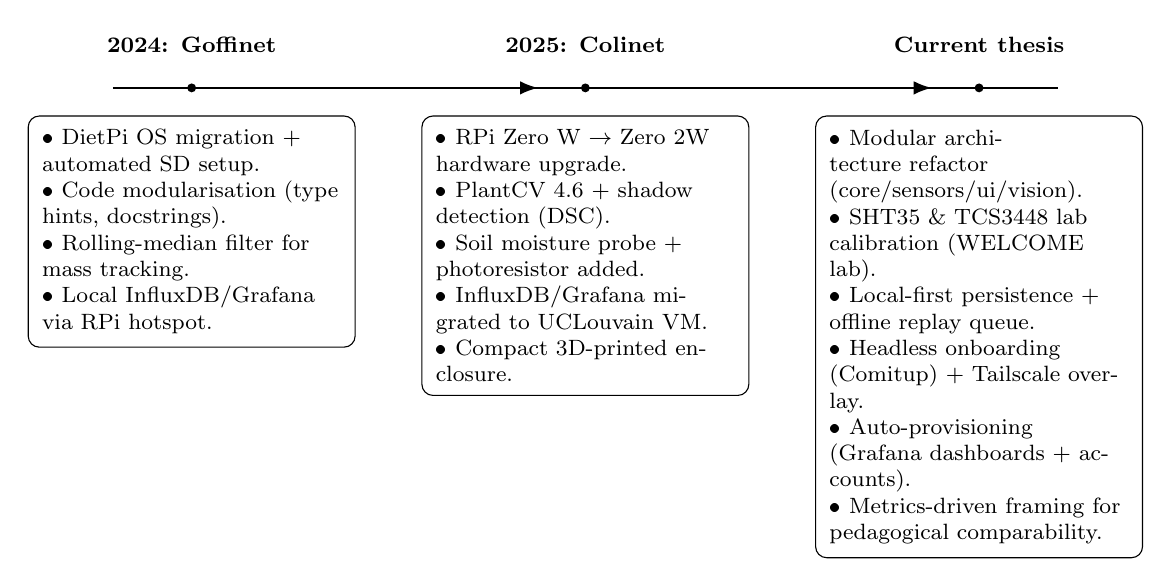
\begin{tikzpicture}[
    milestone/.style={draw, rounded corners, align=left, text width=3.8cm, inner sep=5pt, font=\footnotesize},
    title/.style={font=\bfseries\footnotesize, align=center},
    flowarrow/.style={-{Latex[length=2.3mm]}, thick}
]
% Timeline axis
\draw[thick] (0,0) -- (12,0);

% Milestone markers
\fill (1,0) circle (1.6pt);
\fill (6,0) circle (1.6pt);
\fill (11,0) circle (1.6pt);

% Direction arrows
\draw[flowarrow] (1.6,0) -- (5.4,0);
\draw[flowarrow] (6.6,0) -- (10.4,0);

% Titles above markers
\node[title] at (1,0.55) {2024: Goffinet};
\node[title] at (6,0.55) {2025: Colinet};
\node[title] at (11,0.55) {Current thesis};

% Description boxes below the timeline
\node[milestone, anchor=north] at (1,-0.35) {
\textbullet\ DietPi OS migration + automated SD setup.\\
\textbullet\ Code modularisation (type hints, docstrings).\\
\textbullet\ Rolling-median filter for mass tracking.\\
\textbullet\ Local InfluxDB/Grafana via RPi hotspot.
};

\node[milestone, anchor=north] at (6,-0.35) {
\textbullet\ RPi Zero W $\rightarrow$ Zero 2W hardware upgrade.\\
\textbullet\ PlantCV 4.6 + shadow detection (DSC).\\
\textbullet\ Soil moisture probe + photoresistor added.\\
\textbullet\ InfluxDB/Grafana migrated to UCLouvain VM.\\
\textbullet\ Compact 3D-printed enclosure.
};

\node[milestone, anchor=north] at (11,-0.35) {
\textbullet\ Modular architecture refactor (core/sensors/ui/vision).\\
\textbullet\ SHT35 \& TCS3448 lab calibration (WELCOME lab).\\
\textbullet\ Local-first persistence + offline replay queue.\\
\textbullet\ Headless onboarding (Comitup) + Tailscale overlay.\\
\textbullet\ Auto-provisioning (Grafana dashboards + accounts).\\
\textbullet\ Metrics-driven framing for pedagogical comparability.
};
\end{tikzpicture}

\vspace{0.4em}
{\footnotesize \textbf{Overall trajectory:} feasibility \& automation $\rightarrow$ hardware upgrade \& image quality \& VM migration $\rightarrow$ modular architecture \& metrological calibration \& operational hardening.}

\vspace{0.2em}
{\footnotesize Scope note: timeline summarizes thesis-level contributions, not full implementation details.}
\caption[Evolution of the PhenoHive Platform]{Evolution of the PhenoHive platform across consecutive theses where each one contributes a distinct step to the maturation of the platform as a whole. From initial feasibility to expanded observation and metrics-driven pedagogical framing.}
\label{fig:phenohive-timeline}
\end{figure}

\chapter{Requirements and approach}
\label{ch:requirements}

Turning a proof-of-concept into a platform that can actually be deployed means that the first step is to pin down what it has to do. Chapter~\ref{ch:introduction} framed the work around three objectives: architectural clarity~(O1), sensing quality~(O2), and operational reliability~(O3). This chapter translates those into six concrete, verifiable requirements. R1 operationalizes sensing quality (O2); R5 captures the architectural maintainability goal (O1); R3, R4, and R6 together address operational reliability (O3). R2 is a system constraint set by the deployment context — 20 simultaneous stations on a teaching budget — rather than derived from any single objective, and it applies across all three.

\section{Pedagogical requirements}

\textbf{Requirement 1:} The system should provide calibrated sensor data within uncertainty bounds small enough to support physiologically meaningful analysis. More specifically, VPD calculations that are traceable to reference instruments and spectral discrimination at the red/far-red band boundary.

\textbf{Design approach:} This asks the sensors to be able to resolve two things. One is the VPD gradient that drives stomatal response and the other is the red/far-red boundary that triggers phytochrome-mediated responses. Both of these require much more precision than what basic temperature/humidity or RGB sensors can provide (Figure~\ref{fig:vpd-calculation}). Chapter~\ref{ch:data-acquisition} works through the calibration method and the resulting uncertainty budgets.

\begin{figure}[H]
    \centering
    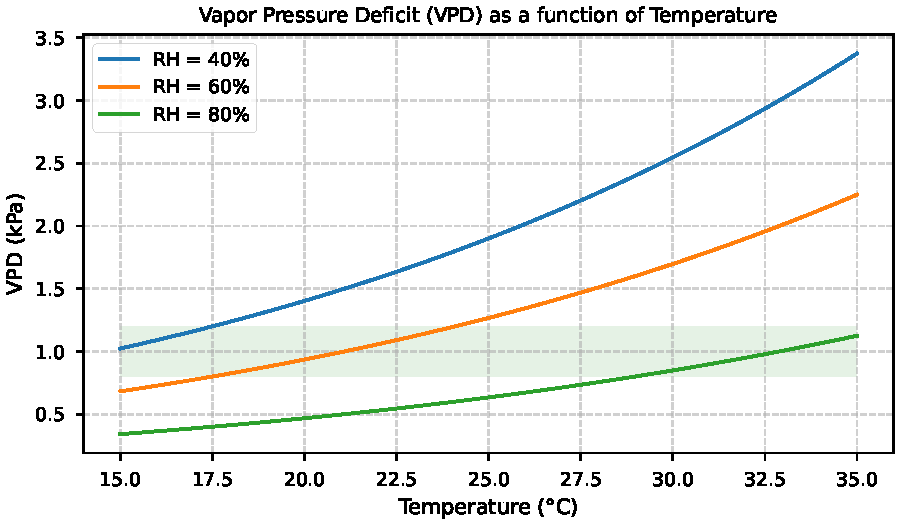
\includegraphics[width=0.85\textwidth]{Images/vpd_calculation}
    \caption[Temperature, Humidity, and Vapor Pressure Deficit]{The relationship between temperature, relative humidity, and the Vapor Pressure Deficit (VPD). Precise biological modeling of transpiration requires high-precision sensors because subtle errors in humidity translate to significant errors in VPD calculation, increasing at higher temperatures.}
    \label{fig:vpd-calculation}
\end{figure}

\section{Hardware and budget constraints}

\textbf{Requirement 2:} The total hardware cost per station should not exceed €150 as this enables simultaneous deployment of approximately 20 units within a teaching budget.

\textbf{Design approach:} The budget cap motivates each choice of component. Twenty groups each need a station at the same time, so each part has to earn its place on precision against cost. Commercial platforms can rely on more expensive industrial controllers where PhenoHive instead pairs a Raspberry Pi single-board computer with low-cost, I$^2$C-compatible sensors. I kept the Raspberry Pi over a cheaper microcontroller like an ESP32 because of the headroom. It can run a full Linux system, drive the high-resolution camera used for morphological tracking and manage a local persistence stack without needing to rely on a constant cloud connection.

Appendix~\ref{ch:appendix-bom} contains the full bill of materials. A unit comes to about €137 (Table~\ref{tab:bom}).


\section{Deployment context and operational resilience}

The stations are meant mainly for students' homes, but they should also work in a traditional greenhouse if need be. A home setting brings its own problems: power can get unplugged by accident, home Wi-Fi may be unstable or get reconfigured, and the surrounding environment is neither controlled nor steady.

\textbf{Requirement 3 (R3):} The system should not lose data during network outages and should recover connectivity autonomously, resuming data transmission without user intervention.

\textbf{Design approach:} The solution is an offline-first persistence model: measurements are written locally first and pushed to InfluxDB whenever it is reachable. When a push fails, the record is added to a local JSONL queue that replays on reconnection (Figure~\ref{fig:resilience-model}). Chapters~\ref{ch:storage} and~\ref{ch:evaluation} cover the design and the 48-hour disconnection test.

\textbf{Requirement 4 (R4):} First-boot setup should complete in under five minutes with no command-line interaction, so that students can begin collecting data immediately after connecting the device to Wi-Fi.

\textbf{Design approach:} On first boot, the \texttt{comitup} service broadcasts a temporary Wi-Fi hotspot. The student connects to it and enters the home network credentials through a captive portal in a web browser. The station then joins the network and starts pushing data automatically. Chapter~\ref{ch:evaluation} measures the end-to-end timing for each phase.

\begin{figure}[H]
\centering
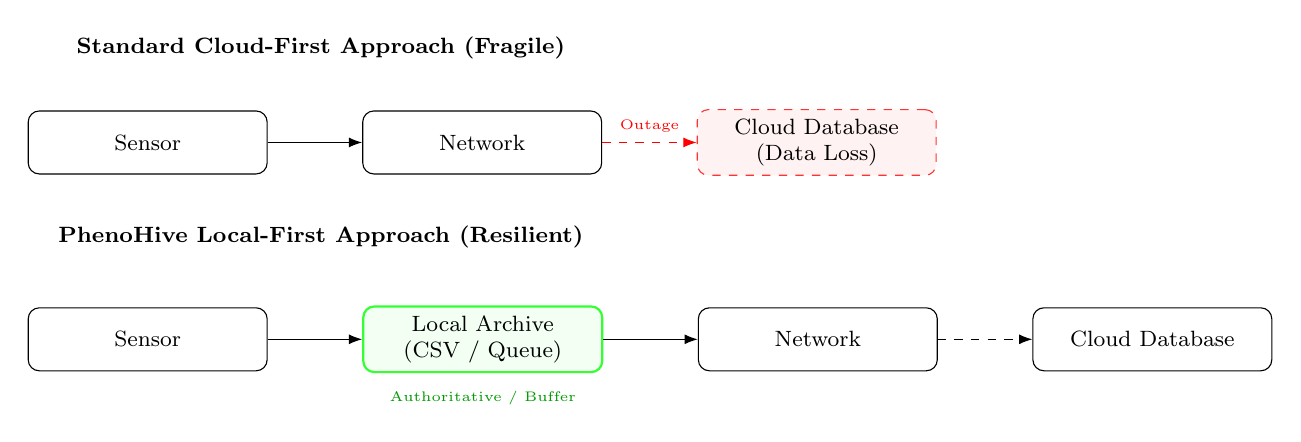
\begin{tikzpicture}[
    node distance=0.8cm and 1.2cm,
    box/.style={draw, rounded corners, align=center, text width=2.8cm, minimum height=0.8cm, font=\footnotesize},
    fail/.style={draw=red!80, fill=red!5, dashed},
    success/.style={draw=green!80, fill=green!5, thick}
]
% Cloud-First
\node[font=\bfseries\footnotesize] (label1) at (2.2,1.2) {Standard Cloud-First Approach (Fragile)};
\node[box] (s1) at (0,0) {Sensor};
\node[box, right=of s1] (n1) {Network};
\node[box, right=of n1, fail] (db1) {Cloud Database\\(Data Loss)};
\draw[-{Latex}] (s1) -- (n1);
\draw[-{Latex}, red, dashed] (n1) -- (db1) node[midway, above, font=\tiny] {Outage};

% Local-First
\node[font=\bfseries\footnotesize] (label2) at (2.2,-1.2) {PhenoHive Local-First Approach (Resilient)};
\node[box] (s2) at (0,-2.5) {Sensor};
\node[box, right=of s2, success] (l2) {Local Archive\\(CSV / Queue)};
\node[box, right=of l2] (n2) {Network};
\node[box, right=of n2] (db2) {Cloud Database};

\draw[-{Latex}] (s2) -- (l2);
\draw[-{Latex}] (l2) -- (n2);
\draw[-{Latex}, dashed] (n2) -- (db2);
\node[below=0.1cm of l2, font=\tiny, text=green!60!black] {Authoritative / Buffer};
\end{tikzpicture}
\caption[Comparison of Data Persistence Strategies]{Two data-persistence strategies side by side. A standard cloud-first design is fragile because when the link to the cloud database drops during an outage, the readings in transit are lost. PhenoHive first writes to a local archive (CSV and queue) and treats it as authoritative, so an outage interrupts the upload and not the record.}
\label{fig:resilience-model}
\end{figure}

\section{Maintainability and handoff}

Teaching tools at a university change hands constantly so having a tightly coupled, monolithic codebase is a liability because a new TA who wants to add a sensor or change a setting has to touch the acquisition loop and can break it without realising.

\textbf{Requirement 5 (R5):} A new TA with no knowledge of the codebase should be able to add a new sensor and to modify a configuration value without having to modify the main core acquisition loop.

\textbf{Design approach:} The architecture has to be as modular and configuration-driven as possible. All of the sensor drivers, the core acquisition loop and the persistence therefore need to live each as distinct and testable components that can be changed, swapped out and tested one at a time.

\section{Data isolation and access control}

With 20 groups all writing to one central database at once, there is a real risk of data bleeding across groups. Each student should only be able to see and analyse their own station's data, so that their experimental hypotheses stay their own.

\textbf{Requirement 6 (R6):} Each student group should only have access to data from their own station. This should be enforced both on the Grafana permission layer and the InfluxDB query layer in order to maintain data integrity and isolation.

\textbf{Design approach:} A \texttt{station\_id} tag is added to the data at acquisition and stays with it throughout the whole pipeline. Grafana folder permissions and Flux queries filter each block cross-group access on their own. this makes it so that neither layer is a single point of failure. Chapter~\ref{ch:storage} covers the implementation.

\section{Requirements summary}

\begin{table}[htbp]
\centering
\caption[System-Level Requirements Summary]{Consolidated system-level requirements with traceability to the three objectives from Chapter~\ref{ch:introduction}: 1~architectural clarity, 2~sensing quality, 3~operational reliability. The verification column references the test or evidence that demonstrates compliance in Chapter~\ref{ch:evaluation}.}
\label{tab:requirements-summary}
\small
\setlength{\tabcolsep}{5pt}
\renewcommand{\arraystretch}{1.2}
\begin{tabularx}{\textwidth}{|P{0.8cm}|X|P{2.8cm}|P{1.1cm}|}
\hline
\textbf{ID} & \textbf{Requirement} & \textbf{Verification} & \textbf{Obj.} \\
\hline
R1 & Calibrated sensor data within research-grade uncertainty for VPD and spectral analysis & §\,\ref{sec:sht35-calibration}, §\,\ref{sec:tcs3448-calibration} & 2 \\
\hline
R2 & Total hardware cost $\leq$\,€150 per station & Appendix~\ref{ch:appendix-bom} & 1--3 \\
\hline
R3 & No data loss during network outages of $\geq$\,48\,h; full replay upon reconnection & 48\,h disconnection test (§\,\ref{ch:evaluation}) & 3 \\
\hline
R4 & First-boot setup in $<$\,5\,minutes with no command-line interaction & First-boot test (§\,\ref{ch:evaluation}) & 3 \\
\hline
R5 & New sensor addable without modifying the acquisition loop; configuration-driven extension & §\,\ref{ch:architecture} & 1 \\
\hline
R6 & Per-group data isolation enforced at both Grafana permission and InfluxDB query levels & Multi-station isolation test (§\,\ref{ch:evaluation}) & 3 \\
\hline
\end{tabularx}
\end{table}


\chapter{System architecture}
\label{ch:architecture}

This iteration's architecture is compact, and each part has a clear job, but it did not get there in one step. I reached the current structure by decoupling responsibilities that had started out too tightly coupled, since the monolithic approach made later changes hard to implement. The system now rests on a small set of components, each with a specific role in the measurement chain: configuration, sensor instantiation, acquisition, persistence, time alignment, and local user feedback. For a teaching platform that division is critical, because the design stays readable and maintainable, and it holds up when one part of the stack fails.

The runtime reads a simple config file, builds the sensor objects, starts the time-sync and debug services and enters the measurement loop (Figure~\ref{fig:system-architecture-runtime-flow}). Each measurement cycle creates a single flattened record which holds data from every active sensor. That record is written locally first and only then forwarded to the remote time-series backend if it is reachable. The order matters because when the network drops, the dashboard can go stale while acquisition keeps on working.

If this local-first writing approach is not implemented, this would mean that every short connectivity drop would leave a visible gap in the data's timeline because the records made during the outage would be lost. This approach also means that the queued records are replayed once the link to the server is restored. A 48-hour disconnection test in Chapter~\ref{ch:evaluation} confirms this requirement on physical hardware.

\begin{figure}[H]
\centering
\resizebox{\textwidth}{!}{%
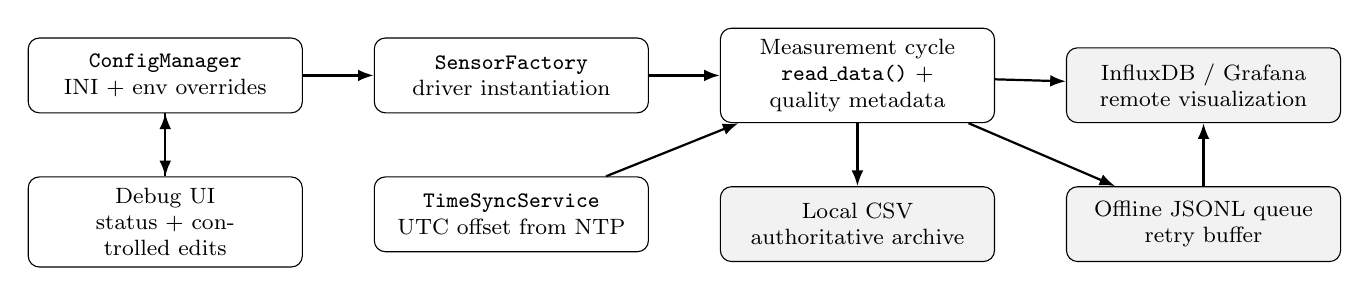
\begin{tikzpicture}[
    node distance=0.8cm and 0.9cm,
    block/.style={draw, rounded corners, align=center, text width=3.2cm, minimum height=0.95cm, inner sep=4pt, font=\footnotesize},
    store/.style={draw, rounded corners, align=center, text width=3.2cm, minimum height=0.95cm, inner sep=4pt, font=\footnotesize, fill=gray!10},
    arrow/.style={-{Latex[length=2mm]}, thick},
]
\node[block] (cfg) {\texttt{ConfigManager}\\INI + env overrides};
\node[block, right=of cfg] (factory) {\texttt{SensorFactory}\\driver instantiation};
\node[block, right=of factory] (loop) {Measurement cycle\\\texttt{read\_data()} + quality metadata};

\node[store, below=of loop] (csv) {Local CSV\\authoritative archive};
\node[store, right=of csv] (queue) {Offline JSONL queue\\retry buffer};
\node[store, above=of queue] (influx) {InfluxDB / Grafana\\remote visualization};
\node[block, below=of cfg] (debug) {Debug UI\\status + controlled edits};
\node[block, below=of factory] (sync) {\texttt{TimeSyncService}\\UTC offset from NTP};

\draw[arrow] (cfg) -- (factory);
\draw[arrow] (factory) -- (loop);
\draw[arrow] (loop) -- (csv);
\draw[arrow] (loop) -- (influx);
\draw[arrow] (loop) -- (queue);
\draw[arrow] (queue) -- (influx);
\draw[arrow] (sync) -- (loop);
\draw[arrow] (cfg) -- (debug);
\draw[arrow] (debug) -- (cfg);
\end{tikzpicture}
}
\caption[System Architecture Runtime Data Flow]{Runtime data flow from configuration and sensor acquisition to local persistence, remote synchronization and user feedback.}
\label{fig:system-architecture-runtime-flow}
\end{figure}

\section{Codebase structure and module boundaries}

The runtime entry point is in \texttt{main.py} and the implementation responsibilities are grouped under \texttt{src/}. The \texttt{src/core/} package contains orchestration and shared services (configuration management, sensor factory logic, persistence, logging and time synchronization). Hardware-specific drivers are isolated in \texttt{src/sensors/}, so sensor changes do not require edits in the runtime loop. The debug dashboard is separated in \texttt{src/ui/}, where the dashboard and HTTP service are implemented. Image-processing logic is grouped in \texttt{src/vision/} so camera-related code stays independent from numeric sensor acquisition. The structure is completed by \texttt{tests/}, which validates core behavior and sensor integration points and \texttt{scripts/}, which contains deployment and maintenance scripts. For TAs, this folder layout easily shows where to look when an update is needed (Figure~\ref{fig:module-boundaries} and Table~\ref{tab:system-architecture-project-structure}).

\begin{figure}[H]
\centering
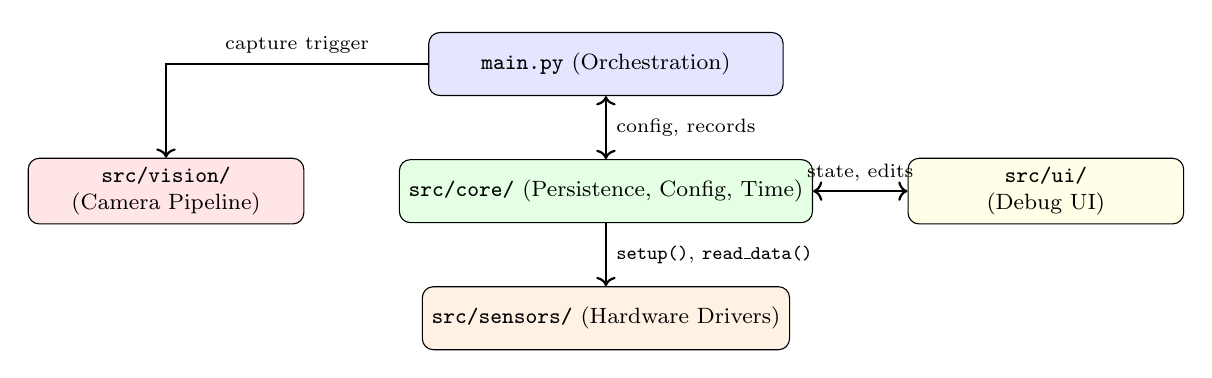
\begin{tikzpicture}[
    node distance=0.8cm and 1.2cm,
    layer/.style={draw, rectangle, rounded corners, minimum width=4.5cm, minimum height=0.8cm, align=center, fill=gray!5, font=\footnotesize}
]
\node[layer, fill=blue!10] (main) {\texttt{main.py} (Orchestration)};
\node[layer, below=of main, fill=green!10] (core) {\texttt{src/core/} (Persistence, Config, Time)};
\node[layer, below=of core, fill=orange!10] (sensors) {\texttt{src/sensors/} (Hardware Drivers)};
\node[layer, left=of core, minimum width=3.5cm, fill=red!10] (vision) {\texttt{src/vision/}\\(Camera Pipeline)};
\node[layer, right=of core, minimum width=3.5cm, fill=yellow!10] (ui) {\texttt{src/ui/}\\(Debug UI)};

\draw[<->, thick] (main) -- (core) node[midway, right, font=\scriptsize] {config, records};
\draw[->, thick] (core) -- (sensors) node[midway, right, font=\scriptsize] {\texttt{setup()}, \texttt{read\_data()}};
\draw[->, thick] (main.west) -| (vision.north) node[near start, above, font=\scriptsize] {capture trigger};
\draw[<->, thick] (core) -- (ui) node[midway, above, font=\scriptsize] {state, edits};
\end{tikzpicture}
\caption[PhenoHive Module Boundaries]{Module boundaries and architectural layers of the PhenoHive codebase.}
\label{fig:module-boundaries}
\end{figure}

\begin{table}[H]
\centering
\caption[PhenoHive Project Structure]{Project structure used to enforce architectural boundaries and maintenance ownership.}
\label{tab:system-architecture-project-structure}
\small
\setlength{\tabcolsep}{5pt}
\renewcommand{\arraystretch}{1.2}
\begin{tabularx}{\textwidth}{|P{2.9cm}|P{3.8cm}|X|}
\hline
\textbf{Layer} & \textbf{Project files} & \textbf{Primary responsibility} \\
\hline
Runtime entry point & \texttt{main.py} & Application bootstrap, service startup and main acquisition loop. \\
\hline
Core services & \texttt{src/core/} & Configuration loading, sensor factory, persistence logic, time synchronization and shared runtime policies. \\
\hline
Sensor drivers & \texttt{src/sensors/} & Hardware-specific sensor setup and acquisition APIs. \\
\hline
Debug interface & \texttt{src/ui/} & Debug dashboard, local status inspection and controlled runtime configuration updates. \\
\hline
Vision pipeline & \texttt{src/vision/} & Camera capture and image-based phenotyping path separated from numeric sensing. \\
\hline
Validation and operations & \texttt{tests/}, \texttt{scripts/} & Automated checks and maintenance helpers used by TAs. \\
\hline
\end{tabularx}
\end{table}

\section{Configuration and runtime composition}

The configuration layer is intentionally more defensive than just a raw INI parser. The \texttt{ConfigManager} wraps \texttt{configparser} with typed getters, environment-variable overrides and a uniform fallback strategy. This means that the same configuration source can be used both for normal operation and for deployment on student machines where some values can be injected by the environment.

This means that the runtime stays flexible without turning configuration into a second program. The bootstrap stays simple. It only reads one configuration file, resolves the overrides and then hands a small set of typed values to the rest of the system.

\section{Sensor abstraction and hardware binding}

Sensor construction is handled by a factory instead of through an inline in the main loop. The \texttt{SensorFactory} is what holds the mapping from the configuration values to the concrete sensor classes in one place. It's because of this that the  mapping is centralised, the runtime has no hardware-specific branching and extending the sensor set stays a controlled and local change that doesn't affect the rest of the system.

The factory currently builds the air temperature and humidity sensor, the light sensor, and the HX711-based scale. Each exposes the same lifecycle: \texttt{setup()} to check that it is usable and \texttt{read\_data()} to return one measurement payload. This shared contract matters more than the specific hardware because it lets the rest of the system treat every sensor as an interchangeable producer of timestamped data.

I intentionally did not reimplement the plant-camera pipeline. It's reused from the previous thesis following the discussions on the requirements choices made before implementation. This fits the methodology I followed throughout the project which is to keep the stable components that already do their job well.

\section{Measurement cycle and orchestration}

The main runtime is centered on a measurement cycle that collects data from all sensors, normalizes it and produces one record for storage. This cycle supports burst sampling and aggregation to reduce short-term variability before interpretation. It also tracks plausibility ranges, success ratios and quality indicators such as coefficient of variation. This means that it keeps uncertainty and outlier sensitivity explicit instead of hiding them in a single final value. I adopted burst sampling over single-read cycles because single reads can produce unstable values that degrade overall data quality. Figure~\ref{fig:two-tier-timing} illustrates the decoupling between the fast collection interval and the slower publish interval.

Instead of setting the OS clock, the runtime applies a UTC offset in application space through \texttt{TimeSyncService}. This makes it a lot simpler to run. If the NTP synchronization fails, the system falls back to the local clock and logs the failure in the diagnostics.

\begin{figure}[H]
\centering
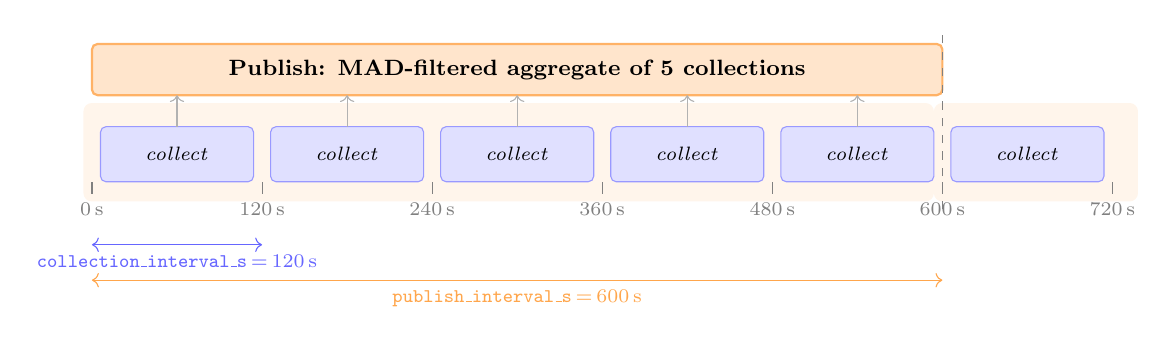
\begin{tikzpicture}[x=1.08cm, y=1cm, font=\scriptsize]
% Background shading for first publish window
\fill[orange!8, rounded corners=3pt] (-0.1,-0.2) rectangle (9.9, 1.05);
% Second window (partial)
\fill[orange!8, rounded corners=3pt] (9.9,-0.2) rectangle (12.3, 1.05);

% Collection blocks (5 per window, at 0, 2, 4, 6, 8 units)
\foreach \i in {0,2,4,6,8} {
    \draw[fill=blue!12, draw=blue!40, rounded corners=2pt]
        (\i+0.1, 0.05) rectangle (\i+1.9, 0.75);
    \node at (\i+1.0, 0.40) {\textit{collect}};
}
% First block of next window
\draw[fill=blue!12, draw=blue!40, rounded corners=2pt]
    (10.1, 0.05) rectangle (11.9, 0.75);
\node at (11.0, 0.40) {\textit{collect}};

% Timestamps on x-axis
\foreach \x/\t in {0/{0\,s}, 2/{120\,s}, 4/{240\,s}, 6/{360\,s}, 8/{480\,s}, 10/{600\,s}, 12/{720\,s}} {
    \draw[thin, gray] (\x,-0.1) -- (\x, 0.05);
    \node[below, text=gray] at (\x,-0.1) {\t};
}

% Publish bar
\draw[fill=orange!20, draw=orange!60, rounded corners=2pt, thick]
    (0, 1.15) rectangle (10, 1.8);
\node[font=\footnotesize\bfseries] at (5, 1.475)
    {Publish: MAD-filtered aggregate of 5 collections};

% Arrows from each collection to publish bar
\foreach \i in {0,2,4,6,8} {
    \draw[->, thin, gray!60] (\i+1.0, 0.75) -- (\i+1.0, 1.15);
}

% Dashed separator at window boundary
\draw[dashed, gray, thin] (10,-0.3) -- (10, 2.0);

% Dimension arrows
\draw[<->, blue!60, thin] (0,-0.75) -- (2,-0.75)
    node[midway, below, font=\scriptsize]
    {\texttt{collection\_interval\_s}\,=\,120\,s};
\draw[<->, orange!70, thin] (0,-1.2) -- (10,-1.2)
    node[midway, below, font=\scriptsize]
    {\texttt{publish\_interval\_s}\,=\,600\,s};
\end{tikzpicture}
\caption[Two-Tier Measurement Timing]{Two-tier timing of the measurement loop. Raw sensor bursts (\textit{collect}) fire at the fast \texttt{collection\_interval\_s} (default 120\,s). Once the \texttt{publish\_interval\_s} window (default 600\,s) closes, the five collected records are filtered and aggregated into one smoothed record that is persisted and forwarded. Filtering then occurs on two levels. First, a MAD outlier pass within each individual burst's raw reads. Second, another filter pass across the collection records at publish time (see Section~\ref{sec:data-smoothing}). This decoupling keeps noisy individual reads from corrupting data reads without sacrificing the overall multi-sample noise rejection within each window. }
\label{fig:two-tier-timing}
\end{figure}

\section{Persistence and remote synchronization}

Persistence is split into a local authoritative layer and a remote synchronization layer. The \texttt{DataManager} always appends the record to the local file first. That file is the main archive and it remains usable even if no remote service is reachable. After the local write, the same record is pushed to InfluxDB when it's able to do so. If that push fails, then the record is added to a JSONL offline queue and retried later.

A network error should not create data loss and a temporary backend failure should not interrupt the station. Keeping local CSV as the first storage step and treating InfluxDB as a synchronization target allows immediate visualization and offline recovery without having to introduce a heavier broker or database layer.

What reaches InfluxDB is purposefully filtered. Only stable numeric fields become measurements and any high-cardinality or free-form strings will stay behind in the CSV archive. This allows the remote schema to stay simple and fast, while at the same time the local archive still holds everything just in case for later analysis or debugging.

\section{Debug interface and local feedback}

The local debug UI exposes the current status, configuration views and limited config-editing capabilities through a lightweight Hypertext Transfer Protocol (HTTP) server. It is not intended to replace a full administration interface. It is a focused tool meant for inspection, diagnosis and controlled parameter changes during deployment by both students and TAs.

The interface has several guards built in. Students cannot change the settings or view safety critical information while TAs can by entering a password. Some options cannot be edited at all because they are safety-critical or tied to the hardware. So the debug UI works more as a local maintenance platform used to supervise the correct functioning of the station instead of it being a general-purpose control plane.

This choice is completely intentional. The platform does not bury its operational complexity under a large management stack. It instead keeps the maintenance path visible and constrained which allows it to answer the requirement of keeping the system easily maintainable and robust for potential future changes.


\chapter{Data acquisition and processing}
\label{ch:data-acquisition}

This chapter covers the sensor suite, the laboratory calibration that traces each channel to a known physical reference and the two-stage noise-rejection pipeline that filters raw readings before they reach storage.

\section{Sensor suite}

The platform combines three numeric measurement domains with one visual observation path:
\begin{itemize}
    \item \textbf{Air conditions}: The SHT35 sensor measures air temperature and relative humidity via the I$^2$C bus \parencite{seeed-sht35}. Its $\pm$1.5\% relative humidity (RH) and $\pm$0.1$^\circ$C accuracy \parencite{sensirion-sht35} is the technical foundation for the system's VPD calculations \parencite{massmann2019vpd}. 
    \item \textbf{Light spectrum}: The TCS3448 (Color 21 Click \parencite{mikroe-color-21}) reads light on 14 separate channels. It has eight narrow-band filters (F1--F8), three broad "Commission Internationale de l'Éclairage" (CIE) XYZ-type channels (FZ$\,\leftrightarrow\,$Z tristimulus, FY$\,\leftrightarrow\,$Y/luminance, FXL$\,\leftrightarrow\,$X-long wavelength), a Near-Infrared (NIR) channel, a clear broadband visible channel (\texttt{2x\_vis\_1}) and a Flicker Detection (FD) channel that picks apart the frequency of artificial light. Where an ordinary RGB sensor collapses everything into three bands, these 14 channels are enough to reconstruct a spectral power distribution.
    \item \textbf{Plant mass}: A load cell wired to an HX711 24-bit analog-to-digital converter (ADC) \parencite{sparkfun-hx711} tracks mass. Those 24 bits are what let the station pick up the sub-gram swings evapotranspiration produces in a small potted plant.
    \item \textbf{Visual observation}: A Raspberry Pi Camera Module (v1.3, 5\,MP) takes images at fixed intervals, while a dedicated vision service handles focus, exposure and storage. I kept the v1.3 for cost and availability. Its fixed-focus lens resolves leaf area well enough at the short working distances inside this enclosure.
\end{itemize}

Every sensor sits behind the same (\texttt{BaseSensor}) interface. The hardware is shown in Figure~\ref{fig:sensor-photos}. They all share the same lifecycle. First, an initialization phase (\texttt{setup()}), then a data-retrieval phase (\texttt{read\_data()}). These are what lets the main loop treat all of the sensors as interchangeable data producers. A failed read returns a structured error payload rather than raising an exception. This makes it so in the case of one bad component, it doesn't bring down the whole acquisition loop.

\begin{figure}[H]
    \centering
    \begin{subfigure}[b]{0.32\textwidth}
        \centering
        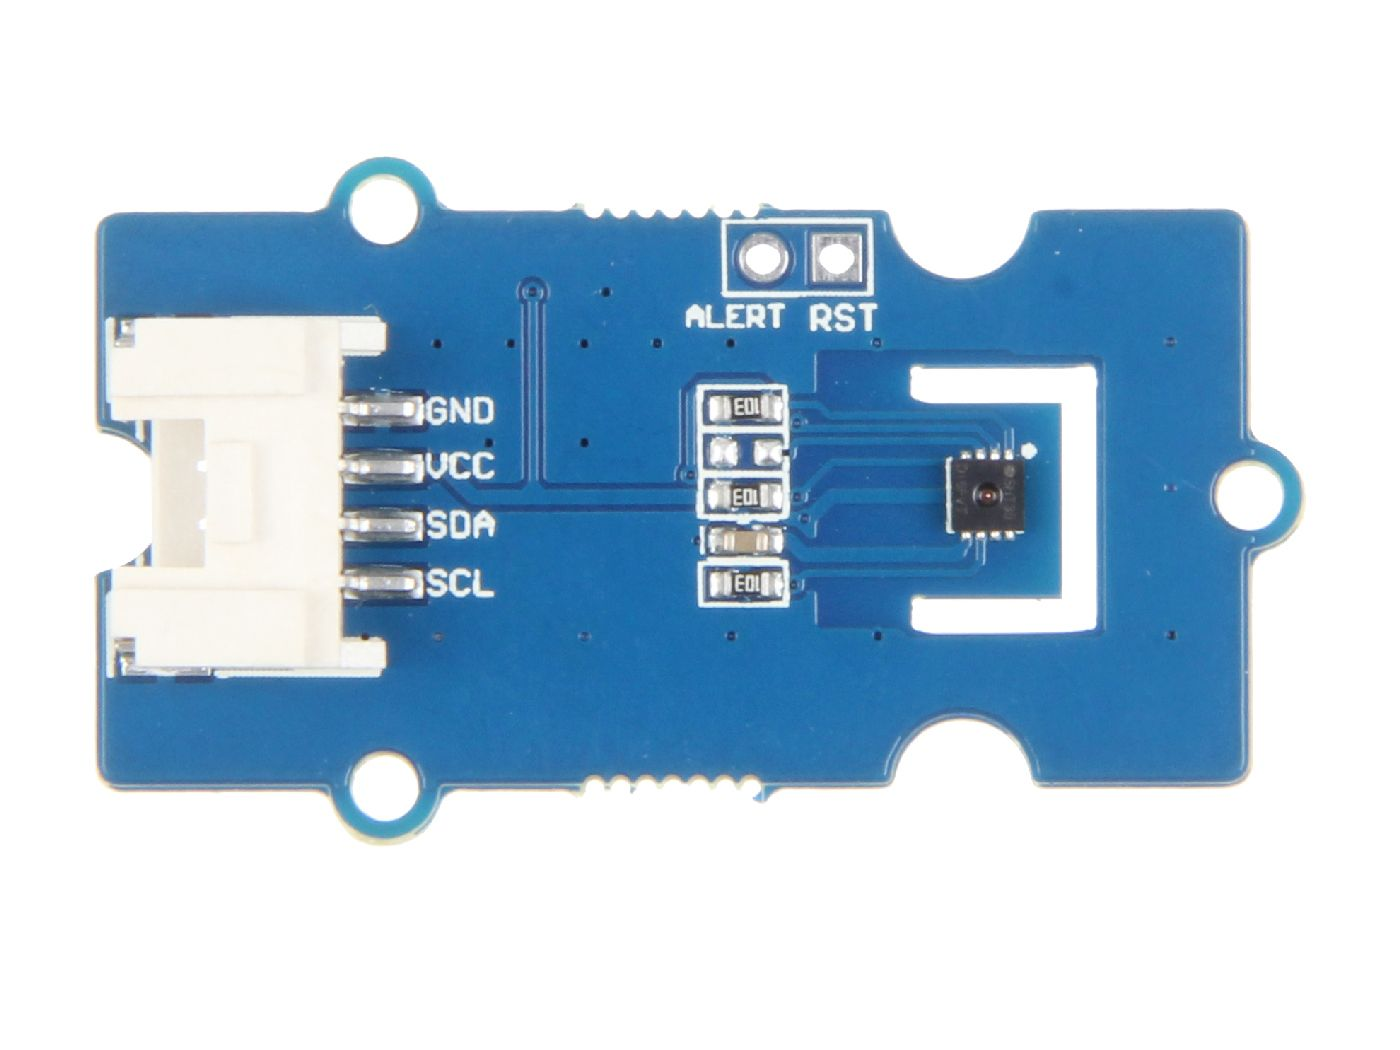
\includegraphics[width=\textwidth]{Images/sht35}
        \caption{SHT35 (Air conditions).}
        \label{fig:photo-sht35}
    \end{subfigure}
    \hfill
    \begin{subfigure}[b]{0.32\textwidth}
        \centering
        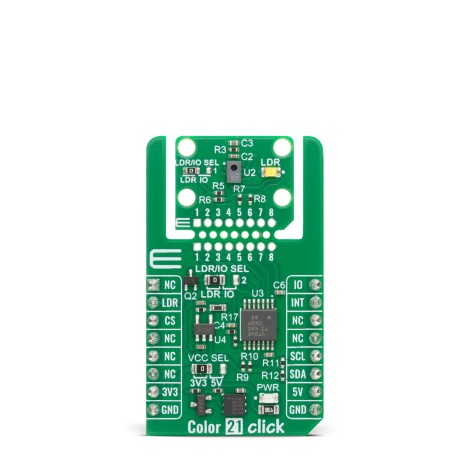
\includegraphics[width=\textwidth]{Images/tcs3448}
        \caption{TCS3448 (Light spectrum).}
        \label{fig:photo-tcs3448}
    \end{subfigure}
    \hfill
    \begin{subfigure}[b]{0.32\textwidth}
        \centering
        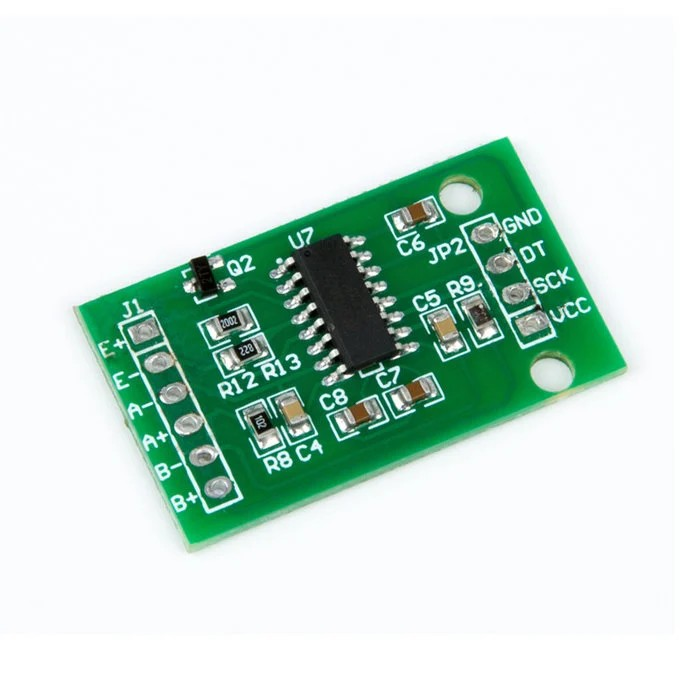
\includegraphics[width=\textwidth]{Images/hx711}
        \caption{HX711 (Plant mass).}
        \label{fig:photo-hx711}
    \end{subfigure}
    \caption[PhenoHive Core Sensor Suite]{The core numeric sensor suite of the PhenoHive station which were all selected for research-grade precision in an educational context.}
    \label{fig:sensor-photos}
\end{figure}
\section{Sensor calibration and metrological validation}

A raw sensor reading is of no use for phenotyping until it can be checked, trusted, and traced back to a known physical reference. In the context of an educational platform, this is particularly important because students need to be able to trust the data enough to reason about plant physiology and work with the collected data.Also, TAs need to be able to reproduce or check the calibration without any special expertise. The workflow I built answers both of these requirements by cross-referencing each sensor against traceable laboratory instruments at the WELCOME (Wallonia Electronics and Communications Measurements) lab \parencite{welcome-lab} and writing the resulting corrections straight into the station configuration.

\subsection{Calibration methodology}

The calibration procedure was done manually by using a steady-state reference sweep (Figure~\ref{fig:calibration-architecture}). The target conditions were adjusted directly on the reference laboratory instruments (the ESPEC climatic chamber and the monochromator combined with the optical setup) for each measurement setpoint. Once a stable and steady-state condition was reached, the reference values were recorded. 
At the same time, the raw readings from the studied sensor of the PhenoHive station was retrieved. By combining these reference measurements with the raw sensor outputs for each setpoint, a dataset was produced from which the calibration offsets and scaling factors were calculated. These offsets and scaling factors were then applied as correction values in the station's config file. This process ensured that each sensor's output was grounded in a known physical reference, allowing for accurate and reliable data collection during phenotyping experiments. 

\begin{figure}[H]
\centering
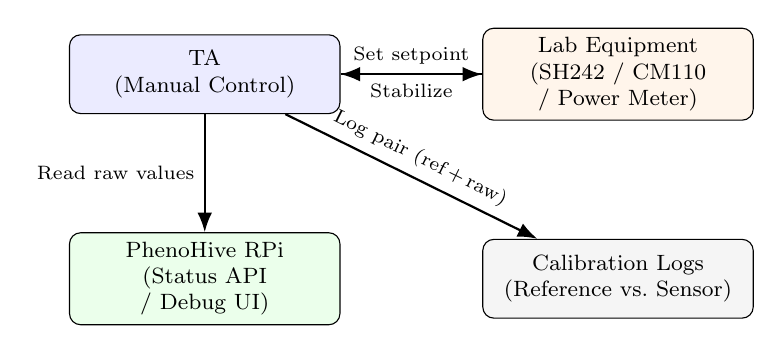
\begin{tikzpicture}[
    node distance=1.0cm and 1.8cm,
    block/.style={draw, rounded corners, align=center, text width=3.2cm, minimum height=1cm, fill=white, font=\footnotesize},
    arrow/.style={-{Latex[length=2.5mm]}, thick}
]
\node[block, fill=blue!8] (op) {TA\\(Manual Control)};
\node[block, fill=orange!8, right=of op] (eq) {Lab Equipment\\(SH242 / CM110 / Power Meter)};
\node[block, fill=green!8, below=1.5cm of op] (rpi) {PhenoHive RPi\\(Status API / Debug UI)};
\node[block, fill=gray!8, below=1.5cm of eq] (txt) {Calibration Logs\\(Reference vs.\ Sensor)};

\draw[arrow] (op) -- (eq) node[midway, above, font=\scriptsize] {Set setpoint};
\draw[arrow] (eq) -- (op) node[midway, below, font=\scriptsize] {Stabilize};
\draw[arrow] (op) -- (rpi) node[midway, left, font=\scriptsize] {Read raw values};
\draw[arrow] (op) -- (txt) node[midway, above, font=\scriptsize, sloped] {Log pair (ref\,+\,raw)};
\end{tikzpicture}
\caption[Manual Calibration Workflow]{Manual calibration workflow. Each setpoint was manually set on the reference equipment after which the raw sensor values were read after stabilization from the RPi API. Each logged calibration pair combines both the  reference instrument reading with the corresponding raw sensor output in orderto create the calibration dataset.}
\label{fig:calibration-architecture}
\end{figure}

Throughout the manual calibration the RPi kept on running as it normally would and was not put into a special calibration mode. This shows that the collected data is representative of the actual working conditions of the station.

In order to assist with the data collection, some lightweight Python scripts were used to continuously query the RPi's API. By comparing the live, raw outputs of the sensors against the stabilized laboratory equipment displays, the offsets and scaling factors were then calculated and written to the station's configuration file. 

\subsection{Environmental sensor calibration}
\label{sec:sht35-calibration}

The SHT35 temperature and humidity sensor was calibrated against an Espec SH-242 climatic chamber \parencite{espec-sh-242} which is a reference-grade instrument with active temperature and humidity regulation and factory-stated setpoint accuracies of $\pm0.3\,^\circ$C and $\pm3.0\,\%$\,RH (Figure \ref{fig:espec-sh242}). These reference accuracies set a floor on what this sweep can actually resolve. The SH-242's setpoint tolerances ($\pm0.3\,^\circ$C, $\pm3.0\,\%$\,RH) are in fact coarser than the SHT35's own datasheet accuracy ($\pm0.1\,^\circ$C, $\pm1.5\,\%$\,RH), so the exercise is best understood as a \emph{verification that the factory calibration still holds} rather than as a correction that improves on it: a chamber cannot certify a sensor to a tighter bound than its own uncertainty. The measured mean deviations ($+0.14\,^\circ$C, $-1.53\,\%$\,RH) are smaller in magnitude than the chamber's setpoint tolerance, which is the expected outcome of a sensor that agrees with the reference to within the reference's own uncertainty. The calibration followed a four-point corner sweep made to cover the extremes of the typical operating range. Two temperature levels (20$^\circ$C and 40$^\circ$C) were crossed-referenced with two humidity levels (40\% and $\approx$80\% RH). The chamber stabilized at 83\% RH rather than exactly 80\% at the 20$^\circ$C/high-humidity setpoint which is why that condition is reported as 83\% in the results. This choice of setpoints spans a bit more than the typical range for indoor plant experiments and captures both the offset and any temperature dependent drift in the humidity reading.

\begin{figure}[H]
    \centering
    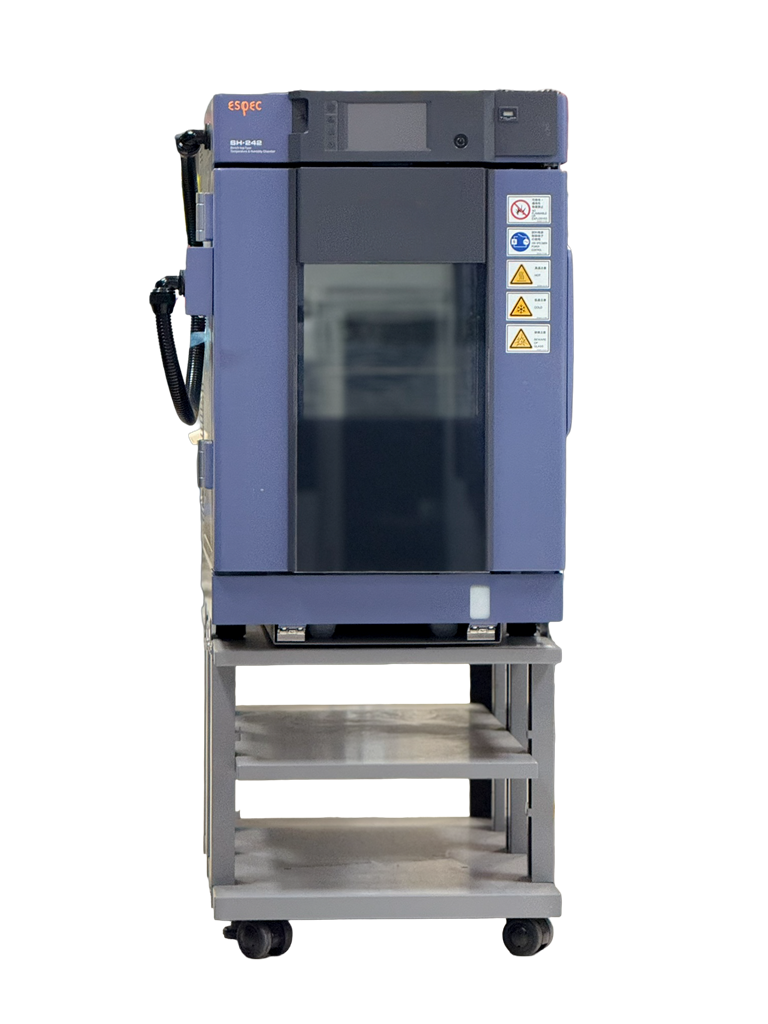
\includegraphics[width=0.5\textwidth]{Images/espec_sh242}
    \caption[Espec SH-242 Environmental Chamber]{The Espec SH-242 used for temperature and humidity sensor validation \parencite{espec-sh-242}.}
    \label{fig:espec-sh242}
\end{figure}

For each setpoint, the chamber was left for 15 minutes before the measurement was made in order for it to stabilize. 

\begin{table}[H]
\centering
\caption[SHT35 Calibration Results]{SHT35 calibration results against the SH242 climatic chamber. Each row corresponds to one stabilized setpoint. The error columns show the difference between the sensor reading and the chamber reference.}
\label{tab:sht35-calibration}
\small
\setlength{\tabcolsep}{5pt}
\renewcommand{\arraystretch}{1.25}
\begin{tabularx}{\textwidth}{|P{2.2cm}|X|X|X|X|}
\hline
\textbf{Setpoint} & \textbf{Ref.\ T ($^\circ$C)} & \textbf{SHT35 T ($^\circ$C)} & \textbf{Ref.\ RH (\%)} & \textbf{SHT35 RH (\%)} \\
\hline
20$^\circ$C / 40\% & 20.0 & 19.82 ($-$0.18) & 40.0 & 43.67 ($+$3.67) \\
\hline
20$^\circ$C / 83\% & 20.0 & 19.71 ($-$0.29) & 83.0 & 80.70 ($-$2.30) \\
\hline
40$^\circ$C / 40\% & 40.0 & 39.82 ($-$0.18) & 40.0 & 42.66 ($+$2.66) \\
\hline
40$^\circ$C / 80\% & 40.0 & 40.09 ($+$0.09) & 80.0 & 82.10 ($+$2.10) \\
\hline
\end{tabularx}
\vspace{0.4em}
{\footnotesize Mean corrections: $\Delta T = +0.14^\circ$C, $\Delta RH = -1.53$\%. Applied as linear corrections in \texttt{config.ini}.}
\end{table}

The results (Table~\ref{tab:sht35-calibration}) show that the temperature readings are stable across the entire range with deviations consistently below $\pm$0.3$^\circ$C. Humidity shows a slightly larger spread however. The sensor reads high at low humidity and low at high humidity. This is consistent with the accuracy characteristics documented in the sensor datasheet \parencite{sensirion-sht35}. The key metrological observation is that the deviations are small and consistent across the full operating range, which confirms that the sensor remains within its datasheet specification. The temperature deviation ($-0.14\,^\circ$C mean) sits below both the SHT35's own $\pm0.1\,^\circ$C accuracy and the chamber's $\pm0.3\,^\circ$C tolerance, so it cannot be distinguished from reference noise; the $+0.14\,^\circ$C correction is therefore applied conservatively and is not claimed to improve accuracy beyond the reference. Humidity shows a larger but repeatable trend (reading high at low RH), so the mean $-1.53\,\%$ offset is applied as a first-order linear compensation. With these corrections, the combined uncertainty stays within the bounds required for meaningful VPD-based transpiration analysis in the target operating range. Figure~\ref{fig:sht35-calibration-scatter} visualises the four calibration setpoints and the fitted mean offsets for both variables.

\begin{figure}[H]
\centering
\begin{subfigure}[b]{0.48\textwidth}
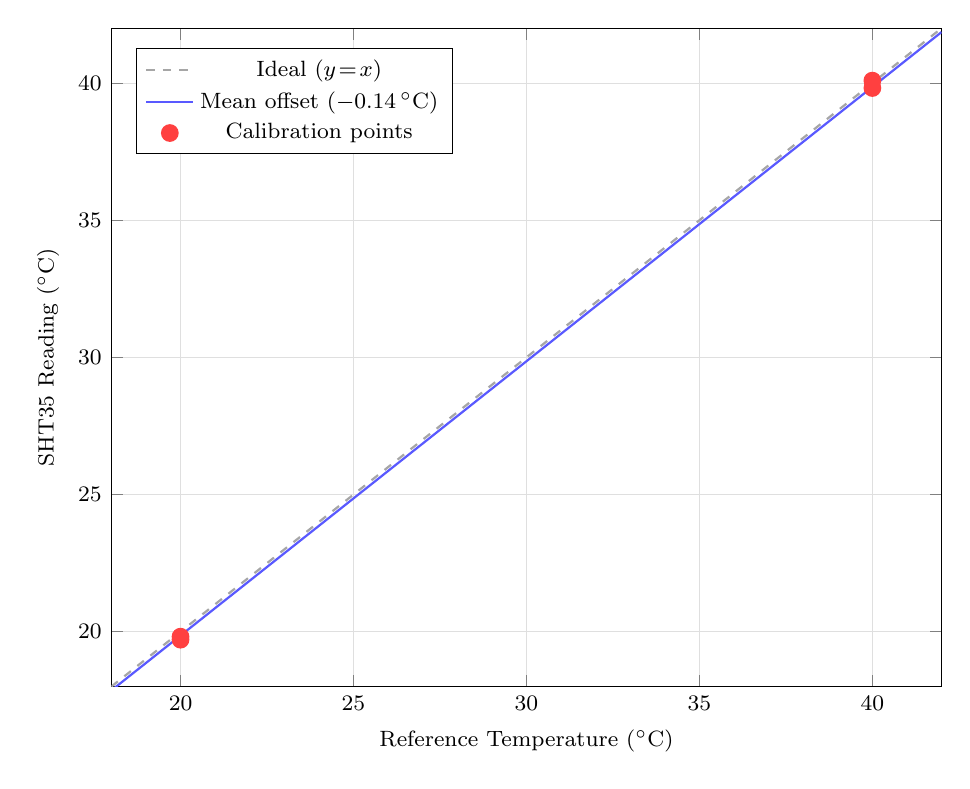
\begin{tikzpicture}
\begin{axis}[
    width=\textwidth,
    height=0.82\textwidth,
    xlabel={Reference Temperature ($^\circ$C)},
    ylabel={SHT35 Reading ($^\circ$C)},
    xmin=18, xmax=42,
    ymin=18, ymax=42,
    xtick={20,25,30,35,40},
    ytick={20,25,30,35,40},
    grid=both,
    grid style={line width=0.2pt, draw=gray!25},
    legend pos=north west,
    legend style={font=\footnotesize},
    tick label style={font=\footnotesize},
    label style={font=\footnotesize},
]
\addplot[domain=18:42, dashed, gray!70, thick] {x};
\addlegendentry{Ideal ($y\!=\!x$)}
\addplot[domain=18:42, blue!65, thick] {x - 0.14};
\addlegendentry{Mean offset ($-0.14\,^\circ$C)}
\addplot[only marks, mark=*, mark size=2.8pt, red!75, thick] coordinates {
    (20.0, 19.82) (20.0, 19.71) (40.0, 39.82) (40.0, 40.09)
};
\addlegendentry{Calibration points}
\end{axis}
\end{tikzpicture}
\caption{Temperature: consistent offset of $-0.14\,^\circ$C.}
\label{fig:sht35-temp-scatter}
\end{subfigure}
\hfill
\begin{subfigure}[b]{0.48\textwidth}
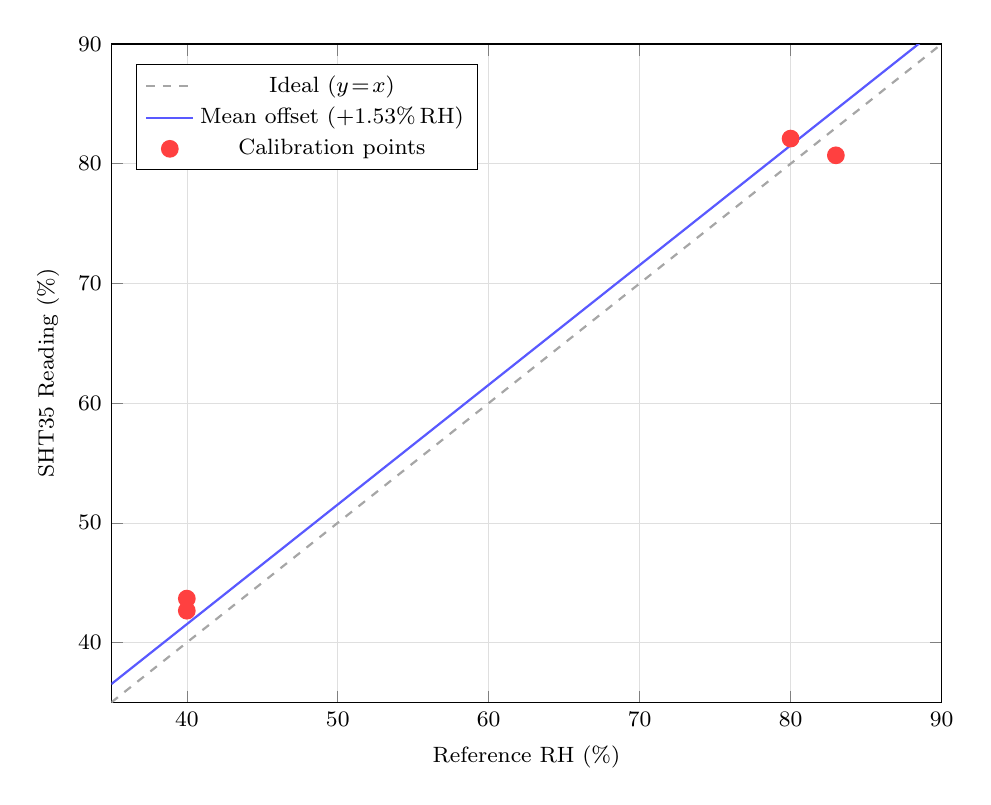
\begin{tikzpicture}
\begin{axis}[
    width=\textwidth,
    height=0.82\textwidth,
    xlabel={Reference RH (\%)},
    ylabel={SHT35 Reading (\%)},
    xmin=35, xmax=90,
    ymin=35, ymax=90,
    xtick={40,50,60,70,80,90},
    ytick={40,50,60,70,80,90},
    grid=both,
    grid style={line width=0.2pt, draw=gray!25},
    legend pos=north west,
    legend style={font=\footnotesize},
    tick label style={font=\footnotesize},
    label style={font=\footnotesize},
]
\addplot[domain=35:90, dashed, gray!70, thick] {x};
\addlegendentry{Ideal ($y\!=\!x$)}
\addplot[domain=35:90, blue!65, thick] {x + 1.53};
\addlegendentry{Mean offset ($+1.53$\%\,RH)}
\addplot[only marks, mark=*, mark size=2.8pt, red!75, thick] coordinates {
    (40.0, 43.67) (83.0, 80.70) (40.0, 42.66) (80.0, 82.10)
};
\addlegendentry{Calibration points}
\end{axis}
\end{tikzpicture}
\caption{Humidity: mean offset of $+1.53$\%\,RH with spread.}
\label{fig:sht35-humidity-scatter}
\end{subfigure}
\caption[SHT35 Calibration Scatter Plot]{SHT35 sensor readings put against the climatic chamber reference at the four calibration setpoints. The dashed diagonal represents what the perfect agreement would look like and the solid blue line is the fitted mean offset. Temperature behaviour is linear and consistent because all of the points fall within $\pm$0.3$^\circ$C of the offset line. The humidity points however show an increased residual spread across the range from $+3.67$\% at 40\%\,RH to $-2.30$\% at 83\%\,RH which indicates non-linearity that the single global correction ($-1.53$\%\,RH) doesn't fully capture.}
\label{fig:sht35-calibration-scatter}
\end{figure}

\clearpage
\subsection{Spectral sensor calibration}
\label{sec:tcs3448-calibration}

The TCS3448 spectral sensor was calibrated against a CM110 monochromator \parencite{oceanhood-monochromator} (the wavelength source) and combined with a reference power meter. The monochromator (Figure \ref{fig:monochromator-setup}) isolates a narrow-band wavelength from a broadband source and directs it toward the sensor, while the power meter provides a traceable irradiance reference at each wavelength step.

\begin{figure}[H]
    \centering
    \begin{subfigure}[b]{0.45\textwidth}
        \centering
        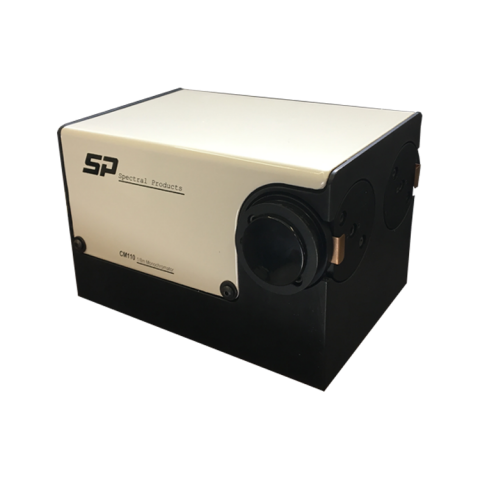
\includegraphics[width=\textwidth]{Images/monochromator_cm110}
        \caption{Oceanhood CM110 Monochromator.}
        \label{fig:monochromator}
    \end{subfigure}
    \hfill
    \begin{subfigure}[b]{0.45\textwidth}
        \centering
        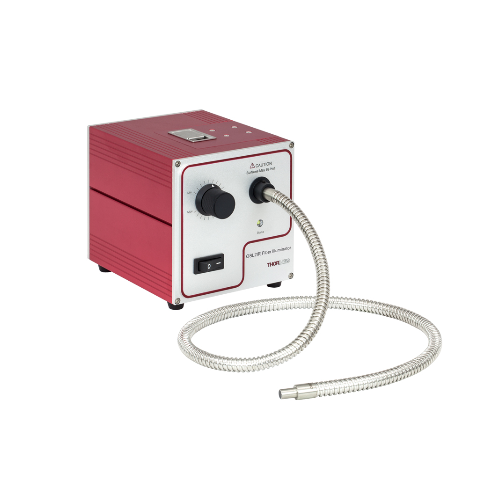
\includegraphics[width=\textwidth]{Images/light_source}
        \caption{Stabilized broadband light source.}
        \label{fig:light-source}
    \end{subfigure}
    
    \vspace{0.5em}
    \begin{subfigure}[b]{0.45\textwidth}
        \centering
        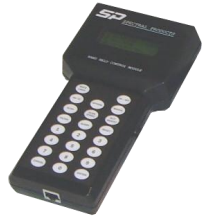
\includegraphics[width=\textwidth]{Images/CM1210}
        \caption{CM1210 Monochromator Controller.}
        \label{fig:cm1210-controller}
    \end{subfigure}
    \hfill
    \begin{subfigure}[b]{0.45\textwidth}
        \centering
        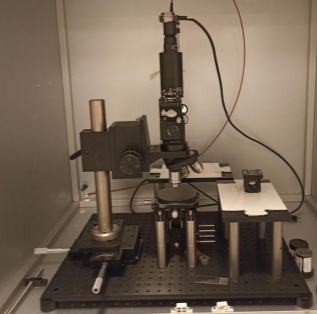
\includegraphics[width=\textwidth]{Images/optosetup}
        \caption{Full optical calibration bench setup.}
        \label{fig:opto-setup}
    \end{subfigure}
    \caption[Spectral Calibration Setup at the WELCOME Lab]{The spectral calibration setup at the WELCOME lab, including the monochromator for wavelength isolation, the power meter, the stabilized light source and the test bench configuration \parencite{oceanhood-monochromator, welcome-lab}.}
    \label{fig:monochromator-setup}
\end{figure}

The sweep ran from 300\,nm to 940\,nm in 20\,nm steps. It needed two diffraction gratings as per the test bench configuration. Grating~1 (2400\,G/mm, blaze 240\,nm) handled 300--680\,nm, and Grating~2 (1200\,G/mm, blaze 750\,nm) handled 600--940\,nm. A grating fans broadband light out into its separate wavelengths. The groove density sets how finely it resolves them, and the blaze angle tilts the diffraction efficiency toward a peak at the design wavelength, which is what keeps the signal-to-noise ratio high across the sweep. At each step I logged the monochromator output power on the reference power meter and, at the time, read the TCS3448 raw counts from the RPi API using the simple script.

The sweep showed that the empirical peak wavelengths of the visible TCS3448 channels (F1--F7) sit consistently below the typical values listed in the manufacturer datasheet \parencite{ams-osram-tcs3448}, by about 25\,nm on average (individual channels range from $\sim$16\,nm to $\sim$37\,nm). The empirical peaks of F8 (datasheet typical 748\,nm) and NIR (datasheet typical 855\,nm) fall well within the 20\,nm resolution of the sweep of their datasheet values, showing no comparable offset. Two non-exclusive mechanisms can explain the visible-channel offset. The first is a normal sensor property which is the manufacturing-lot variation. The second is a that a near-uniform offset across all visible channels also indicates a small systematic wavelength-calibration offset in the monochromator itself. The current single benchmarking data cannot fully separate the two causes. Resolving this issue would demand an independent wavelength reference such as a calibrated spectral line source, identified as future work in Section~\ref{sec:future-work}. For the platform's current single-station use the practical impact is limited: the offset is consistent and repeatable, so within a given station the channel ordering and the relative spectral structure are preserved (Figure~\ref{fig:tcs3448-comparison}). The distinction is not irrelevant, however, for \emph{absolute} wavelength labelling: if the shift originates in the monochromator rather than the sensor, the sensor's true peaks remain near the datasheet values and the empirical mapping would mislabel them by about 25\,nm. Settling this requires an independent wavelength reference or a per-station sweep, both identified as future work in Section~\ref{sec:future-work}. With that caveat, the offset is encompassed by the empirical channel mapping, derived from the wavelengths where each channel showed its maximum response. This is summarized in Table~\ref{tab:tcs3448-channel-mapping} and used throughout the platform.

\begin{figure}[H]
    \centering
    \begin{subfigure}[b]{0.48\textwidth}
        \centering
        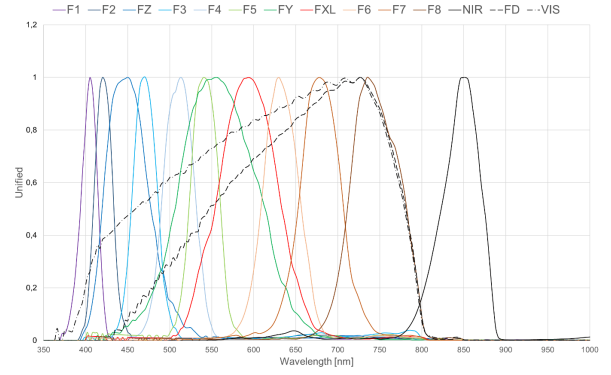
\includegraphics[width=\textwidth]{Images/tcs3448wavelengths}
        \caption{Theoretical responsivity. \textcopyright\ ams-OSRAM AG, reproduced from the TCS3448 datasheet for academic comparison \parencite{ams-osram-tcs3448}.}
        \label{fig:tcs3448-datasheet-wavelengths}
    \end{subfigure}
    \hfill
    \begin{subfigure}[b]{0.48\textwidth}
    \centering
    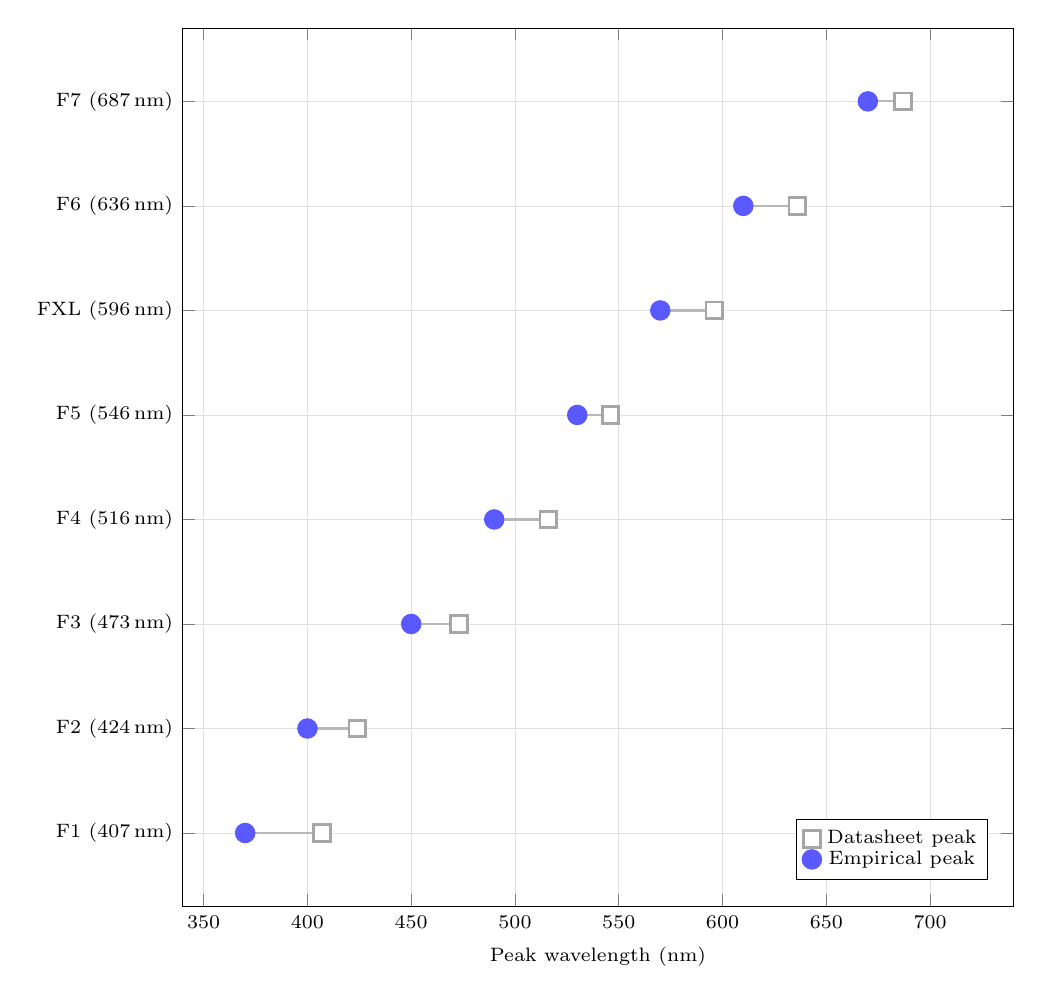
\begin{tikzpicture}
    \begin{axis}[
        width=\textwidth,
        height=1.05\textwidth,
        xlabel={Peak wavelength (nm)},
        xmin=340, xmax=740,
        ymin=0.3, ymax=8.7,
        xtick={350,400,450,500,550,600,650,700},
        ytick={1,2,3,4,5,6,7,8},
        yticklabels={%
            F1 (407\,nm),
            F2 (424\,nm),
            F3 (473\,nm),
            F4 (516\,nm),
            F5 (546\,nm),
            FXL (596\,nm),
            F6 (636\,nm),
            F7 (687\,nm)},
        grid=both,
        grid style={line width=0.2pt, draw=gray!25},
        tick label style={font=\scriptsize},
        label style={font=\scriptsize},
        legend pos=south east,
        legend style={font=\scriptsize, inner sep=2pt, row sep=-3pt},
    ]
    % Connecting lines (shift arrows)
    \addplot[gray!55, thick, forget plot] coordinates {(370,1)(407,1)};
    \addplot[gray!55, thick, forget plot] coordinates {(400,2)(424,2)};
    \addplot[gray!55, thick, forget plot] coordinates {(450,3)(473,3)};
    \addplot[gray!55, thick, forget plot] coordinates {(490,4)(516,4)};
    \addplot[gray!55, thick, forget plot] coordinates {(530,5)(546,5)};
    \addplot[gray!55, thick, forget plot] coordinates {(570,6)(596,6)};
    \addplot[gray!55, thick, forget plot] coordinates {(610,7)(636,7)};
    \addplot[gray!55, thick, forget plot] coordinates {(670,8)(687,8)};
    % Datasheet peaks (hollow squares)
    \addplot[only marks, mark=square*, mark size=3pt,
             mark options={fill=white, draw=gray!70, line width=1pt}] coordinates {
        (407,1)(424,2)(473,3)(516,4)(546,5)(596,6)(636,7)(687,8)
    };
    \addlegendentry{Datasheet peak}
    % Empirical peaks (filled circles)
    \addplot[only marks, mark=*, mark size=3.5pt, blue!65] coordinates {
        (370,1)(400,2)(450,3)(490,4)(530,5)(570,6)(610,7)(670,8)
    };
    \addlegendentry{Empirical peak}
    \end{axis}
    \end{tikzpicture}
        \caption{Empirical peak wavelengths from the monochromator sweep vs.\ the datasheet's nominal values. Each row shows one channel where the circle is what's the measured empirical peak and the square is what's the datasheet value. The horizontal gap is the shift of the visible channels. They range from $\sim$16\,nm (F5) to $\sim$37\,nm (F1), with a mean of about 25\,nm. F8 and NIR are not displayed because they aligned with their datasheet peaks within the sweep resolution.}
        \label{fig:tcs3448-empirical-response}
    \end{subfigure}
    \caption[TCS3448 Spectral Channel Peak Wavelengths: Datasheet vs.\ Empirical]{Comparison between nominal peak wavelengths from the TCS3448 datasheet and the empirical peaks determined by the monochromator sweep.}
    \label{fig:tcs3448-comparison}
\end{figure}

\clearpage
\begin{table}[htbp]
\centering
\caption[TCS3448 Empirical Channel Peak Wavelengths]{Empirical peak wavelengths of the TCS3448 channels measured by the monochromator sweep. The ``Empirical peak'' column reflects the wavelength range at which the channel registered its highest raw count during the sweep (Grating~1 was used for channels peaking below 680\,nm, and Grating~2 for channels peaking above 680\,nm).}
\label{tab:tcs3448-channel-mapping}
\small
\setlength{\tabcolsep}{5pt}
\renewcommand{\arraystretch}{1.25}
\begin{tabularx}{\textwidth}{|P{1.5cm}|X|X|P{4.5cm}|}
\hline
\textbf{Channel} & \textbf{Datasheet peak (nm)} & \textbf{Empirical peak (nm)} & \textbf{Dominant response range} \\
\hline
F1 & 407 & $\sim$360--380 & UV/Violet \\
\hline
F2 & 424 & $\sim$400 & Violet \\
\hline
F3 & 473 & $\sim$440--460 & Blue \\
\hline
F4 & 516 & $\sim$480--500 & Cyan/Green \\
\hline
F5 & 546 & $\sim$520--540 & Green \\
\hline
FXL & 596 & $\sim$560--580 & Yellow/Orange \\
\hline
F6 & 636 & $\sim$600--620 & Orange/Red \\
\hline
F7 & 687 & $\sim$660--680 & Red \\
\hline
F8 & 748 & $\sim$720--760 & Far Red / NIR edge \\
\hline
NIR & 855 & $\sim$840--900 & Near-Infrared \\
\hline
\end{tabularx}

\vspace{0.4em}
\end{table}

The complete calibration state applied to the physical station is stored in \texttt{config.ini}. Table~\ref{tab:tcs3448-calibration-state} lists the values as deployed in each station.

\begin{table}[H]
\centering
\caption[TCS3448 Deployed Calibration State]{Deployed TCS3448 calibration state as stored in \texttt{config.ini} on the station. Scale factor converts raw ADC counts to calibrated irradiance (mW/m$^2$) after dark subtraction. The dark offset is the residual count observed with the sensor fully covered.}
\label{tab:tcs3448-calibration-state}
\small
\setlength{\tabcolsep}{5pt}
\renewcommand{\arraystretch}{1.2}
\begin{tabularx}{\textwidth}{|P{1.6cm}|X|X|P{4.5cm}|}
\hline
\textbf{Channel} & \textbf{Scale factor} & \textbf{Dark offset (counts)} & \textbf{Empirical peak (nm)} \\
\hline
F1   & 0.880 & 0 & $\sim$360--380 \\
\hline
F2   & 0.864 & 0 & $\sim$400 \\
\hline
F3   & 1.063 & 0 & $\sim$440--460 \\
\hline
F4   & 1.085 & 0 & $\sim$480--500 \\
\hline
F5   & 2.90  & 0 & $\sim$520--540 \\
\hline
F6   & 9.81  & 1 & $\sim$600--620 \\
\hline
F7   & 9.68  & 2 & $\sim$660--680 \\
\hline
F8   & 9.21  & 2 & $\sim$720--760 \\
\hline
FZ   & 0.96  & 0 & Broad (CIE Z tristimulus) \\
\hline
FY   & 2.0   & 0 & Broad (CIE Y / luminance) \\
\hline
FXL  & 2.36  & 0 & $\sim$560--580 (empirical) \\
\hline
NIR  & 11.54 & 4 & $\sim$840--900 \\
\hline
\texttt{2x\_vis\_1} & 1.0 (uncal.) & 2 & Broadband visible \\
\hline
\texttt{fd\_1}      & 1.0 (uncal.) & 79 & AC-coupled (flicker) \\
\hline
\end{tabularx}
\end{table}

From the sweep data (Table~\ref{tab:tcs3448-sweep-excerpt}), a per-channel scaling factor was computed by combining the power-to-count ratio from the sweep with a normalization to spectral irradiance:
\begin{equation}
    s_k = \frac{P_{\text{ref},k}}{C_{\text{peak},k}} \cdot \frac{10^{-3}}{A_{\text{eff}}}
    \label{eq:tcs-scale}
\end{equation}
where $P_{\text{ref},k}$ [$\mu$W] is the optical power measured by the reference power meter at the wavelength of peak response for channel $k$, $C_{\text{peak},k}$ is the corresponding peak ADC count from the calibration sweep, and $A_{\text{eff}} \approx 7.0 \times 10^{-8}$\,m$^2$ is the effective per-channel optical aperture area according to the TCS3448 datasheet \parencite{ams-osram-tcs3448}. The $10^{-3}$ factor is what converts µW to mW. These factors convert raw ADC counts directly into spectral irradiance in mW/m$^2$, a range (typically 10--5000\,$\text{mW/m}^2$ per channel under indoor lighting) that is human-readable on the dashboard and matches the conventions used for photosynthetically active radiation (PAR) measurements.

\begin{table}[H]
\centering
\caption[TCS3448 Grating 1 Sweep Results (Excerpt)]{Sweep results on Grating~1 for selected channels. For each monochromator wavelength, the power meter reference and the dominant TCS3448 channel response are shown. Channels not listed peaked below the noise floor at the given wavelength.}
\label{tab:tcs3448-sweep-excerpt}
\small
\setlength{\tabcolsep}{4pt}
\renewcommand{\arraystretch}{1.2}
\begin{tabularx}{\textwidth}{|P{1.8cm}|X|X|X|}
\hline
\textbf{$\lambda$ (nm)} & \textbf{Ref. power} & \textbf{Peak channel} & \textbf{Peak counts} \\
\hline
380 & 0.333\,$\mu$W & F1 & 5\,404 \\
\hline
400 & 0.471\,$\mu$W & F2 & 7\,781 \\
\hline
440 & 0.826\,$\mu$W & F3 & 10\,121 \\
\hline
480 & 1.220\,$\mu$W & F4 & 14\,184 \\
\hline
500 & 1.319\,$\mu$W & F4 & 17\,364 \\
\hline
520 & 1.584\,$\mu$W & F5 & 7\,782 \\
\hline
560 & 2.006\,$\mu$W & FXL & 10\,625 \\
\hline
600 & 2.222\,$\mu$W & F6 & 13\,397 \\
\hline
620 & 2.205\,$\mu$W & F6 & 24\,225 \\
\hline
640 & 2.205\,$\mu$W & F6 & 17\,677 \\
\hline
660 & $2.115\,\mu$W & F7 & 21\,720 \\
\hline
680 & $2.031\,\mu$W & F7 & 20\,502 \\
\hline
\end{tabularx}

\vspace{0.4em}
\end{table}

A second calibration step addressed the sensor's electrical noise floor. Even in complete darkness, each channel produces a small number of counts due to some noise in the silicon photodiodes. These dark counts vary by channel. Longer-wavelength channels (F7, F8, NIR) exhibit higher noise than the visible-range channels. The dark baseline was measured by physically covering the sensor and recording the residual counts. Per-channel offsets were then subtracted before the irradiance scaling is applied, so the station reports exactly zero under no-light conditions.

During the second grating sweep (Grating 2, 600--940\,nm), the grating's higher power output pushed multiple channels into the 16-bit ADC ceiling of 65\,535 counts. Those points were saturated so they were dropped from the coefficient calculation. The 600--680\,nm overlap between the two gratings is used as a sanity check. I observed that each channel that peaked at a given wavelength peaked there under both gratings which confirms the channel mapping. Because the saturated peak samples were discarded, the long-wavelength scale factors (F6--F8, NIR) were computed from the largest \emph{unsaturated} counts available rather than from the true peak counts; this is why their factors in Table~\ref{tab:tcs3448-calibration-state} are several times larger than the visible-channel factors and cannot be reproduced directly from the unsaturated Grating~1 counts shown in the excerpt of Table~\ref{tab:tcs3448-sweep-excerpt}.

Everything the calibration produces is in \texttt{config.ini}. Recalibrating, if need be, only requires editing one flat file and restarting the service, with no code changes at all.

The same precision to accuracy split observed on the SHT35 shows up again here. The TCS3448 channels are precise and under steady light their responses are consistent and repeatable. The systematic wavelength shift is an accuracy problem, there's a fixed gap between where each channel is supposed to peak and where it actually does. The empirical channel mapping and the per-channel scaling factors from the monochromator sweep cancel that gap, so accuracy is restored without touching the sensor's underlying precision.

\paragraph{Measurement uncertainty.}
The 20\,nm sweep increments restrict each channel's peak wavelength to about $\pm10\,$nm. This uncertainty is fine for the broad visible channels (F1--F7) but becomes less ideal for the narrower long-wavelength ones (F8, NIR). The power meter's own accuracy rating also contributes to the scaling-factor uncertainty.

\clearpage
\subsection{Scale and camera calibration}

The load cell and HX711 ADC were carried over from \textcite{colinet2025}, who already showed they are adequate for evapotranspiration tracking on PhenoHive, so I ran no full lab sweep on them. The inherited two-point procedure is the right amount of effort for a teaching station. The tare value, the zero-load ADC reading, is taken with an empty platform, and the calibration factor comes from one known mass placed on the scale. Both numbers go into \texttt{config.ini} and are applied at read time. A dashboard wizard on the DebugUI webpage steps the TA through the two actions, which cuts down on slip-ups during deployment.

The platform now reports the plant's growth in real-world units instead of just a plain pixel count which is hard to interpret. For correct calibration, the TA sets a \texttt{pixel\_to\_cm\_ratio} through a semi-automated step where an object of known size sits in the field of view. The system then applies that ratio to its skeleton-length figure which means that students can read growth in centimeters. The station can also capture a background image on demand which gives it a clean reference for shadow removal and background subtraction that sharpens the morphological measurements. This was retained from the previous version of the platform, but the calibration step was made more user-friendly by integrating it into the DebugUI.

\section{Data gathering and signal processing}

PhenoHive has to turn physical measurements into biological indicators a student can trust. This means that data quality is the whole point here. If there's too much noise, the students start doubting the readings instead of studying plant physiology. My work therefore went into two things. First, a standard way to integrate sensors and second, a two-stage MAD filter pipeline that cleans and aggregates the raw signals before they reach storage and visualization.

\subsection{Data smoothing and noise rejection}
\label{sec:data-smoothing}

Raw sensor data can contain sudden spikes from electrical interference, I$^2$C bus jitter or physical disturbances to the scale. The pipeline applies Median Absolute Deviation (MAD) filtering \parencite{leys2013mad} at two stages to reject outliers before they reach the stored record. For a set of $n$ values, the filter computes the median $\tilde{x}$ and discards any value that satisfies the condition:
\begin{equation}
    |x_i - \tilde{x}| > k \cdot \text{MAD}, \qquad \text{where } \text{MAD} = \text{median}(|x_i - \tilde{x}|)
\end{equation}
with sensitivity factor $k = 3$ by default (configurable). At least three samples are needed for meaningful outlier detection.

\textbf{Stage~1 — burst-level.} A sensor is read $n$ times within one collection event and those reads are filtered even before they become a collection record (Figure~\ref{fig:burst-pipeline}). This allows for fine-grained spike rejection in noisy deployments.

\textbf{Stage~2 — cross-collection.} At the close of each publish window, the five records that were gathered over 600\,s all pass through the same MAD filter and are then averaged into the one single record that's then persisted locally and forwarded to InfluxDB (Figure~\ref{fig:two-tier-timing}). 

\begin{figure}[H]
\centering
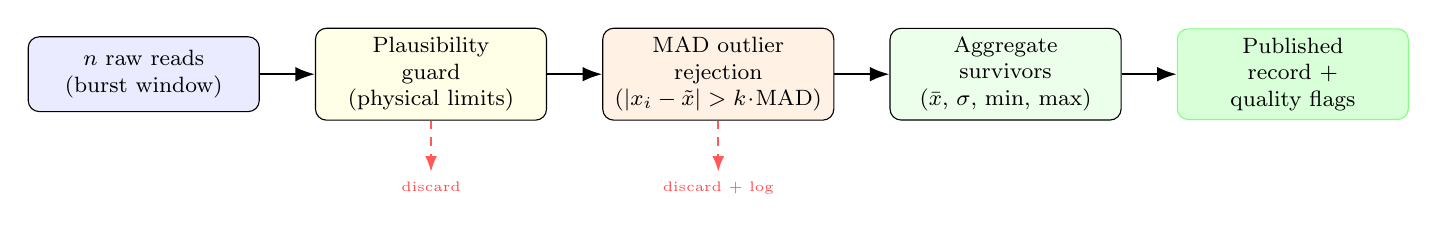
\begin{tikzpicture}[
    node distance=0.5cm and 0.7cm,
    stage/.style={draw, rounded corners, align=center, text width=2.7cm,
        minimum height=0.95cm, font=\footnotesize, fill=white},
    arrow/.style={-{Latex[length=2.5mm]}, thick},
    redarrow/.style={-{Latex[length=2mm]}, dashed, red!65, thick}
]
\node[stage, fill=blue!8]    (burst) {$n$ raw reads\\(burst window)};
\node[stage, fill=yellow!10, right=of burst]  (plaus) {Plausibility\\guard\\(physical limits)};
\node[stage, fill=orange!10, right=of plaus]  (mad)   {MAD outlier\\rejection\\($|x_i-\tilde{x}|>k\!\cdot\!\mathrm{MAD}$)};
\node[stage, fill=green!8,   right=of mad]    (agg)   {Aggregate\\survivors\\($\bar{x}$, $\sigma$, min, max)};
\node[stage, fill=green!15, draw=green!50, right=of agg] (pub) {Published\\record +\\quality flags};

\draw[arrow] (burst) -- (plaus);
\draw[arrow] (plaus) -- (mad);
\draw[arrow] (mad)   -- (agg);
\draw[arrow] (agg)   -- (pub);

\draw[redarrow] (plaus.south) -- ++(0,-0.65)
    node[below, font=\tiny, red!70] {discard};
\draw[redarrow] (mad.south)   -- ++(0,-0.65)
    node[below, font=\tiny, red!70] {discard + log};
\end{tikzpicture}
\caption[Burst Sampling and Signal Processing Pipeline]{Per-collection signal processing pipeline. Each collection event makes $n$ raw sensor reads where the values that are outside of physical plausibility bounds are immediately discarded. The MAD filter then removes each statistical outlier from the remaining burst. This means that the surviving samples are all aggregated into one smoothed value with quality metadata appended for storage and display.}
\label{fig:burst-pipeline}
\end{figure}

Figure~\ref{fig:mad-filtering} shows the cleaning effect on a real temperature trace. Before the MAD filtering stage, the plausibility guards throw out physically impossible values, such as humidity outside 0--100\,\% or negative illuminance, and logs them as invalid readings.

\begin{figure}[H]
    \centering
    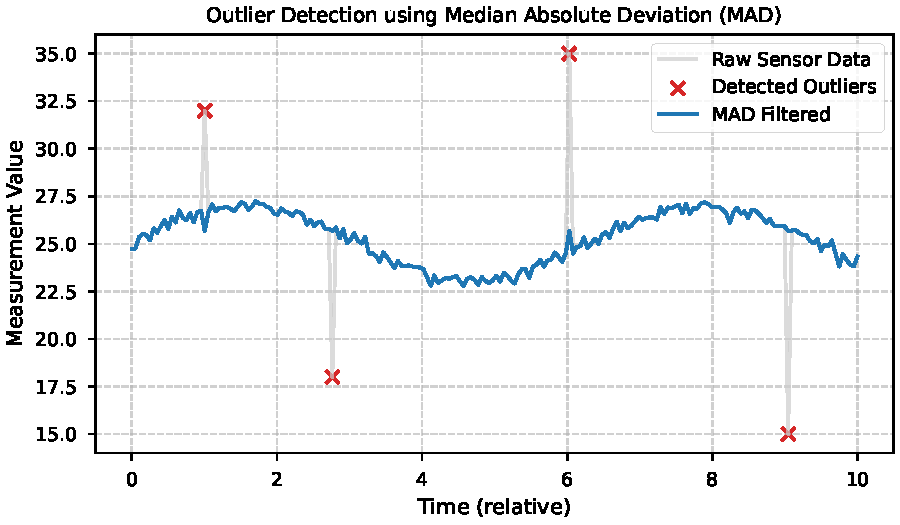
\includegraphics[width=0.85\textwidth]{Images/mad_filtering}
    \caption[Signal Cleaning Using MAD Filtering]{Signal cleaning using Median Absolute Deviation (MAD). This two-stage pipeline identifies and removes anytransient spikes that are caused by electrical interference or physical disturbances. This prevents them from corrupting any long-term trend analysis.}
    \label{fig:mad-filtering}
\end{figure}

\subsection{Confidence flags and quality metadata}

When publishing the aggregated record, the system does not only output a single smoothed value. It also includes statistical indicators of the signal's stability over the window, such as the minimum, maximum and standard deviation.
Each sensor reading is also tagged with confidence metadata. The system tracks the ratio of successful reads to attempted reads and computes the coefficient of variation (CV) within the burst:
\begin{equation}
    CV = \frac{\sigma}{\mu}
\end{equation}
where the sample mean $\mu$ and sample standard deviation $\sigma$ are calculated by the acquisition pipeline from the set of valid, post-filtering samples collected during the burst window. If the success ratio goes below a configured threshold or the $CV$ exceeds the maximum allowed variation, the record is then flagged with a \texttt{low\_confidence} marker.

\subsection{Acquisition summary}

Taken together, the acquisition layer pulls back from a hardware-first view. It hides the hardware specifics, filters out physical noise, and holds every channel to a calibration that traces back to laboratory references.

After calibration, the temperature reading is verified to agree with the reference chamber to within its $\pm$0.3$^\circ$C setpoint tolerance, with the SHT35's own datasheet accuracy ($\pm$0.1$^\circ$C) remaining the limiting figure. The humidity measurement holds around $\pm$2.2\,\% RH across the usual 40--80\,\% indoor range. The Spectral channels now are now mapped to physical irradiance units with per-channel dark subtraction. This means that what reaches the student is data they is ready to be read and interpreted biologically.


\chapter{Storage, visualization and access control}
\label{ch:storage}

Two constraints drive the storage and access-control design. The edge nodes run unattended in student homes and face unstable connectivity conditions, so local storage must work independently of network availability. All twenty stations write to the same InfluxDB instance, so the schema must enforce per-group isolation at the query level, not just at the dashboard level. This chapter describes both these things. The local-first persistence model on the edge side, and the InfluxDB schema and multi-tenant access-control model on the server side.

\section{Edge storage and local caching}

The edge runtime keeps two copies. Every measurement first goes into local storage before the station ever tries to push it upstream, so a network outage cannot lose data. This follows the local-buffer pattern that production IoT systems use wherever connectivity is unstable \parencite{ruralegehealth2026}.

\subsection{Flat-file CSV logging}

On the actual device, the long term backup solution is a simple csv file used as a log. The \texttt{DataManager} python script is what appends each measurement row to the file. Picking CSV over a local SQLite database was intentional. If a power cut interrupts a write, it can corrupt the database file. And to read a CSV you can just insert the SD card into any computer, with no database tooling or special knowledge in the way.

\subsection{Offline JSONL caching queue}

When the central InfluxDB is offline or unreachable, the device has to buffer its data so none is lost. Because of the fact that an in-memory queue would vanish on power loss, the station instead keeps a persistent retry queue in \textbf{JSON Lines (JSONL)} format at \texttt{/opt/phenohive/data/offline\_queue.jsonl}.

A plain JSON array would need rewriting on every addition which is why a JSONL file was used. This is because it just appends each new record as one line so this means that the write cost stays flat however long the queue grows.

\subsection{Synchronization protocol}

The data lifecycle follows the state machine in Figure~\ref{fig:edge-sync-flow}. A new measurement first goes to the local csv file, then to InfluxDB if it's available. If that push fails, then the record is appended to the offline queue and is retried after the next aquisition cycle. This keeps it out of a busy-retry loop which could block the system. On a successful push however, the entire backlog is flushed out in one pass, and the queue now will only contain the valid records that couldn't be pushed.

\begin{figure}[H]
\centering
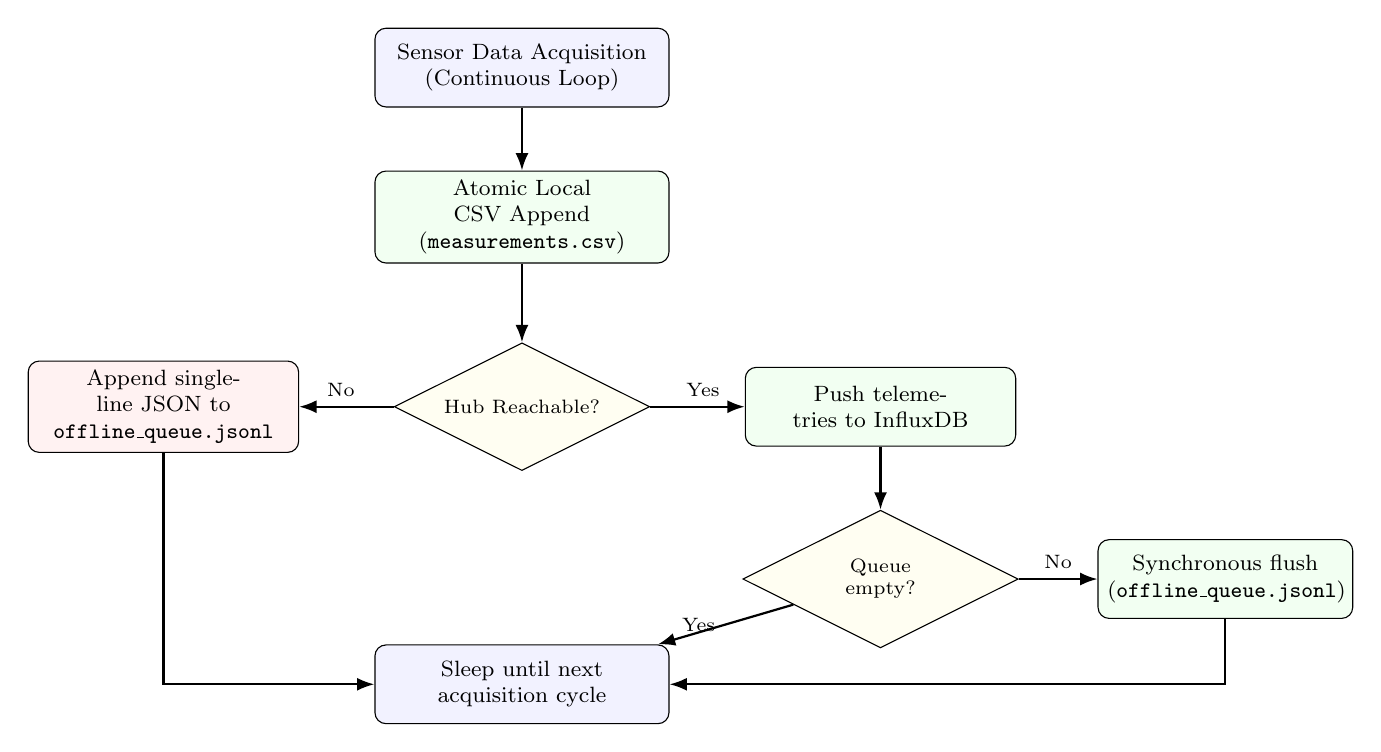
\begin{tikzpicture}[
    node distance=1.3cm and 0.8cm,
    block/.style={draw, rounded corners, align=center, text width=3.5cm, minimum height=1.0cm, fill=white, font=\footnotesize},
    decision/.style={draw, diamond, aspect=2, align=center, text width=2.2cm, fill=white, font=\scriptsize},
    arrow/.style={-{Latex[length=2.2mm]}, thick}
]
% Nodes
\node[block, fill=blue!5] (acquire) {Sensor Data Acquisition\\(Continuous Loop)};
\node[block, fill=green!5, below=0.8cm of acquire] (csv) {Atomic Local CSV Append\\(\texttt{measurements.csv})};
\node[decision, fill=yellow!5, below=1.0cm of csv] (net) {Hub Reachable?};
\node[block, fill=green!5, right=1.2cm of net, text width=3.2cm] (push) {Push telemetries to InfluxDB};
\node[decision, fill=yellow!5, below=0.8cm of push, text width=1.8cm] (queue) {Queue\\empty?};
\node[block, fill=green!5, right=1.0cm of queue, text width=3.0cm] (flush) {Synchronous flush\\(\texttt{offline\_queue.jsonl})};
\node[block, fill=red!5, left=1.2cm of net, text width=3.2cm] (buffer) {Append single-line JSON to \texttt{offline\_queue.jsonl}};
\node[block, fill=blue!5, below=2.2cm of net] (sleep) {Sleep until next acquisition cycle};

% Arrows
\draw[arrow] (acquire) -- (csv);
\draw[arrow] (csv) -- (net);
\draw[arrow] (net) -- node[above, font=\scriptsize, xshift=2pt] {Yes} (push);
\draw[arrow] (net) -- node[above, font=\scriptsize, xshift=-2pt] {No} (buffer);
\draw[arrow] (push) -- (queue);
\draw[arrow] (queue) -- node[left, font=\scriptsize] {Yes} (sleep);
\draw[arrow] (queue) -- node[above, font=\scriptsize] {No} (flush);
\draw[arrow] (flush) |- (sleep);
\draw[arrow] (buffer) |- (sleep);

\end{tikzpicture}
\caption[Edge Node Data Synchronization Flow]{Edge node data synchronization flow. Acquired readings are immediately logged to local flat-file CSV for physical resilience, then routed depending on the state of the network connectivity. Unsent records are written to a persistent JSONL queue file and flushed out on connection restoration.}
\label{fig:edge-sync-flow}
\end{figure}

\section{Central database schema and cardinality control}

On the server, InfluxDB handles the centralized time-series storage \parencite{influxdb-docs}. Instead of using tables like a relational database, it lays points out along a time axis, which is a good fit for the high-frequency concurrent writes and time-range queries a fleet of stations throws at it. This choice is carried over from previous theses as it was deemed to still be the best fit for the use case, and it has proven to be robust and performant in practice.

\subsection{Database schema layout}

All PhenoHive telemetry is stored inside a single InfluxDB bucket named \texttt{phenohive} under a unified measurement called \texttt{phenohive\_measurements}. To optimize indexing and search speeds, the points are organized into tags (which are indexed by InfluxDB's Time Series Index (TSI), while the underlying series data is persisted by the TSM engine, a Time-Structured Merge-tree built on LSM-tree principles) and fields (which represent the raw, unindexed numerical time-series values):

\begin{itemize}
    \item \textbf{Tags (Indexed metadata)}.
    \begin{itemize}
        \item \texttt{station\_id}: This is the main logical distinguisher (for example \texttt{01}, \texttt{02}). It allows for routing student queries and for keeping each group's data apart.
        \item \texttt{hardware\_uuid}: This is a random UUID (RFC~4122 version~4) that's created on first boot and written back to \texttt{config.ini}. This is what associates the physical device to it's corresponding \texttt{station\_id}.
    \end{itemize}
    \item \textbf{Fields (Unindexed metrics)}.
    \begin{itemize}
        \item Climate values: \texttt{sht35\_air\_temperature\_c} and \texttt{sht35\_air\_humidity\_pct} (calibrated), alongside the raw versions \texttt{sht35\_raw\_temperature\_c} and \texttt{sht35\_raw\_humidity\_pct}.
        \item Spectral readings: the 14 TCS3448 channel fields (\texttt{tcs3448\_f1}--\texttt{tcs3448\_f8}, \texttt{tcs3448\_fz}, \texttt{tcs3448\_fy}, \texttt{tcs3448\_fxl}, \texttt{tcs3448\_nir}, \texttt{tcs3448\_2x\_vis\_1}, \texttt{tcs3448\_fd\_1}).
        \item Weight: \texttt{scale\_hx711\_weight\_g} (calibrated mass in grams) and \texttt{scale\_hx711\_weight\_raw} (the raw ADC median).
    \end{itemize}
\end{itemize}

\subsection{Series cardinality suppression}
A classic way to destroy a time-series database is a series cardinality explosion. In InfluxDB a series key is the measurement name, tag set and field keys taken together. Storing high-cardinality values as tags, things like free-form strings, dynamic error logs or timestamp markers causes the engine to have to mint a fresh index entry for every point. This leads to memory use ballooning and queries slowing down to a crawl.

In order to try and remove the possibility of a cardinality explosion, the \texttt{DataManager} instead will serialize the InfluxDB points by using a strict filtering scheme:
\begin{enumerate}
    \item It checks the type of each key-value pair in the telemetry payload.
    \item Only the pre-approved keys (\texttt{station\_id} and \texttt{hardware\_uuid}) are written as indexed tags. All other keys are written as unindexed fields.
    \item Boolean values are cast to floats.
    \item Any unstructured diagnostic texts and high-cardinality strings are explicitly discarded from the database write-path. this is done because they are already written to the local CSV on the SD card, so they remain available for offline forensics without cluttering the central database.
\end{enumerate}


\section{Multi-tenant access control and security}

Keeping the groups apart is critical to the educational aspect. A student in Group~1 shouldn't be able to view or query Group~2's station. The TAs, on the other hand, need to be able to see the whole fleet and have access to every dashboard and all the data.

A two-layer security model enforces this isolation. It does this by working on both the Grafana permission layer and the InfluxDB query layer.

\subsection{Declarative team-based permissions}

Grafana's built-in team and folder permission structures \parencite{grafana-docs} are used as the primary authorization layer (Figure~\ref{fig:access-control-topology}). This configuration is defined through simple CSV configuration files located in the repository under \texttt{grafana/access-control/}:

\begin{itemize}
    \item \texttt{teams.csv}: This lists the available teams (e.g., \texttt{phenohive\_station\_01}, \texttt{phenohive\_assistants}).
    \item \texttt{users.local.csv}: This maps out the individual students and TA logins to their respective teams.
    \item \texttt{dashboard\_permissions.csv}: This is what links each specific dashboards to their permitted teams.
\end{itemize}

\begin{figure}[H]
\centering
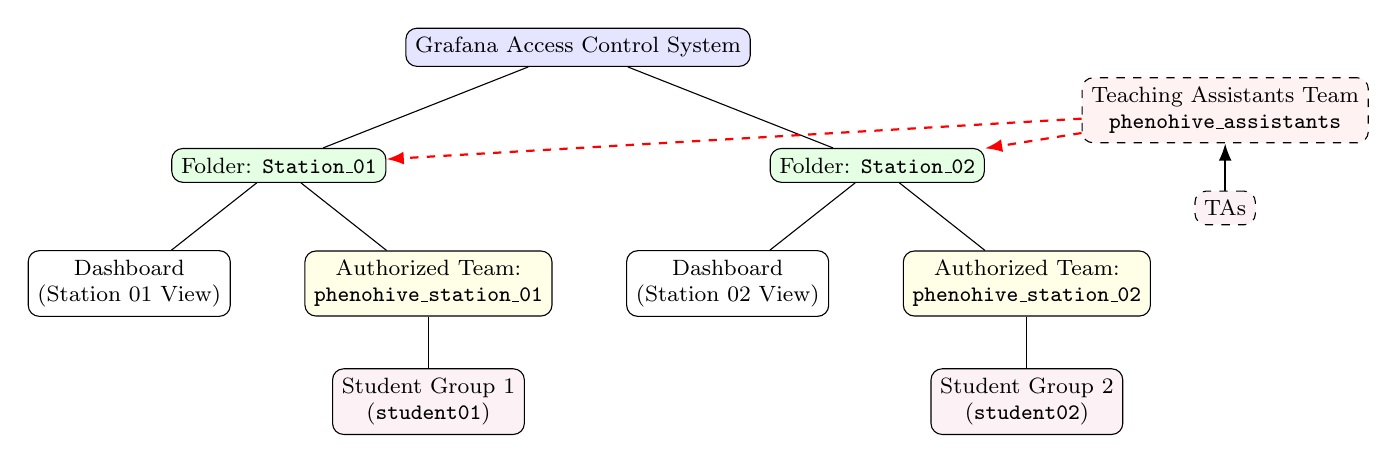
\begin{tikzpicture}[
    level 1/.style={sibling distance=7.6cm, level distance=1.5cm},
    level 2/.style={sibling distance=3.8cm, level distance=1.5cm},
    every node/.style={draw, rounded corners, align=center, font=\footnotesize, fill=white},
    arrow/.style={-{Latex[length=2.2mm]}, thick}
]
\node[fill=blue!10] (root) {Grafana Access Control System}
    child { node[fill=green!10] (f1) {Folder: \texttt{Station\_01}}
        child { node[fill=white] (d1) {Dashboard\\(Station 01 View)} }
        child { node[fill=yellow!10] (t1) {Authorized Team:\\\texttt{phenohive\_station\_01}}
            child { node[fill=purple!5] (u1) {Student Group 1\\(\texttt{student01})} }
        }
    }
    child { node[fill=green!10] (f2) {Folder: \texttt{Station\_02}}
        child { node[fill=white] (d2) {Dashboard\\(Station 02 View)} }
        child { node[fill=yellow!10] (t2) {Authorized Team:\\\texttt{phenohive\_station\_02}}
            child { node[fill=purple!5] (u2) {Student Group 2\\(\texttt{student02})} }
        }
    };

% Global assistants team
\node[draw, dashed, fill=red!5, right=4.2cm of root, yshift=-0.8cm] (assist) {Teaching Assistants Team\\\texttt{phenohive\_assistants}};
\node[draw, dashed, fill=purple!5, below=0.6cm of assist] (uassist) {TAs};

\draw[arrow, dashed, red] (assist) -- (f1);
\draw[arrow, dashed, red] (assist) -- (f2);
\draw[arrow] (uassist) -- (assist);

\end{tikzpicture}
\caption[Grafana Team-Based Permission Topology]{Logical topology of Grafana team-based permission boundaries. Each student group maps to one station folder with one assigned user. The Teaching Assistants team has fleet-wide dashboard access.}
\label{fig:access-control-topology}
\end{figure}

A dedicated Python script called \texttt{sync\_grafana\_access.py} reads these CSV files, calls the Grafana HTTP API, and reconciles the live system to match. It runs every 60 seconds. This allows to add a student to \texttt{users.local.csv} and will lead to the script provisioning the account with an initial password derived from the station ID (intended to be changed by the student on first login), assigning them to their team and finally removing the default viewer rights from every other station folder.

\subsection{Query-level isolation}

A misconfigured or bypassed Grafana permission rule could allow a student to reach another station's dashboard. To prevent any permission bypass from leaking data, a second isolation layer is enforced at the query level.

Every student dashboard is generated as an independent JSON template instance. During the provisioning phase, the auto-provisioning engine clones the master template and hardcodes the station identifier into every Flux query's filter block:
\begin{verbatim}
|> filter(fn: (r) => r.station_id == "01")
\end{verbatim}
Because the dashboard doesn't have any global variables or dynamic dropdown menus allowing students to select different IDs, the browser has no way to request data from other stations. Even if a student inspects the network traffic and captures the raw Flux queries, the credentials associated with their user role restrict them from altering the query parameters on the server preventing any cross-station data access at the query level.

\subsection{Central fleet administration}

While students operate in isolated groups, TAs require a centralized administration panel to be able to oversee the entire station fleet. The \textbf{Grafana Admin Panel} dashboard provides TAs with:
\begin{itemize}
    \item \textbf{Heartbeat indicators}. A color-coded status panel showing ``UP'' or ``DOWN'' for each station. The status is driven by a Flux query that checks whether the station's \texttt{hardware\_uuid} tag has produced any measurement in the preceding 60-minute window:
\begin{verbatim}
from(bucket: "phenohive")
  |> range(start: -1h)
  |> filter(fn: (r) => r._measurement == "phenohive_measurements")
  |> filter(fn: (r) => r.hardware_uuid == "<uuid>")
  |> count()
\end{verbatim}
    A non-zero count maps to ``UP'' (green) while zero or no series maps to ``DOWN'' (red). This one-hour window is a deliberate choice because it tolerates the default 10-minute publish interval plus possible network errors without generating false alerts, while still flagging potetial problematic stations.
    \item \textbf{Raw logging table}. This is just one single unified table that shows the latest records from every active station. Each row contains the station ID, hardware UUID, last-seen timestamp and the last published sensor metrics(temperature, humidity, light and weight). This allows a TA to get a health check on the entire fleet of stationswithout having to open up a single dashboard.
\end{itemize}

The two panels are a deliberately minimal (MVP) admin interface. They are enough for a TA to confirm each station is alive and data is flowing.


\subsection{Data privacy}

The data PhenoHive collects falls under GDPR \parencite{gdprArt6}. It is nothing but environmental sensor readings tagged with a station identifier, with no personal identifiers and no location data. It lives on the UCLouvain VM, is reachable only by the TAs and the group it belongs to and is processed under Article~6(1)(e) for educational research.


\chapter{Deployment and operations}
\label{ch:deployment}

Getting a prototype working is different from getting it deployed at classroom scale. A student with no command-line experience or deep computer knowledge needs to be able to reach a live dashboard within minutes. Also, a TA needs to be able to add a station without needing to interact with the backend. On top of that, twenty stations must push to a shared server without interfering with each other. This chapter describes the deployment architecture that addresses each of these.

\section{Network topology and security architecture}

Each PhenoHive station must push data to the UCLouvain server from wherever a student happens to live, through whatever network is available. The main constraint is that the university VPN requires specific certificates that are difficult to manage in an automated setting. The WireGuard-based overlay and server-side security model described in this section address this.

\subsection{Overlay network rationale}

The UCLouvain VPN \parencite{UCLouvainVPN} isn't designed for devices such as this one because it relies on certificate-based authentication which makes it unsuitable for a fleet of Raspberry Pis that need to be able to connect to it without user interaction. They are also difficult to manage at scale. Another reason is that the University's VPN policy is that it's reserved for university and research staff only. What this means is that even if the technical barriers were overcome, it would not be in accordance with the university's acceptable use policy for students to connect their home devices to the VPN.

To bypass these limitations, this iteration of the PhenoHive project uses Tailscale, a WireGuard-based overlay mesh network \parencite{donenfeld2017wireguard, tailscale}. Tailscale authenticates via pre-provisioned keys, so the Raspberry Pi that runs it has it as a native \texttt{systemd} service called (\texttt{tailscaled}) that reconnects silently on boot without any user interaction. It also uses NAT traversal to go through home routers and establish direct peer-to-peer tunnels (Figure~\ref{fig:network-topology}). While Tailscale is used as the proof-of-concept coordination server due to its ease of setup, the architecture is fully compatible with Headscale which is an open-source, self-hosted alternative for long-term, cost-free production deployment that relies on the same underlying technology \parencite{headscale}.

\begin{figure}[H]
\centering
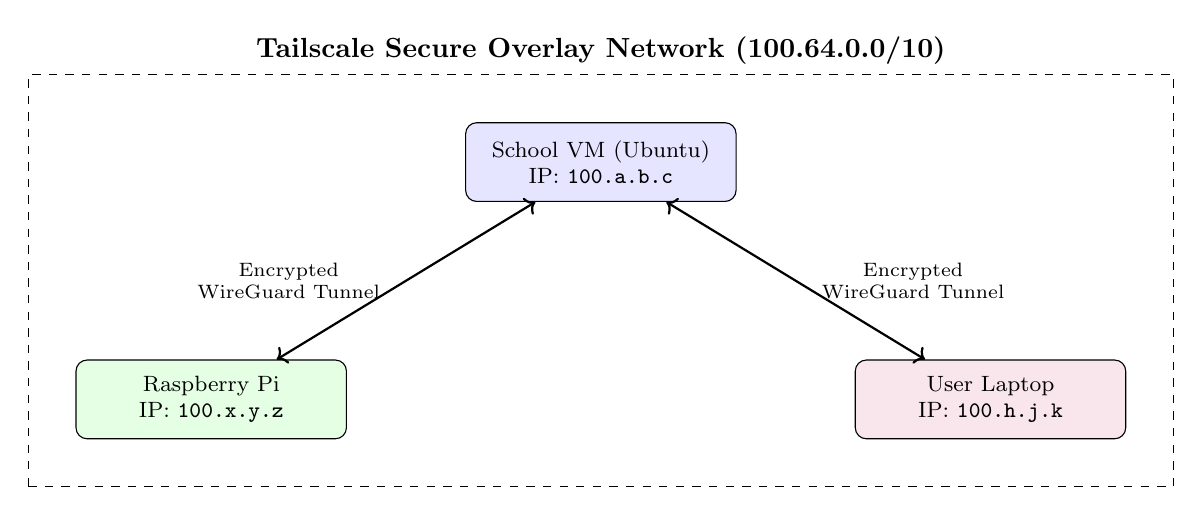
\begin{tikzpicture}[
    node distance=1.2cm and 2.5cm,
    block/.style={draw, rounded corners, align=center, text width=3.2cm, minimum height=1cm, fill=white, font=\footnotesize},
    arrow/.style={<->, thick}
]
\node[block, fill=blue!10] (vm) {School VM (Ubuntu)\\IP: \texttt{100.a.b.c}};
\node[block, fill=green!10, below left=2cm and 1.5cm of vm] (rpi) {Raspberry Pi\\IP: \texttt{100.x.y.z}};
\node[block, fill=purple!10, below right=2cm and 1.5cm of vm] (laptop) {User Laptop\\IP: \texttt{100.h.j.k}};

\draw[arrow] (rpi) -- (vm) node[midway, left, font=\scriptsize, align=center, xshift=-0.2cm] {Encrypted\\WireGuard Tunnel};
\draw[arrow] (laptop) -- (vm) node[midway, right, font=\scriptsize, align=center, xshift=0.2cm] {Encrypted\\WireGuard Tunnel};

\node[draw, dashed, inner sep=0.6cm, fit=(vm) (rpi) (laptop), label={[font=\bfseries]above:Tailscale Secure Overlay Network (100.64.0.0/10)}] (tailscale) {};

\end{tikzpicture}
\caption[PhenoHive Overlay Network Topology]{The PhenoHive overlay network topology. Tailscale establishes a secure WireGuard-based mesh that connects edge devices together with the central VM and user laptops across restrictive networks.}
\label{fig:network-topology}
\end{figure}

\subsection{Virtual machine security and port isolation}

There are three independent layers that protect the central hub VM. First, the UCLouvain firewall filters inbound traffic to the VM's public interface. Then, a host-level UFW ruleset denies by default. And third, Docker port bindings that determine which services are reachable at all.

\paragraph{Public ingress and network-level security}
The UCLouvain's perimeter firewall filters any inbound traffic to the VM's public interface. While port 22 (Secure Shell, SSH) stays open to the internet for remote administration, it's hardened at the OS level and since password authentication is off, this means that only public keys can get in. There is also a \texttt{fail2ban} service that runs at the same time and it blocks any IPs that look like they may be trying to execute a  brute-force attack. The final defense is that operational ports like 3000 (Grafana) and 8081 (Nginx Ingest Proxy) are blocked outright by the university's outer firewall for anything off campus.

In order to not rely solely on the university firewall alone, the VM also runs its own host-level firewall, \texttt{UFW} (Uncomplicated Firewall), set to deny by default. It explicitly permits SSH on the public interface and pushes container traffic through the Tailscale adapter (\texttt{tailscale0}).

\paragraph{Docker network isolation and loopback bindings}
Inside the host OS, Docker's port socket bindings keep each service walled off from one another.

\begin{verbatim}
services:
  influxdb:
    ports:
      - "127.0.0.1:8086:8086" # Bound strictly to VM localhost

  influx_write_proxy:
    ports:
      - "0.0.0.0:8081:8081"   # Open to local interfaces (secured by Tailscale)

  grafana:
    ports:
      - "0.0.0.0:3000:3000"   # Open to local interfaces (secured by Tailscale)
\end{verbatim}

Binding the InfluxDB socket to the loopback interface (\texttt{127.0.0.1}) keeps the database off every external network adapter, the Tailscale overlay interface included. A direct external query to port 8086 is dropped at the host kernel. The only ways in are local sockets, such as administrative CLI commands, or the Nginx write proxy, which runs in a different container on the same host network bridge.

The Nginx write proxy and Grafana are bound to \texttt{0.0.0.0} inside the VM so they can get packets off the overlay. Both of the firewalls still drop public traffic to ports 3000 and 8081 in such a way that only devices that are authenticated on the Tailscale network can reach those interfaces.

\subsection{Edge security and gateway proxy}

By letting a field-deployed device talk straight to the database could create a real risk. If someone physically tampers with a Raspberry Pi, they could pull the database credentials off it and gain full read, write, and delete rights.

In an effort to contain that risk, the Nginx Write Proxy sits on port 8081 and acts as a secure API gateway. It normalises the request formats and only accepts \texttt{POST} requests to \texttt{/api/v2/write} or \texttt{/api/v2/query}. Everything else gets a 403 Forbidden error and is therefore rejected.

\begin{verbatim}
# Nginx write-proxy excerpt (simplified)
location /api/v2/write {
    proxy_pass http://influxdb:8086;
}
location /api/v2/query {
    proxy_pass http://influxdb:8086;
}
location / {
    return 403;
}
\end{verbatim}

So even with a compromised edge token the malicious user can only either append data reads to the \texttt{phenohive} bucket or perform queries. It cannot reach InfluxDB's administrative and management APIs and cannot reconfigure the server. 

\subsection{From sensor to Grafana: the journey of a packet}

Figure~\ref{fig:sensor-to-grafana-path} traces the complete journey of a single packet. Sensor data is formatted into InfluxDB Line Protocol on the RPi, encrypted by WireGuard through the Tailscale overlay, proxied by Nginx into InfluxDB, and finally queried by Grafana for visualization.

\begin{figure}[H]
\centering
\resizebox{\textwidth}{!}{%
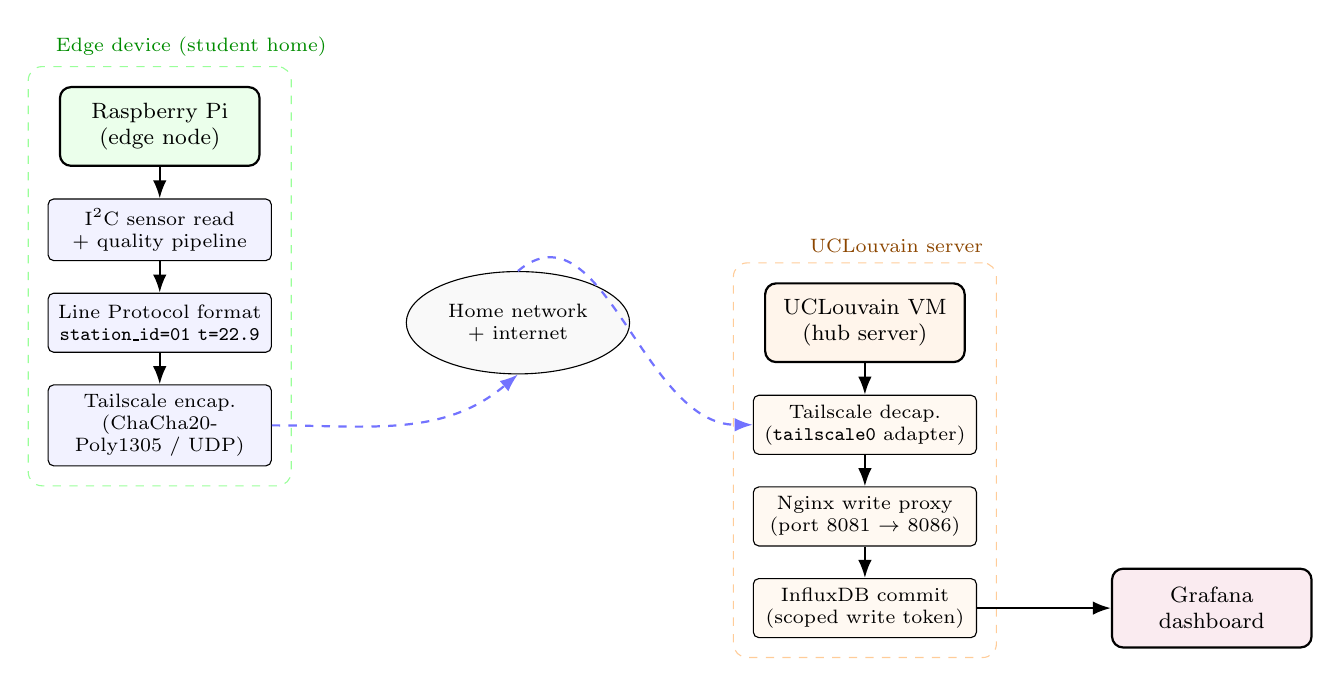
\begin{tikzpicture}[
    node distance=0.45cm and 0.55cm,
    device/.style={draw, thick, rounded corners=4pt, align=center,
        text width=2.3cm, minimum height=1.0cm, font=\footnotesize},
    proc/.style={draw, rounded corners=2pt, align=center,
        text width=2.6cm, minimum height=0.75cm, font=\scriptsize, fill=white},
    arrow/.style={-{Latex[length=2.3mm]}, thick},
    netarrow/.style={-{Latex[length=2.3mm]}, thick, blue!55, dashed}
]

% ---- Edge device ----
\node[device, fill=green!8] (rpi) {Raspberry Pi\\(edge node)};
\node[proc, fill=blue!5, below=0.4cm of rpi] (sense)
    {I$^2$C sensor read\\+ quality pipeline};
\node[proc, fill=blue!5, below=0.4cm of sense] (lp)
    {Line Protocol format\\\texttt{station\_id=01 t=22.9}};
\node[proc, fill=blue!5, below=0.4cm of lp] (tsenc)
    {Tailscale encap.\\(ChaCha20-Poly1305 / UDP)};

\node[draw=green!40, dashed, rounded corners=5pt, inner sep=7pt,
    fit=(rpi)(sense)(lp)(tsenc),
    label={[font=\scriptsize, green!55!black, xshift=0.4cm]above:Edge device (student home)}] {};

% ---- Network cloud ----
\node[draw, ellipse, align=center, font=\scriptsize, fill=gray!5,
    minimum width=2.0cm, minimum height=1.3cm,
    right=1.7cm of lp] (cloud)
    {Home network\\+ internet};

% ---- VM / hub ----
\node[device, fill=orange!8, right=1.7cm of cloud] (vm) {UCLouvain VM\\(hub server)};
\node[proc, fill=orange!5, below=0.4cm of vm] (tsdec)
    {Tailscale decap.\\(\texttt{tailscale0} adapter)};
\node[proc, fill=orange!5, below=0.4cm of tsdec] (nginx)
    {Nginx write proxy\\(port 8081 $\to$ 8086)};
\node[proc, fill=orange!5, below=0.4cm of nginx] (idb)
    {InfluxDB commit\\(scoped write token)};

\node[draw=orange!40, dashed, rounded corners=5pt, inner sep=7pt,
    fit=(vm)(tsdec)(nginx)(idb),
    label={[font=\scriptsize, orange!55!black, xshift=0.4cm]above:UCLouvain server}] {};

% ---- Grafana ----
\node[device, fill=purple!8, right=1.7cm of idb] (grafana)
    {Grafana\\dashboard};

% Edge arrows
\draw[arrow] (rpi) -- (sense);
\draw[arrow] (sense) -- (lp);
\draw[arrow] (lp) -- (tsenc);

% Network traversal
\draw[netarrow] (tsenc.east) to[out=0, in=220] (cloud.south);
\draw[netarrow] (cloud.north) to[out=40, in=180] (tsdec.west);

% VM arrows
\draw[arrow] (vm) -- (tsdec);
\draw[arrow] (tsdec) -- (nginx);
\draw[arrow] (nginx) -- (idb);

% Final arrow to Grafana
\draw[arrow] (idb.east) -- (grafana.west);
\end{tikzpicture}
}
\caption[Secure Data Path from Sensor to Grafana]{The complete path of a single telemetry packet from sensor read to dashboard. The edge device formats data as InfluxDB Line Protocol, encrypts it via Tailscale (WireGuard / ChaCha20-Poly1305), and transmits it over any available internet connection. On the server side, the Nginx write proxy restricts incoming requests to append-only writes before forwarding to InfluxDB, preventing a compromised edge token from reaching administrative endpoints. The grafana dashboard finally queries the database for visualization, completing the data journey.}
\label{fig:sensor-to-grafana-path}
\end{figure}

\section{Station bootstrapping and systemd sequencing}

Each station is identified by a unique \texttt{station\_id} string, set in its local \texttt{config.ini} file. This identifier is attached as a tag to every InfluxDB measurement and establishes the foundation for all downstream data isolation.

\begin{verbatim}
[general]
station_id = 01

[influxdb]
enabled = True
url = http://<SERVER_IP>:8081
token = phenohive-local-dev-token
org = uclouvain
bucket = phenohive
\end{verbatim}

The station identity is deliberately kept minimal: a two-digit string is enough for classroom-scale deployments, and adding a new station requires only flashing the image, setting a unique \texttt{station\_id} and the server ip in \texttt{config.ini}, and starting the service.

To ensure the station boots reliably without any command-line work, the main Python runtime is controlled by a \textbf{systemd service} with a network pre-check (as illustrated in Figure~\ref{fig:boot-chain}). The service unit blocks runtime execution until the network and clock are ready:

\begin{figure}[H]
\centering
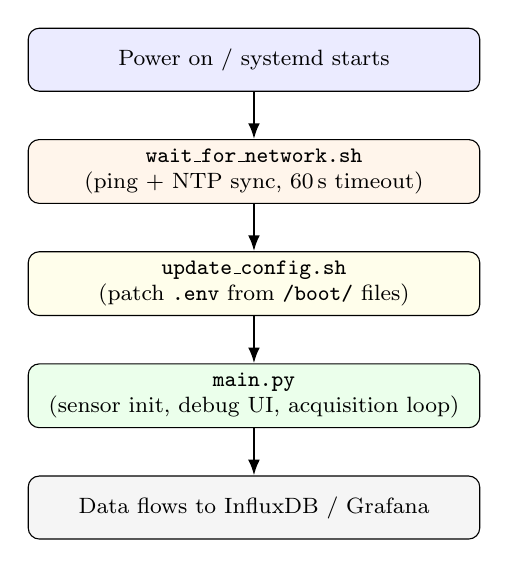
\begin{tikzpicture}[
    node distance=0.6cm,
    block/.style={draw, rounded corners, align=center, text width=5.5cm, minimum height=0.8cm, fill=white, font=\footnotesize},
    arrow/.style={-{Latex[length=2mm]}, thick}
]
\node[block, fill=blue!8] (boot) {Power on / systemd starts};
\node[block, fill=orange!8, below=of boot] (net) {\texttt{wait\_for\_network.sh}\\(ping + NTP sync, 60\,s timeout)};
\node[block, fill=yellow!8, below=of net] (cfg) {\texttt{update\_config.sh}\\(patch \texttt{.env} from \texttt{/boot/} files)};
\node[block, fill=green!8, below=of cfg] (main) {\texttt{main.py}\\(sensor init, debug UI, acquisition loop)};
\node[block, fill=gray!8, below=of main] (data) {Data flows to InfluxDB / Grafana};

\draw[arrow] (boot) -- (net);
\draw[arrow] (net) -- (cfg);
\draw[arrow] (cfg) -- (main);
\draw[arrow] (main) -- (data);
\end{tikzpicture}
\caption[Systemd Boot Chain]{The systemd boot chain from power-on to live data acquisition. Two \texttt{ExecStartPre} directives sequence the pre-start steps. First the network and clock are confirmed as being ready, then the runtime configuration is patched from the boot partition.}
\label{fig:boot-chain}
\end{figure}

\begin{verbatim}
# systemd service pre-start sequencing
[Service]
ExecStartPre=/bin/bash /opt/phenohive/scripts/wait_for_network.sh
ExecStartPre=/bin/bash /opt/phenohive/scripts/update_config.sh
ExecStart=/opt/phenohive/.venv/bin/python main.py
\end{verbatim}

The first pre-start script, \texttt{wait\_for\_network.sh}, executes a loop that blocks service start until an internet connectivity is confirmed via a ping to \texttt{8.8.8.8} and until NTP clock synchronization is completed. This makes sure that all data points carry exact UTC timestamps.

The second and final pre-start script, \texttt{update\_config.sh}, checks the \texttt{/boot} partition for two optional plain-text files: \texttt{phenohive\_server.txt} (containing the hub's IP address) and \texttt{phenohive\_token.txt} (containing the InfluxDB write token). If either file is present, then the script sets the corresponding values into \texttt{/opt/phenohive/.env} before the main runtime starts. Because of the fact that the \texttt{/boot} partition is accessible from any operating system without needing specific mounting tools, a TA can pre-configure a bunch of stations just by writing these files to the SD card from any computer. On first boot, each station is then able to self-configures its server target and token without requiring any SSH access or manual edits to hidden Linux system files.

\section{Auto-provisioning service}

Creating teams, users, dashboards and permissions by hand for each new station is error-prone and time-consuming. The server includes an \textbf{auto-provisioning service} (\texttt{auto\_provision\_grafana.py}) that detects new station identifiers in InfluxDB and provisions the Grafana resources automatically.

The service executes a continuous loop with a 60-second cycle:
\begin{enumerate}
    \item \textbf{Discovery}. It queries InfluxDB using a Flux query to find any and all distinct \texttt{station\_id} tags that are currently present in the database.
    \item \textbf{Provisioning}. For each discovered station ID that does not yet have a corresponding Grafana dashboard associated, the service automatically:
    \begin{itemize}
        \item Creates a new Grafana team (\texttt{phenohive\_station\_XX}).
        \item Creates a student user account called (\texttt{studentXX}) with an initial password that's derived from the station ID.
        \item Clones the master dashboard template and injects the station-specific query filters into it.
        \item Configures folder and dashboard permissions for the new team.
    \end{itemize}
    \item \textbf{Synchronization}. It finally runs the full access-control sync so that any manual changes that the admin made to Grafana are reapplied.
\end{enumerate}

Deploying a new station takes no interaction with Grafana at all. The TA only needs to edit the station's \texttt{config.ini} and starts the service. Within two minutes of the first data push, the auto-provisioning service sees the new station ID in InfluxDB, builds every Grafana resource it needs and the student can then log in.

\subsection{Dynamic station ID reassignment logistics}

In the event of a problem, moving a station from one group to another comes down to a single \texttt{station\_id} change in \texttt{config.ini}. The auto-provisioning service picks up the new ID and builds the new student environment, while the old dashboard keeps its history, and again nobody has to touch Grafana. This can also be done using the debug UI if logged in as admin but it doesn't allow to change the station ID to an existing one.



\chapter{Evaluation and results}
\label{ch:evaluation}

While previous chapters described the design, calibration, and deployment of PhenoHive at the component level, this chapter answers the main question: ``Can a student take a fresh Raspberry Pi, connect it to any Wi-Fi network, and start collecting sensor data on a shared dashboard without opening a terminal?''

\section{Test environment}
\label{sec:test-environment}

Every physical test in this chapter ran on a Raspberry Pi Zero~2\,W with DietPi~9.x, Python~3.11, and the PhenoHive service set up as in Chapter~\ref{ch:deployment}. On the server side, the UCLouvain VM ran InfluxDB~2.7 and Grafana~10.x, reached over the Tailscale overlay. Unless noted otherwise, the station communicated with the server over an ordinary residential Wi-Fi connection.

There are two limitations that apply to all tests. First is that the timing values in Table~\ref{tab:first-boot-timing} come from three to five informal manual observations. This means that they are representative of typical conditions but are not statistically rigorous measurements and that the actual durations may shift with network latency and NTP server response time. The second limitation is that the 20-station concurrent load test (Section~\ref{sec:load-test}) used one physical Raspberry Pi station and 19 software-emulated ones all running as independent Python processes on a development machine. Those emulated stations all share a single Tailscale tunnel and therefore can't reproduce independent residential network variability or hardware-level failures. This means that the test only validates server-side write capacity and auto-provisioning latency. End-to-end residential network behaviour still has to be confirmed in a live deployment.

\section{Deployment and network resilience}
\label{sec:deployment-eval}

\textbf{What was tested.} Headless first-boot onboarding: a student connects a fresh SD card, powers the Pi, and reaches live data on the shared Grafana dashboard with no terminal access.

On first boot, the \texttt{comitup} service creates a temporary hotspot. Opening \href{http://comitup.local}{http://comitup.local} after connecting to it brings up a captive portal (Figure~\ref{fig:comitup-portal}) where the student is able to pick their Wi-Fi network and type in their password \parencite{comitup-service}. The Pi will then reboot and joins the network if the credentials are correct. From there the systemd chain will then initialize the sensors and start pushing data.

\textbf{Result.} The time from power-on to live data on Grafana took under five minutes with no command-line interaction at any point. Table~\ref{tab:first-boot-timing} breaks the timing down by phase.

\begin{figure}[H]
\centering
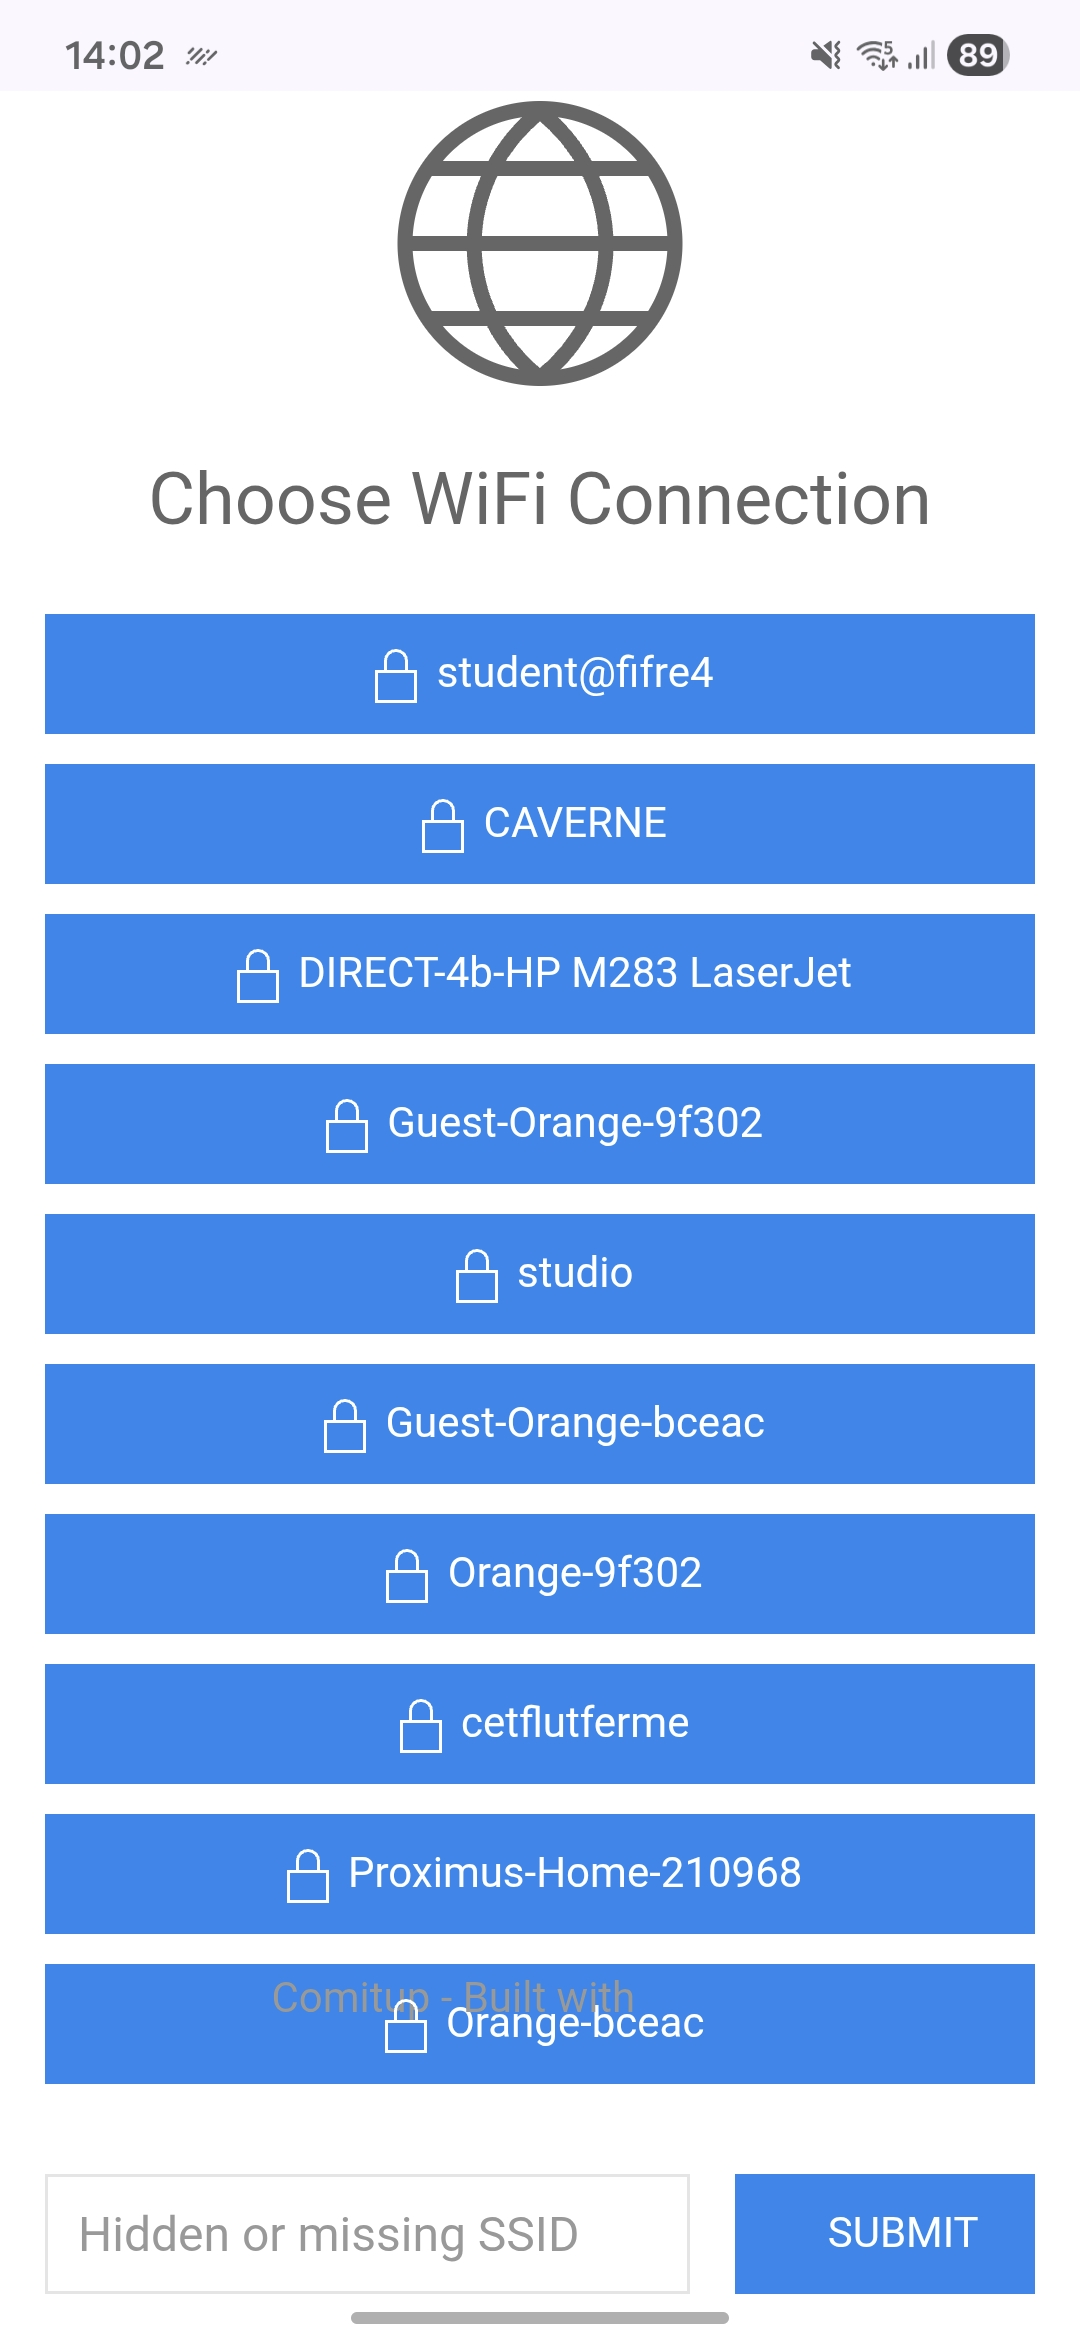
\includegraphics[width=0.4\textwidth]{Images/comitup}
\caption[The Comitup Captive Portal]{The \texttt{comitup} captive portal as seen from a smartphone. The student selects the target Wi-Fi network and enters the password. No SSH or terminal access is required.}
\label{fig:comitup-portal}
\end{figure}

\begin{table}[H]
\centering
\caption[First-Boot Setup Timing Breakdown]{Approximate timing of each phase in the first-boot setup sequence, from power-on to live data visible on the student Grafana dashboard. Values are representative estimates from testing on a Raspberry Pi Zero~2\,W; actual times depend on network speed and NTP server response latency.}
\label{tab:first-boot-timing}
\small
\renewcommand{\arraystretch}{1.25}
\begin{tabularx}{\textwidth}{|P{1.2cm}|P{2.8cm}|X|P{2.2cm}|}
\hline
\textbf{Phase} & \textbf{Milestone} & \textbf{Description} & \textbf{Approx.\ duration} \\
\hline
T0 $\to$ T1 & Power-on & Boot sequence to \texttt{comitup} hotspot broadcast & $\approx$\,45\,s \\
\hline
T1 $\to$ T2 & Portal access & Student connects to hotspot; captive portal loads in browser & $\approx$\,15\,s \\
\hline
T2 $\to$ T3 & Network join & Wi-Fi credentials submitted; Pi reboots and joins target network & $\approx$\,90\,s \\
\hline
T3 $\to$ T4 & Pre-start checks & \texttt{wait\_for\_network.sh}: internet ping and NTP synchronization confirmed & $\approx$\,30\,s \\
\hline
T4 $\to$ T5 & Sensor init & Concurrent \texttt{setup()} calls across all sensors (15\,s global timeout) & $\approx$\,15\,s \\
\hline
T5 $\to$ T6 & First write & First measurement record successfully written to InfluxDB & $\approx$\,10\,s \\
\hline
T6 $\to$ T7 & Provisioning & Auto-provisioning detects new \texttt{station\_id}; Grafana dashboard and student account created & $<$\,60\,s \\
\hline
\textbf{T0 $\to$ T7} & \textbf{Total} & \textbf{Power-on to live data on student dashboard} & $\mathbf{<}$\,\textbf{5\,min} \\
\hline
\end{tabularx}
\end{table}

\section{Runtime behaviour}
\label{sec:runtime-behaviour}

\subsection{Debug UI and on-device calibration}

\textbf{What was tested.} That the on-device web UI gives students access to live sensor readings and guided calibration without any terminal interaction.

The debug UI is a single-page web app that's hosted on port~8080 of the RPI and it has no external dependencies. Its live tab (Figure~\ref{fig:debug-ui-live}) refreshes on its own and shows temperature, humidity, weight and the 14 TCS3448 spectral channel intensities. The calibration tab (Figure~\ref{fig:debug-ui-calibrate}) walks the student through the scale calibration and the camera setup. The admins can also change settings from within this webpage instead of editing the \texttt{config.ini} file directly and see some relevant debugging information.

\textbf{Result.} Every calibration and diagnostics operation ran successfully through the browser, with no command-line interaction needed.

\begin{figure}[H]
\centering
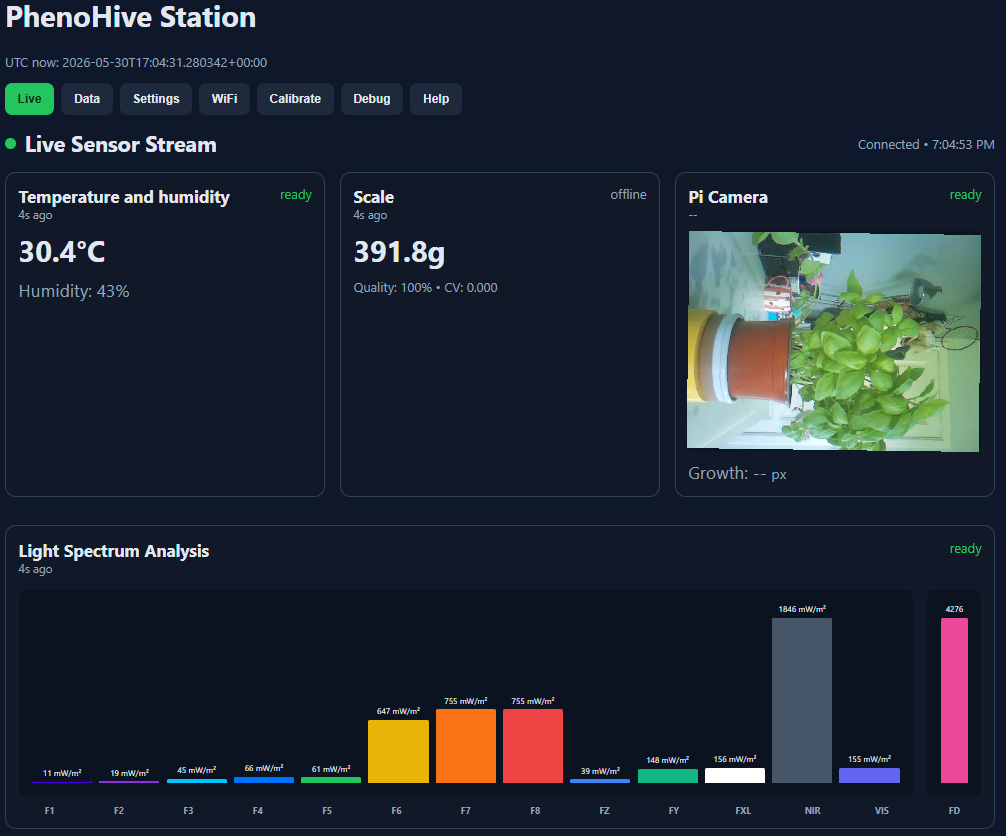
\includegraphics[width=0.85\textwidth]{Images/Debug}
\caption[Debug UI Live Sensor Tab]{The Debug UI live tab showing real-time readings from all sensors. The spectral bar chart (bottom) visualizes the live data from the 14 TCS3448 channels. The temperature, humidity and weight live values are displayed as large numeric cards. The interface refreshes every few seconds via Asynchronous JavaScript and XML (AJAX) polling.}
\label{fig:debug-ui-live}
\end{figure}

\begin{figure}[H]
\centering
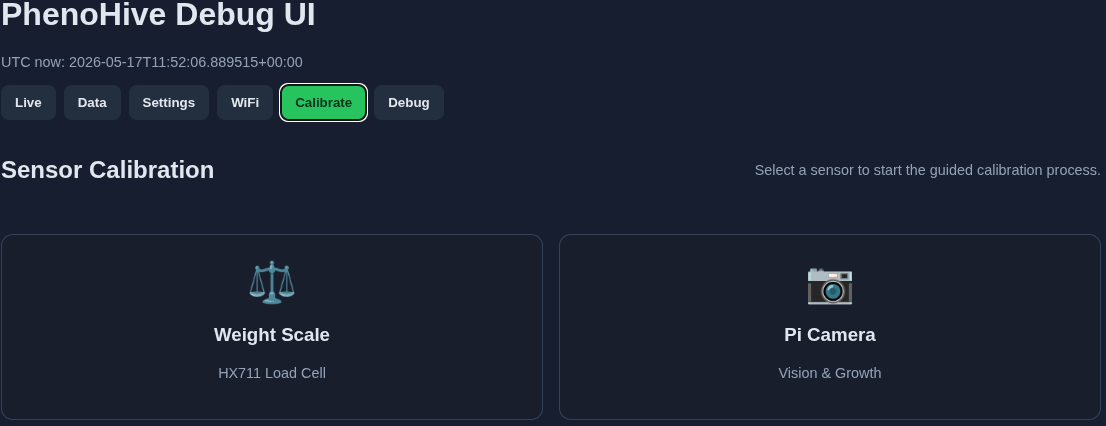
\includegraphics[width=0.85\textwidth]{Images/calibratescreen}
\caption[Debug UI Calibration Wizard]{The guided scale and camera calibration wizards in the Debug UI. Students can calibrate the scale and camera from this easy to understand interface through a guided step-by-step process where no command-line interaction is needed.}
\label{fig:debug-ui-calibrate}
\end{figure}

\subsection{Sensor data quality over a multi-day run}

\textbf{What was tested.} That the full pipeline — burst sampling, MAD outlier filtering, smoothed aggregation, and InfluxDB write — captures continuous, clean environmental data over multiple days.

Figure~\ref{fig:real-sensor-data} shows nine days of data from the physical station (2026-05-18 to 2026-05-27) across three representative channels: air temperature, relative humidity, and TCS3448 spectral channel~F6.

\textbf{Result.} All three channels recorded continuously without any gaps in the data. This demonstrates the long term stability of the platform as a whole.

\begin{figure}[H]
    \centering
    \begin{subfigure}[b]{\textwidth}
        \centering
        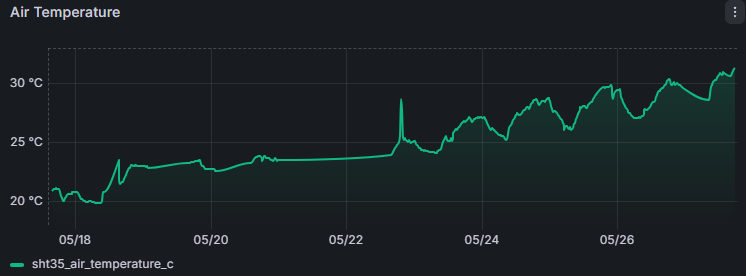
\includegraphics[width=0.92\textwidth]{Images/example_sampling_sht35_temp}
        \caption{Air temperature (\textdegree C), 2026-05-18 to 2026-05-27. A transient spike is visible around 2026-05-22; the two-stage MAD pipeline removes it before the record is persisted.}
        \label{fig:real-data-temp}
    \end{subfigure}
    \vspace{0.5em}
    \begin{subfigure}[b]{\textwidth}
        \centering
        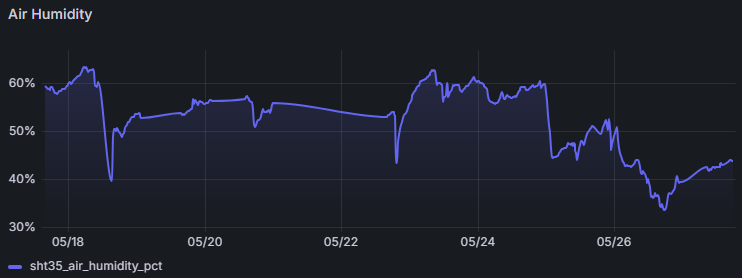
\includegraphics[width=0.92\textwidth]{Images/example_sampling_sht35_hum}
        \caption{Relative humidity (\%\,RH) which was taken during the same period. The trace is clean and continuous with no visible artefacts.}
        \label{fig:real-data-hum}
    \end{subfigure}
    \vspace{0.5em}
    \begin{subfigure}[b]{\textwidth}
        \centering
        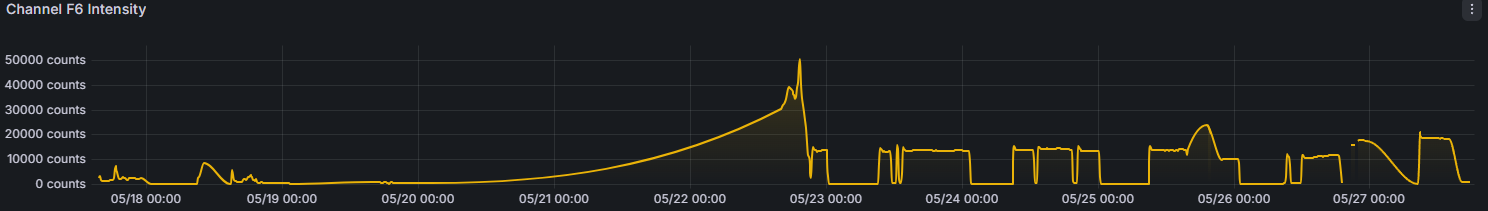
\includegraphics[width=0.92\textwidth]{Images/example_sampling_tcs3448}
        \caption{TCS3448 channel F6 intensity (counts, empirical peak $\sim$600--620\,nm). It shows a clear day and night cycle that reflects the station's lighting environment.}
        \label{fig:real-data-tcs}
    \end{subfigure}
    \caption[Nine Days of Continuous Real Sensor Data]{These are nine days of continuous sensor data from the physical PhenoHive station, as visualized on the Grafana student dashboard. The three channels that are shown here (air temperature, relative humidity, and one TCS3448 spectral channel) demonstrate the pipeline's ability to capture multi-day environmental dynamics with the temporal resolution and data quality required for plant-physiology interpretation. They also show the platform's stability long term.}
    \label{fig:real-sensor-data}
\end{figure}

\subsection{Demonstrative plant observation}
\label{sec:plant-run}

\textbf{What was tested.} That the calibrated sensor suite does indeed detect the physiological signals that the course targets when monitoring an actual potted plant. These are cumulative water loss via the pot-mass channel, atmospheric evaporative demand derived from the calibrated temperature and humidity, and light-cycle structure from the spectral channel.

A potted plant was placed on the station and monitored from 2026-05-29 to 2026-05-31 without watering. This allowed an uninterrupted trace across all channels to be made (Figure~\ref{fig:plant-run}).

The plant mass (Figure~\ref{fig:plant-run-mass}) declined linearly from 478\,g to 353\,g over 54 hours which represents a total loss of 125\,g or ($\approx$55\,g/day). Two features of this trace are notable. First is that the decline is nearly linear with no day-night acceleration. This strongly suggests that a load-cell drift under sustained load is contributing to a constant offset alongside the real water loss. The HX711 ADC is known to drift with temperature changes over hours-to-days timescales. The calibration that was carried over from \textcite{colinet2025} provides no drift correction. Second, slope changes over shorter windows (1--2 hours) remain qualitatively interpretable. A periodic re-taring protocol which is identified as future work in Section~\ref{sec:future-work} would restore quantitative multi-day accuracy.

Temperature (Figure~\ref{fig:plant-run-temp}) however remained in the 29.5--31\,°C range with a $\approx$1\,°C diurnal amplitude. This is warmer than typical indoor conditions but was due to the weather conditions at the time of recording. Relative humidity (Figure~\ref{fig:plant-run-hum}) also rose from $\sim$42\,\%\,RH to 45--46\,\%\,RH over the test cycle with a step increase overnight on May~30th and 31st which is consistent with the plant humidifying the air that surrounds the sensor. 

The TCS3448 F4 channel (Figure~\ref{fig:plant-run-tcs3448} empirical peak $\sim$480--500\,nm, cyan-green) shows a clear natural day-night light cycle. The intensity rises from near zero at night to about 600--730\,mW/m$^2$ during the afternoon. The day-to-day variation in peak intensity reflects the changing outdoor illumination instead of just some sensor artefact.

\textbf{Result.} The temperature, humidity and spectral channels functioned continuously and captured the expected physiological structure. The mass channel however revealed a drift artefact that limits absolute multi-day rate comparisons but does not affect short-term trend analysis. This is due to a calibration-maintenance issue, not an architectural one. Together the four channels demonstrate that the platform manages to capture the signals that the course requires and that the calibrated environmental data can already fully support the stomatal-response reasoning that the course expects.

\begin{figure}[H]
    \centering
    \begin{subfigure}[b]{\textwidth}
        \centering
        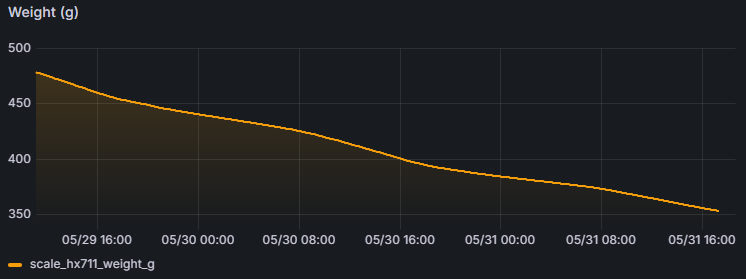
\includegraphics[width=0.92\textwidth]{Images/hx711_plant_test}
        \caption{Pot mass (g), 2026-05-29 to 2026-05-31. The nearly linear decline from 478\,g to 353\,g over about 54\,h ($\approx$55\,g/day) combines real evapotranspiration and load-cell drift. But due to the absence of day/night rate variation, it confirms that sensor drift dominates.}
        \label{fig:plant-run-mass}
    \end{subfigure}
    \vspace{0.5em}
    \begin{subfigure}[b]{\textwidth}
        \centering
        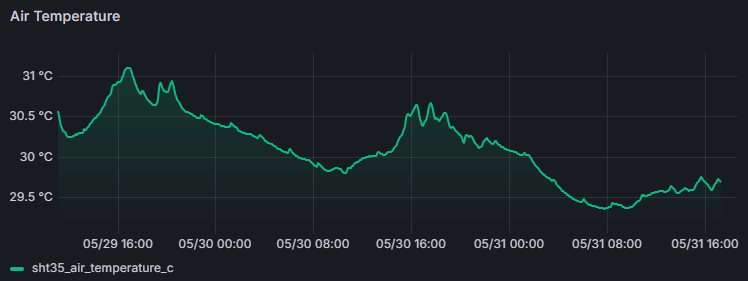
\includegraphics[width=0.92\textwidth]{Images/sht35_temp_plant}
        \caption{Air temperature (\textdegree C) during the same period. Warm and stable (29.5--31\,°C) with $\approx$1\,°C diurnal amplitude.}
        \label{fig:plant-run-temp}
    \end{subfigure}
    \vspace{0.5em}
    \begin{subfigure}[b]{\textwidth}
        \centering
        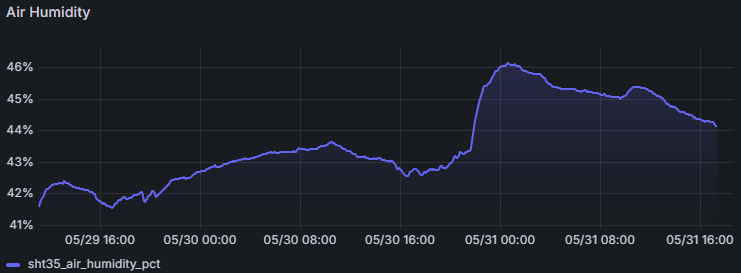
\includegraphics[width=0.92\textwidth]{Images/sht35_hum_plant}
        \caption{Relative humidity (\%\,RH) with again the same period. The rise from $\sim$42\,\% to 45--46\,\% is consistent with the plant humidifying the nearby air.}
        \label{fig:plant-run-hum}
    \end{subfigure}
    \vspace{0.5em}
    \begin{subfigure}[b]{\textwidth}
        \centering
        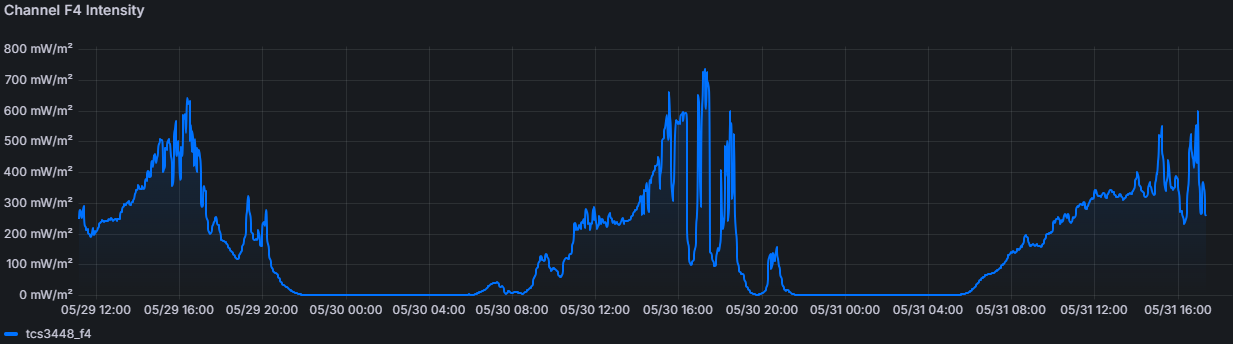
\includegraphics[width=0.92\textwidth]{Images/tcs3448_plant_test.jpg}
        \caption{TCS3448 channel~F4 (mW/m$^2$, with an empirical peak at $\sim$480--500\,nm). Natural day and night cycles are clearly visible. With a near zero value at night and 600--730\,mW/m$^2$ at afternoon peak. The day-to-day variation in peak intensity reflects changing outdoor illumination.}
        \label{fig:plant-run-tcs3448}
    \end{subfigure}
    \caption[54-Hour Plant Observation]{54-hour demonstrative plant observation (2026-05-29 to 2026-05-31).}
    \label{fig:plant-run}
\end{figure}

\subsection{Multi-station isolation and dynamic provisioning}

\textbf{What was tested.} That data is isolated per student and that reassigning a station ID triggers correct re-provisioning without data loss.

Running a physical Station~01 at the same time as a Docker-based mock Station~02 confirmed isolation at both the query and permission levels. Each student login returned only its own station's data as expected(Figures~\ref{fig:grafana-admin}--\ref{fig:grafana-student}).

To test out the dynamic provisioning path, Station~01's ID was changed to \texttt{04} through the debug UI.

\textbf{Result.} The auto-sync service built the new Grafana environment (dashboard and user account) in about two minutes. The original Station~01 dashboard retained its full history but stopped receiving new data once the ID was changed. No data loss occurred during the transition.

\begin{figure}[H]
\centering
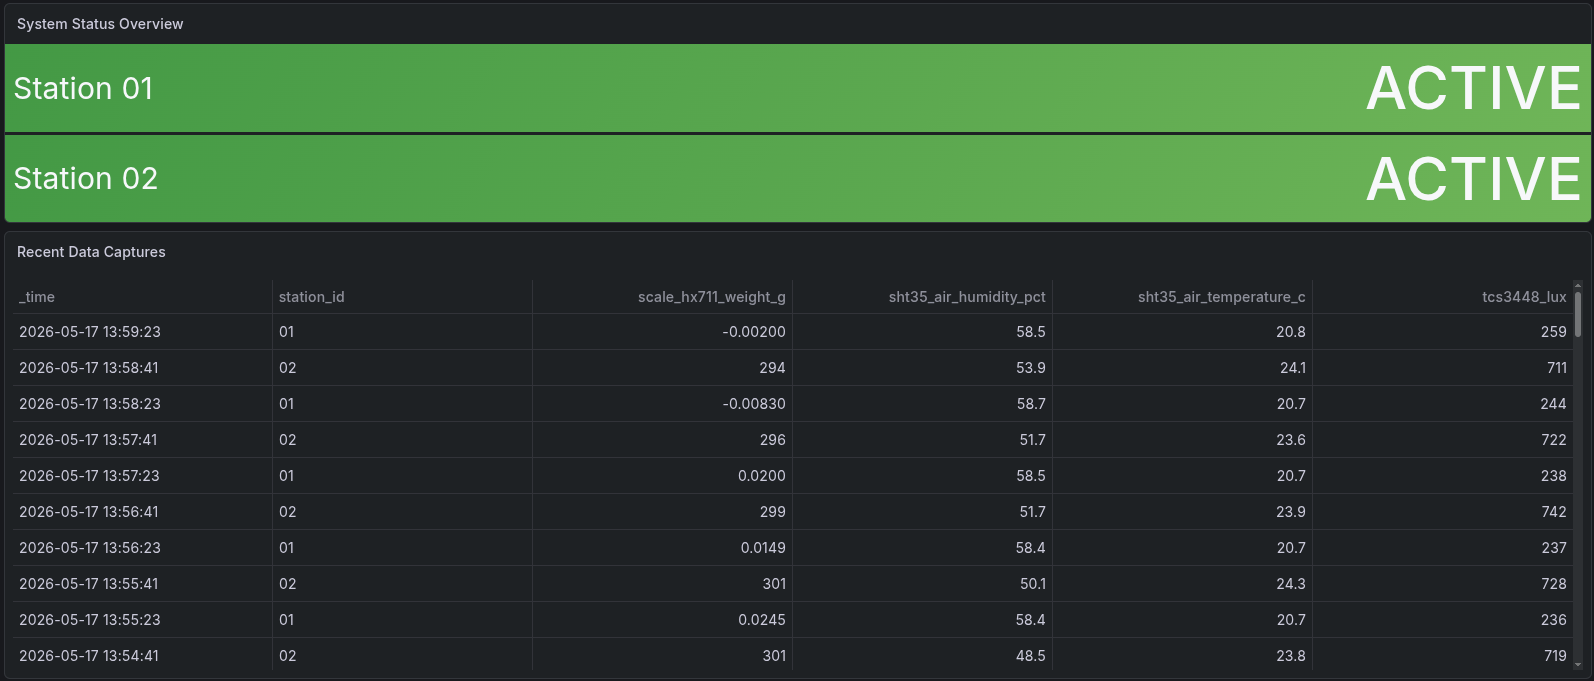
\includegraphics[width=0.85\textwidth]{Images/admingrafana}
\caption[Grafana Admin Panel]{The Grafana Admin Panel showing two active stations. Station~01 runs on physical hardware and Station~02 is a Docker-based mock. Both report the ``UP'' status with their most recent measurements visible in the unified table.}
\label{fig:grafana-admin}
\end{figure}

\begin{figure}[H]
\centering
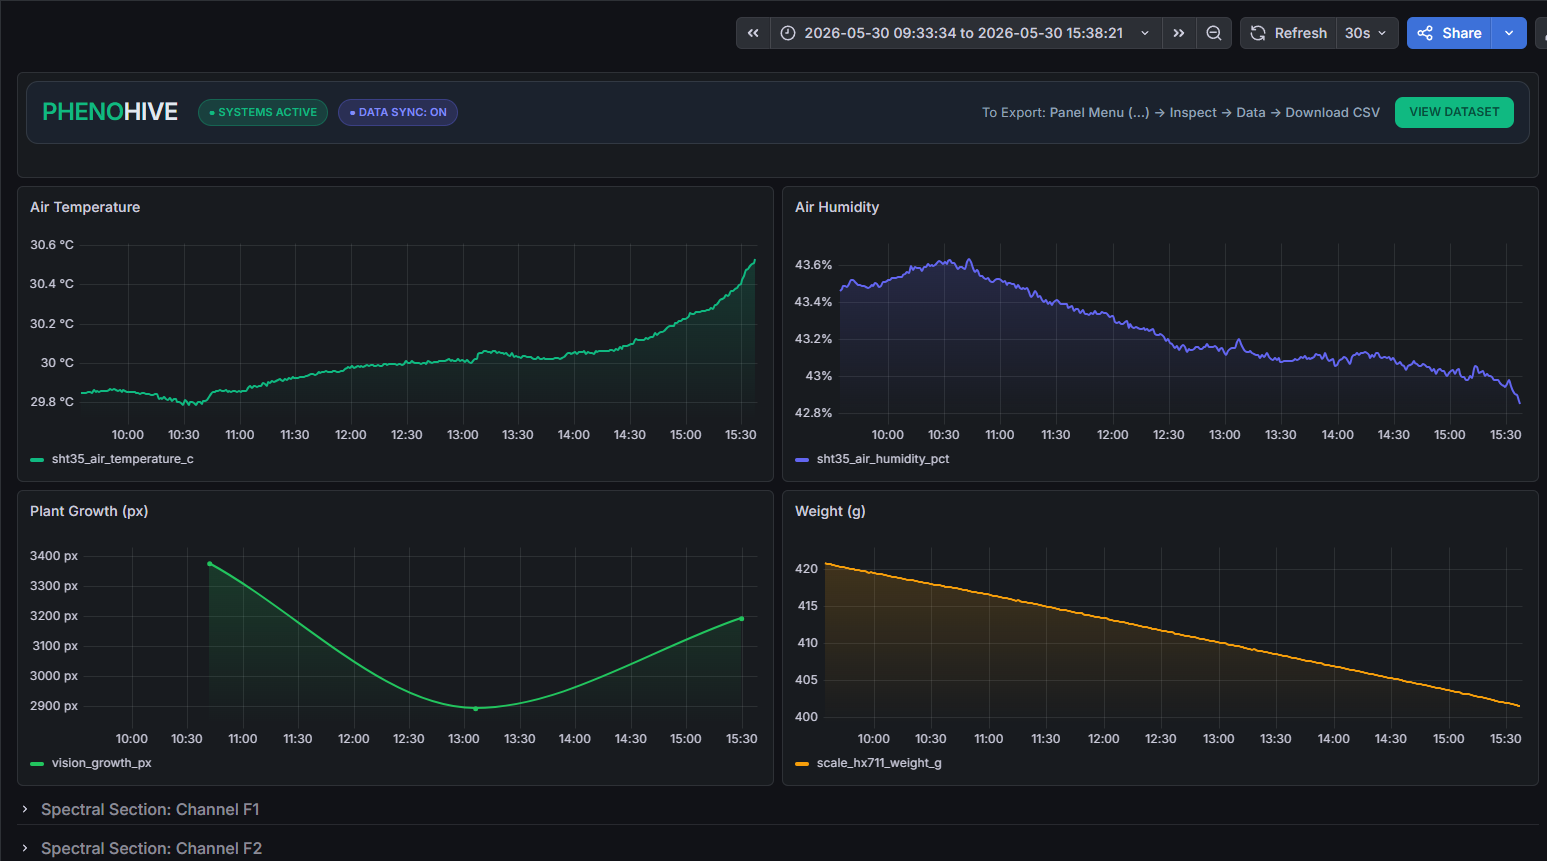
\includegraphics[width=0.85\textwidth]{Images/studentdashboard}
\caption[Student-Facing Grafana Dashboard]{The student-facing Grafana dashboard for Station~01 which shows the time-series panels for temperature, humidity, spectral irradiance and plant weight. Logging in as \texttt{student02} would displays an identical layout but with only Station~02 data, as explained to establish query-level isolation.}
\label{fig:grafana-student}
\end{figure}

\subsection{Concurrent load test}
\label{sec:load-test}

\textbf{What was tested.} Server-side write capacity and auto-provisioning latency with 20 stations writing concurrently (1~physical + 19~software-emulated).

The 19 emulated stations all ran as independent Python processes on a development machine. They were all writing through to the same Nginx proxy to the shared InfluxDB instance. The run lasted a total of 3 hours at an accelerated 30\,s/60\,s collection and publish rate to simulate real-world usage.

\textbf{Result.} Not a single station produced an offline queue file. The auto-provisioning service had all 19 dashboards up within 60--90\,s of each station's first write which confirms that the server-side write capacity and that the provisioning latency hold up at classroom level scale. As noted in Section~\ref{sec:test-environment}, the emulated stations shared a single Tailscale tunnel and could not reproduce independent residential network variability. This means that the end-to-end home-network behaviour still needs validation in a live deployment.

\section{Validation summary}
\label{sec:eval-summary}

Table~\ref{tab:eval-summary} lists all validation scenarios and their outcomes, with traceability to the original requirements.

\small
\renewcommand{\arraystretch}{1.3}
\begin{longtable}{|P{3.0cm}|p{\dimexpr\textwidth-3.0cm-2.5cm-1.8cm-8\tabcolsep-5\arrayrulewidth\relax}|P{2.5cm}|P{1.8cm}|}
\caption[System-Level Validation Test Summary]{Summary of system-level validation tests and their traceability to the original requirements. All tests were performed on physical hardware (Raspberry Pi Zero 2~W) except the 20-station load test (1 physical + 19 software-emulated).}
\label{tab:eval-summary} \\
\hline
\textbf{Test scenario} & \textbf{Expected outcome} & \textbf{Outcome} & \textbf{Req.} \\
\hline
\endfirsthead
\multicolumn{4}{l}{\small\itshape (Table~\ref{tab:eval-summary} continued from previous page)} \\[2pt]
\hline
\textbf{Test scenario} & \textbf{Expected outcome} & \textbf{Outcome} & \textbf{Req.} \\
\hline
\endhead
\hline
\endlastfoot
Headless Wi-Fi setup (fresh SD card) & Station broadcasts hotspot, accepts credentials via captive portal, begins data acquisition & Pass ($\sim$5\,min first-boot) & R3, R4 \\
\hline
Network relocation (new Wi-Fi) & Falls back to hotspot, accepts new credentials, resumes without data loss & Pass & R3 \\
\hline
48-hour server disconnection & All measurements buffered locally and replayed in order upon reconnection & Pass (no data loss observed) & R3 \\
\hline
Power-cycle reboot & Automatic reconnection and uninterrupted data resumption & Pass & R3 \\
\hline
Calibration persistence across code updates & Scale tare and factor survive deployment script execution & Pass & R3, R5 \\
\hline
Camera concurrency & Sensor polling continues at 10\,s collection interval during image capture (interval reduced from 120\,s for test visibility) & Pass & R3 \\
\hline
Sensor failure recovery & Acquisition loop continues for other sensors, and failed sensor data resumes automatically upon reconnection & Pass & R3 \\
\hline
I$^2$C bus recovery under service restart & TCS3448 and SHT35 initialize correctly after a service restart that follows an ungraceful process termination; the in-process recovery mechanism (\texttt{SensorFactory.\_run\_i2c\_recovery()}) clears the stuck bus state before each sensor setup retry & Pass & R3 \\
\hline
Persistent sensor failure watchdog & SHT35 or TCS3448 remaining in \texttt{ERROR} state for 30~min triggers an automatic service restart; both sensors recover within the first retry cycle of the new process & Pass (recovered in 1 retry cycle) & R3 \\
\hline
Station ID conflict detection & Attempting to claim an ID owned by another device is rejected & Pass & R6 \\
\hline
Multi-station data isolation & Each student login sees only their station's data & Pass & R6 \\
\hline
Dynamic ID reassignment & New Grafana environment created within 2 minutes, old dashboard retains history & Pass ($<$2\,min provisioning) & R5, R6 \\
\hline
20-station concurrent load (1 physical + 19 mock) & All write requests acknowledged, no offline queue files, all 19 dashboards auto-provisioned within 90\,s & Pass (0 queued, 19 dashboards in $<$90\,s) & R3, R6 \\
\hline
\end{longtable}
\normalsize

The validation campaign confirmed that the current implementation meets all six original requirements. Headless onboarding, multi-day network resilience, sensor-failure recovery, multi-station isolation, and concurrent 20-station operation were each demonstrated on physical hardware or a close emulation. The result that matters most in practice is the five-minute first boot: a fresh station with no prior configuration reaches live data on the shared dashboard with no command-line interaction, which is exactly the usability bar a teaching platform has to clear.

\chapter{Discussion}
\label{ch:discussion}

\begingroup
\setlength{\parskip}{0.6em}

This objective of this chapter is to examine the implementation against its stated objectives, identifies what holds up under scrutiny, where the gaps remain, and what aspects require more attention.

\section{Revisiting the thesis' original objectives}

All three original objectives were met. The architecture became much clearer once the code was rewritten into four bounded source packages behind a factory-based sensor abstraction. Sensing quality came from the WELCOME-lab calibrations, which corrected a roughly 25\,nm TCS3448 channel shift and brought down environmental factor uncertainty down. And deployment resilience held up on real hardware, the station handles out 48-hour disconnections without losing data and reaches live Grafana data in under five minutes from first boot.

\section{Limits of the current implementation}

\subsection{Calibration validity and reproducibility}

The environmental and spectral calibrations were only performed once on a single station at the WELCOME lab. For a platform that will eventually include around 20 units, that creates a few problems.

The TCS3448's spectral response is not perfectly uniform across all manufacturing batches. This means that the roughly 25\,nm empirical shift that's documented in Chapter~\ref{ch:data-acquisition} could differ between individual sensors, but the current calibration applies the same per-channel scale factors to every unit. For rigorous spectral comparisons across student groups, each sensor would need its own monochromator sweep.

The SHT35 calibration also only relied ona single reference which means that it carries the same risk. The factory calibration is very good. Still, the 0.1--0.3\,°C offset seen during validation hints that some units may drift further than others. A batch calibration against a high-precision reference like the one used in the WELCOME lab would ideally confirm that every station are within an acceptable margin.

\subsection{Scale and multi-station validation}

The initial evaluation ran with two stations. One physical station with real hardware and one Docker-based mock. The classroom-scale load test in Section~\ref{sec:load-test} pushed that to the full targeted number by using one physical plus 19 mock stations. The write proxy, InfluxDB, and the auto-provisioning service all were able to handle the 20 concurrent stations pushing data with no data loss and no provisioning failures.

Two questions however still remain open. The first is how the auto-provisioning service performs under sustained load, which fires on the order of 100 Grafana API calls per 60-second sync cycle at full cohort size. The second is cardinality over longer horizons: 14 spectral channels per station at a 10-minute publish interval add up to roughly $20 \times 6 \times 24 \times 30 = 86\,400$ data points per channel per month across the cohort (stations × writes/hour × hours/day × days/month). The 60\,s publish rate in the load test stood in for heavier write pressure than the default 600\,s, and nothing went wrong during the test window, but a full month of real data from 20 stations has not been benchmarked at production intervals.

\subsection{Networking and connectivity assumptions}

The station currently relies on the Tailscale VPN to reach the central server through restrictive networks. Tailscale is a commercial service, so if it goes down, stations stay offline until it recovers. The offline replay queue keeps the data safe, but students would lose live dashboard updates during such an outage. For a large deployment, like the one this thesis aims to support, cost is a factor too. The self-hosted alternative, Headscale, settles both concerns, but requires an infrastructure configuration to be able to run it.

\subsection{Camera pipeline}

The vision pipeline is inherited from \textcite{colinet2025} and was not re-evaluated here. A threading fix resolved the blocking regression introduced by the single-threaded capture design, but the PlantCV segmentation and its accuracy under varied indoor lighting was not re-tested.

\section{Pedagogical fitness}

The central pedagogical question (whether a student in the LBIR1251 course can take the numbers from their dashboard and use them to reason about stomatal conductance, phytochrome signalling, or water balance) is not answered by this thesis. PhenoHive has not yet been deployed in a real LBIR1251 class, and no student learning outcomes have been measured. 

The sensor suite meets the preconditions that are necessary for the type of analysis conducted in the LBIR1251 course, but whether students can reliably translate the data into correct physiological conclusions is an open empirical question.

\paragraph{What remains a hypothesis (to be tested).}
Three things stay hypothetical. First is whether students can read this data and draw correct physiological conclusions. Second is whether the better data quality changes how they design experiments. And third is whether the lower hardware friction buys them more time on analysis instead of troubleshooting. Settling them needs a structured evaluation with real student groups, ideally comparing the quality of experimental analysis between groups. This as the single most important next step.

\section{Future work}
\label{sec:future-work}

\paragraph{Per-station spectral calibration.}
Calibrating the TCS3448 sensor against the monochromator took about two hours including the time it took to setup. Automating that sweep with the DOPES library \parencite{dopes}, which already provides a Python interface for the CM110 and power meter, and writing a script to compute the per channel offsets from the resulting dataset would greatly reduce the calibration time. Each station would then be able to carry its own characterization instead of sharing a single one, making the spectral comparisons across student groups even more defensible and precise.

\paragraph{Automated calibration drift monitoring.}
A lightweight software check on the scale baseline could flag when the resting mass drifts more than what normal plant growth or evaporation would explain. This would allow the TA to see a warning before the student even notices the readings are off.

\paragraph{Migration to Headscale.}
Swapping out the Tailscale platform for a self-hosted Headscale instance on the UCLouvain servers allows for removing the commercial dependency without touching the station firmware. This would be a one-time infrastructure job that would make the platform considerably more self-reliant and secure.

\paragraph{Soil moisture and temperature sensing.}
Soil moisture and temperature were dropped from this thesis for time and scope reasons, even though these metrics both feed straight into the course's material. Adding a sensor of that class through the existing factory pattern is very manageable. The real work would rely in calibrating it and presenting the data at the right level for the class.

\paragraph{CO\textsubscript{2} monitoring.}
A CO\textsubscript{2} sensor would provide a direct view of net photosynthetic activity that no current channel gives. The main factor that keeps it from being added is cost as a calibrated Non-Dispersive Infrared (NDIR) sensor that stays reliable in an uncontrolled environment costs more than any of the I$^2$C sensors already in the suite.

\paragraph{Month-long evaluation.}\label{sec:future-work-month}
PhenoHive has yet to run through an actual LBIR1251 class. A structured evaluation, measuring student engagement, report quality and conceptual understanding against a comparison group on the traditional protocols, would supply the evidence needed to judge whether the platform really changes and improves how students learn. That study should follow the first real deployment.

\section{Reflection on the development process}

Working on the third generation meant deciding which open problems were worth the remaining effort. The earlier theses had already proved that the hardware was feasible and that the data is useful. The main danger this time was scope creep, adding more and more features onto a codebase that was already hard to maintain would've been problematic.

Refactoring first paid off in a concrete way when the monochromator sweep turned up the channel-mapping error in the TCS3448, the fix was pretty easy as it only required a simple configuration-file edit, because the sensor abstraction was already clean. The 48-hour disconnection test was a similar story. The local-first persistence model behaved exactly as designed, and the buffered records flushed cleanly once the network connectivity returned. Both outcomes confirmed that the choices that were made were the right ones.

One configuration fault ended up proving that point as well. The InfluxDB write URL was mistakenly pointing at the station's loopback address instead of the VM's Tailscale address. This opened up a one-hour data gap. The offline queue caught every record during that time. After fixing the URL over SSH, the system restored the write path at once and the local archive had worked as a real safety net under an actual configuration error because all the data that was gathered during the outage was pushed at the very next cycle.

Altogether, the development process was a good example of how to balance refactoring and feature development, and how to design for failure in a way that makes the system resilient to the inevitable mistakes and oversights that happen during development.
\endgroup


\chapter{Conclusion}
\label{ch:conclusion}

\begingroup
\setlength{\parskip}{0.6em}

The approach this thesis took was not a rebuild from scratch, but more a careful look at what the platform was actually doing, and an effort to improve or correct what was not working. The work was organized around three objectives. These were defined as architectural clarity, sensing quality, and deployment resilience. The previous iterations had established what the concept is and the hardware choices are. What was left to do was consolidating them into a platform that could be trusted in uncontrolled environments by students who should not need to think about the measurement system and the quality of the data. Two components are explicitly carried over from the previous theses and weren't reevaluated here. These are the PlantCV vision pipeline and HX711 mass-channel calibration from \textcite{colinet2025} and the DietPi deployment model from \textcite{goffinet2024}.

\section*{Original contributions}
\addcontentsline{toc}{section}{Original contributions}

The three objectives decompose into eight specific contributions, each of which was absent from both preceding PhenoHive theses:

\begin{enumerate}
    \item \textbf{Modular software architecture.} Refactoring the codebase from a simple monolithic script into an easily maintainable codebase with four Python source packages (\texttt{core}, \texttt{sensors}, \texttt{ui}, and \texttt{vision}) under \texttt{src/}, with a \texttt{scripts/} directory of operational helpers, and a factory-based sensor abstraction (\texttt{BaseSensor}) that allows for new hardware to be added without needing to modify the acquisition loop.

    \item \textbf{SHT35 metrological calibration.} A four-point corner sweep against the WELCOME lab's Espec SH-242 climatic chamber, which produced traceable linear corrections ($+0.14\,^\circ$C, $-1.53\,\%$\,RH) which were applied to every reading in the platform, allowing the student to trust the numbers and recieve precise measurements that will allow them to reason more carefully about the environmental conditions.

    \item \textbf{TCS3448 spectral calibration and channel mapping.} A full 300--940\,nm monochromator sweep with two diffraction gratings, which exposed a systematic shift of roughly 25\,nm across the visible channels and fixed per-channel dark offsets and irradiance scale factors (counts to mW/m$^2$). The empirical mapping it produced replaces the nominal values that were provided by the datasheet everywhere in the platform. This means the student can now read the spectral data in physical units, and reason about the light environment in terms of photosynthetically active radiation instead of raw counts. It means they can also trust the readings provided by the platform and be able to more easily figure out what affects their plant's growth.

    \item \textbf{Local-first persistence with offline replay.} A CSV-first append model keeps the authoritative archive independent of network availability. So it being paired with a JSONL offline queue that buffers records and replays them to InfluxDB on reconnection is a robust solution. A deliberate 48-hour disconnection test confirmed it. Students can therefore truly trust that their data is being recorded even when the network drops and that it will still be there when they come back.

    \item \textbf{Headless Wi-Fi onboarding.} Integration of the Comitup captive-portal service which lets a student set up the network on first boot with no command line at all. It allows for power-on to live data on Grafana that was measured in at under five minutes. A student gets the station online and running without needing to ask for help or to know anything about system configuration.

    \item \textbf{Tailscale overlay network and Nginx write proxy.} An encrypted peer-to-peer VPN in place of the certificate model, together with a restrictive write-only proxy that stops a compromised edge token from ever reaching InfluxDB's administrative endpoints. This secures the network without needing to manage certificates, and allows the station to be deployed on any network that allows outbound VPN connections, without needing to ask for permission or have prior knowledge in networking.

    \item \textbf{Auto-provisioning service.} Continuous InfluxDB polling that picks up new \texttt{station\_id} values and builds isolated Grafana teams, dashboards, and student accounts on its own, cutting per-station setup to zero Grafana interaction. Adding a station to the deployment no longer means working through tedious configuration tasks.

    \item \textbf{Two-stage MAD signal-processing pipeline.} Burst-level and cross-collection Median Absolute Deviation filtering, with explicit quality metadata (\texttt{low\_confidence}, coefficient of variation, success ratio) attached to every published record. This means that the student can filter out bad data with confidence, and that they can understand why a particular reading is flagged as low-confidence.
\end{enumerate}

On physical hardware, the evaluation chapter answered the engineering half of the research question. A student can take a freshly-imaged Raspberry Pi, bring it online through the Comitup captive portal, and reach calibrated multi-sensor data on a private Grafana dashboard in under five minutes, never touching a command line. The pedagogical half is the part this thesis cannot answer yet. Whether students will really be able to use the data to reason more carefully about stomatal conductance, phytochrome signalling or water balance. Only a real deployment will reveal the answer, and the platform is now in a state where that's possible. The sensor suite is metrologically validated, the network holds up, provisioning is fully automated, and the station recovers from the disconnections and surprise reboots that are routine in a home. Together, these move PhenoHive from a prototype to a fully fledged system that can be deployed. 


\endgroup



% ── Appendices ─────────────────────────────────────────────────────────────────
\appendix
\chapter{Technical architecture}
\label{ch:appendix-technical}

\section{Electronic wiring diagram}
\label{sec:appendix-wiring}

Figure~\ref{fig:wiring-schematic} provides the complete electronic wiring schematic for assembly and troubleshooting reference.

The station is centered around a Raspberry Pi Zero 2~W \parencite{rpi-zero-2w}. Three bus distribution headers consolidate the 3.3\,V, 5\,V, and Ground rails to reduce wire congestion. The environmental (SHT35) and multi-spectral (TCS3448) sensors both share a single I$^2$C bus communicating over General Purpose Input/Output (GPIO) 2 (SDA) and GPIO 3 (SCL). The HX711 24-bit analog-to-digital converter is connected via a digital interface over GPIO 5 (DOUT) and GPIO 6 (SCK). The KY-019 relay module controlling the 5\,V COB LED strip is connected to GPIO 23 (BCM). The camera module is connected via a CSI interface directly to the Raspberry Pi.

\begin{figure}[H]
\centering
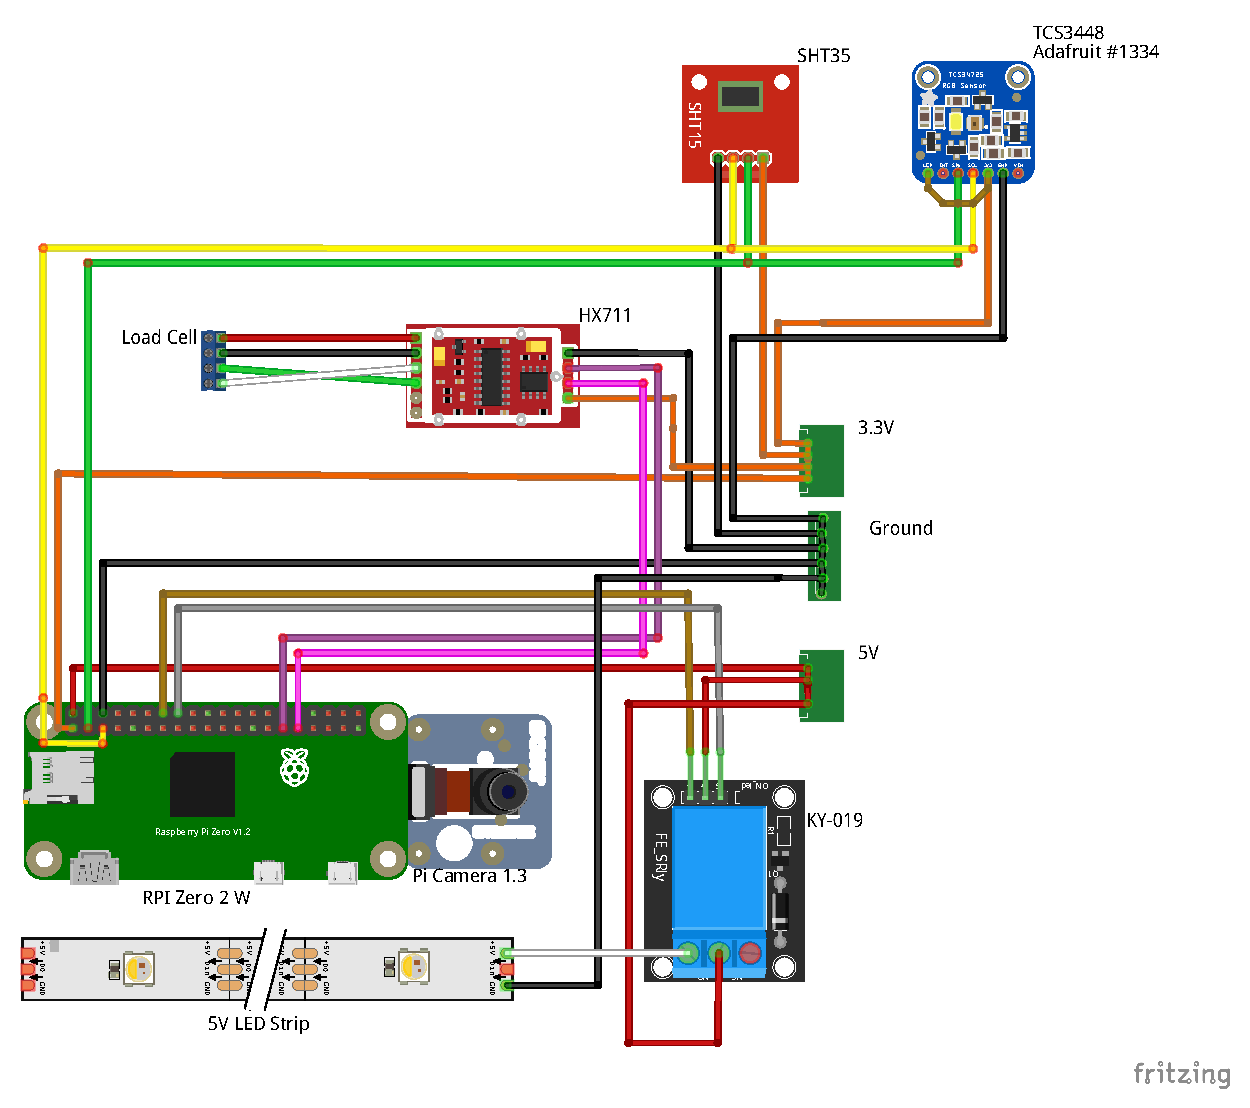
\includegraphics[width=0.95\textwidth]{Images/Wiring_Diagram.pdf}
\caption[PhenoHive Electronic Wiring Schematic]{Complete electronic schematic of the PhenoHive edge sensor station. The Raspberry Pi Zero 2~W is the central compute unit, connected to the SHT35 and TCS3448 over a shared I$^2$C bus, the load cell via an HX711 ADC, the LED relay on GPIO~23 (BCM), and the camera via CSI.}
\label{fig:wiring-schematic}
\end{figure}


\section{3D Printed Casing}
\label{sec:appendix-casing}

The PhenoHive station is housed in a custom designed casing made in CAD and fabricated with a standard 3D printer (Figure~\ref{fig:casing}). The design is available in the project repository under \texttt{casing/}.

The casing is a single continuously printed box with rounded outer corners and four insert holes at the corners for a lid attachment. The interior floor and sides have dedicated mounting pads for each electronic component.


\begin{figure}[H]
    \centering
    \begin{subfigure}[b]{0.52\textwidth}
        \centering
        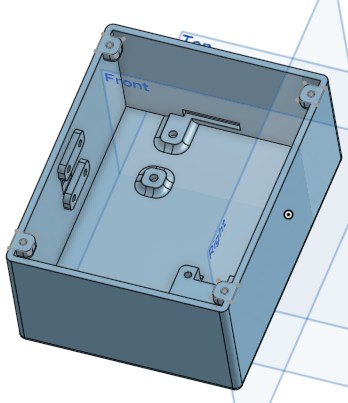
\includegraphics[width=\textwidth]{Images/3d_casing_isometric}
        \caption{Isometric CAD render showing the open-top enclosure, the camera bracket (left wall), and the circular TCS3448 sensor mount on the floor.}
        \label{fig:casing-isometric}
    \end{subfigure}
    \hfill
    \begin{subfigure}[b]{0.44\textwidth}
        \centering
        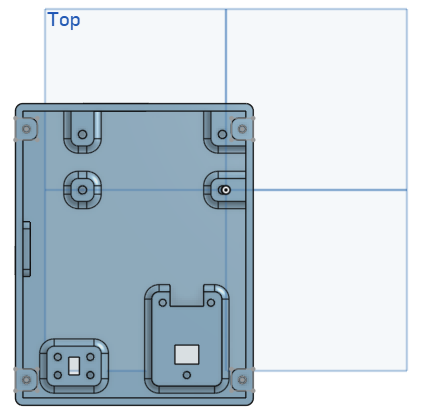
\includegraphics[width=\textwidth]{Images/3d_casing_top}
        \caption{Top-down view that shows the corner screw bosses, the circular sensor seat, the cable routing slot and the breakout board pad.}
        \label{fig:casing-top}
    \end{subfigure}
    \caption[PhenoHive 3D Printed Casing]{CAD renders of the PhenoHive 3D-printed casing. The design enforces a fixed sensor geometry across all stations. All of thefeatures are dimensioned to match the breakout boards listed in the bill of materials (Table~\ref{tab:bom}).}
    \label{fig:casing}
\end{figure}


\chapter{Bill of materials and cost analysis}
\label{ch:appendix-bom}

A primary objective of the PhenoHive project is maintaining a strict hardware budget to allow multi-station laboratory deployments (20+ units). The components were selected to balance precision with cost-efficiency. Table~\ref{tab:bom} details the pricing and sourcing of all components required to build one edge station. By using standard I$^2$C sensors and a Raspberry Pi Zero 2~W, the total hardware cost stays well within the 100--150€ target.


\begin{table}[htbp]
\centering
\caption[Bill of Materials for One PhenoHive Station]{Bill of Materials (BOM) for a single PhenoHive edge sensor station.}
\label{tab:bom}
\small
\renewcommand{\arraystretch}{1.2}
\begin{tabularx}{\textwidth}{|X|p{4cm}|r|}
\hline
\textbf{Component Description} & \textbf{Supplier} & \textbf{Approx. Cost (€)} \\
\hline
Raspberry Pi Zero 2~W with pre-soldered headers & Standard Retailer & 18.00 \\
\hline
Raspberry Pi Camera Module V1.3 (5MP) & Standard Retailer & 15.00 \\
\hline
MicroSD Card (32GB, Class 10) & Standard Retailer & 8.00 \\
\hline
Micro USB Power Supply (5V, 3A) & Standard Retailer & 10.00 \\
\hline
SHT35 Temperature \& Humidity Sensor Breakout & Adafruit / Seeed & 15.00 \\
\hline
TCS3448 Spectral Sensor (MikroE Color 21 Click) & MikroElektronika & 30.00 \\
\hline
TAL226 Load Cell (or equivalent generic strain gauge) & Generic Retailer & 10.00 \\
\hline
HX711 24-bit ADC Breakout Board & SparkFun / Generic & 2.00 \\
\hline
AZDelivery KY-019 Single-Channel Relay Module (5\,V) & AZDelivery / Generic & 3.00 \\
\hline
Luktix 5\,V COB USB LED Strip (1.5\,m, 4000\,K) & Generic Retailer & 8.00 \\
\hline
Wago 221-415 Splicing Connectors (for power distribution) & Hardware Store & 3.00 \\
\hline
Prototyping wires and 3D printed chassis & Local fabrication & 15.00 \\
\hline
\textbf{Total Estimated Cost} & & \textbf{$\approx$ 137.00} \\
\hline
\end{tabularx}

\end{table}


\chapter{Project repository}
\label{ch:appendix-repository}

The complete source code for this thesis is publicly available on GitHub:

\begin{center}
  \url{https://github.com/amontariol/Phenohive_2025-26}
\end{center}

The repository contains the full station software, deployment scripts, calibration tools, Grafana provisioning scripts, and the \LaTeX{} source for this report. It is archived under \textcite{phenohive-repo}.



\chapter{Station Assembly and Deployment Guide}
\label{ch:appendix-deployment-guide}

This appendix is a step-by-step reference for a TA or developer who needs to build and commission a new PhenoHive station from scratch. It covers hardware assembly, image build, and first-boot verification. The UCLouvain server-side infrastructure (InfluxDB, Grafana, auto-provisioning) is assumed to already be running; a brief setup reference is included at the end.

\section{Prerequisites}

Before starting, the following items should be ready:
\begin{itemize}
    \item All components listed in the Bill of Materials (Appendix~\ref{ch:appendix-bom}).
    \item A microSD card reader.
    \item A Linux machine to build the golden image (the build script requires \texttt{losetup}, \texttt{chroot} and \texttt{qemu-user-static}).
    \item SSH access to the UCLouvain VM and an admin InfluxDB token.
    \item A Tailscale account with admin right and a reusable pre-auth key generated from the Tailscale admin console.
    \item A 3D-printed enclosure (STL files in \texttt{docs/casing/} of the repository).
    \item The PhenoHive repository cloned locally.
\end{itemize}

\section{Hardware assembly}

Wire the components following the schematic in Figure~\ref{fig:wiring-schematic} (Appendix~\ref{sec:appendix-wiring}). The key connections are summarised below.

\begin{itemize}
    \item \textbf{SHT35 and TCS3448} both share the I$^2$C bus on GPIO~2 (SDA) and GPIO~3 (SCL). They both run at 3.3\,V.
    \item \textbf{HX711 ADC} DOUT on GPIO~5, PD\_SCK on GPIO~6 and the breakout is powered at 3.3\,V.
    \item \textbf{KY-019 relay} (LED strip control) DATA goes on GPIO~23 (BCM numbering) and is powered at 5\,V.
    \item \textbf{Camera module}: connected via the CSI ribbon cable to the Raspberry Pi Zero~2~W.
    \item \textbf{Power input}: a 5\,V / 3\,A Micro-USB power supply to the Raspberry Pi micro-USB power port.
\end{itemize}

Use Wago connectors to distribute the 3.3\,V, 5\,V and GND rails cleanly without needing to solder anything. All breakout boards can be set on their mounting pads and then close the enclosure lid.

\section{Prepare configuration and build the image}

All station-specific values are integrated into the image at build time. This means that no SD card editing or SSH access is required after flashing.

\paragraph{Create the configuration files} In the \texttt{dietpi/} directory of the repository, create three plain-text files (one value per file, no trailing whitespace):

\begin{center}
\begin{tabular}{|l|l|}
\hline
\textbf{File} & \textbf{Content} \\
\hline
\texttt{dietpi/phenohive\_server.txt} & Tailscale IP of the UCLouvain VM (e.g.\ \texttt{100.117.27.12}) \\
\texttt{dietpi/phenohive\_token.txt} & InfluxDB write token \emph{(gitignored --- do not commit)} \\
\texttt{dietpi/phenohive\_station\_id.txt} & Unique station identifier (e.g.\ \texttt{01}, \texttt{02}) \\
\hline
\end{tabular}
\end{center}

The build script reads these files and writes the values directly into \texttt{/opt/phenohive/.env} and \texttt{config.ini} inside the image.

\paragraph{Requirements} The build script (\texttt{dietpi/build\_image.sh}) requires a Linux host with:
\begin{itemize}
    \item \texttt{qemu-user-static} and \texttt{binfmt} support (for cross-architecture chroot).
    \item Standard utilities: \texttt{losetup}, \texttt{parted}, \texttt{e2fsck}, \texttt{resize2fs}, \texttt{rsync}.
    \item Internet access from within the chroot (for \texttt{apt-get} and the Tailscale repository).
\end{itemize}

\paragraph{Obtain the base image} Download the latest DietPi ARMv8 image for Raspberry Pi Zero~2~W from \url{https://dietpi.com/} and place it in the \texttt{dietpi/} directory. The script auto-detects any \texttt{DietPi*.img.xz} file there.

\paragraph{Run the build} From the repository root:
\begin{verbatim}
sudo ./dietpi/build_image.sh --tailscale-key tskey-auth-XXXXX
\end{verbatim}

Pass a reusable pre-auth key from the Tailscale admin console. The script performs the following steps inside a chroot of the base image:
\begin{enumerate}
    \item Installs the system packages: NetworkManager, comitup (captive-portal Wi-Fi onboarding), Tailscale, \texttt{python3-picamera2}, I$^2$C tools and Avahi.
    \item Enables \texttt{NetworkManager}, \texttt{comitup}, \texttt{avahi-daemon}, \texttt{tailscaled} and \texttt{phenohive} all as systemd services.
    \item Bakes the PhenoHive source tree into \texttt{/opt/phenohive/}, creates a Python virtual environment and installs all dependencies.
    \item Writes \texttt{.env} with the server IP and token read from the local configuration files, and \texttt{config.ini} with the station ID.
    \item Embeds the Tailscale pre-auth key for automatic first-boot authentication.
    \item Enables I$^2$C and the camera module via \texttt{config.txt} overlays and configures a fully unattended DietPi first boot.
\end{enumerate}

The output is called \texttt{dietpi/phenohive.img}, is approximately 5\,GB larger than the base image and build time is 20--40 minutes depending on network speed and host CPU.

\section{Flash the image}

Flash \texttt{dietpi/phenohive.img} to the microSD card. On Windows use Raspberry Pi Imager or Balena Etcher. On Linux:
\begin{verbatim}
dd if=dietpi/phenohive.img of=/dev/sdX bs=4M status=progress
\end{verbatim}

Insert the card into the Raspberry Pi and power it on. No further preparation of the SD card is needed.

\section{Wi-Fi setup via comitup}

Because no Wi-Fi credentials are stored in the image, the station cannot reach any network on first boot. The comitup service handles this automatically.

\begin{enumerate}
    \item Power on the station. After approximately 30 seconds, a Wi-Fi hotspot named \texttt{comitup-XXXX} appears (where XXXX is derived from the device MAC address).
    \item On a phone or laptop, connect to that hotspot. A captive portal opens automatically. If it does not, open a browser and navigate to \texttt{http://comitup.local}.
    \item Select the target Wi-Fi network from the list, enter the password and confirm. The hotspot disappears and the station joins the network.
    \item The station reboots automatically. On the second boot it authenticates to Tailscale using the baked-in key and the PhenoHive service starts.
\end{enumerate}

\textbf{Subsequent network changes:} if the station cannot find its saved network, comitup automatically re-broadcasts the hotspot. Repeat steps 2--3 to re-configure.

\section{Verify the service}

Once the station is on the network and Tailscale is authenticated, confirm the service is running. 
There are two ways to do this. You can either check the logs directly on the Pi via SSH, or monitor the incoming data on Grafana or the debug UI (next step).

To SSH into the Pi (via its Tailscale IP, available in the Tailscale admin console):

\begin{verbatim}
ssh root@<PI_TAILSCALE_IP>
Ctrl+C to stop the live log stream.
systemctl status phenohive
journalctl -u phenohive -n 60 --no-pager
\end{verbatim}

The log should show:
\begin{itemize}
    \item Sensor initialisation messages (\texttt{SHT35 OK}, \texttt{TCS3448 OK}, etc.).
    \item An NTP clock synchronisation confirmation.
    \item A \texttt{Collection cycle started} line after the first collection interval.
    \item A \texttt{Publishing aggregate record} line after the first publish interval.
\end{itemize}

If a sensor fails to initialise, the service continues and retries on every subsequent poll cycle. Check the wiring against Figure~\ref{fig:wiring-schematic} if a sensor does not recover.

If the service cannot reach the server, check:
\begin{itemize}
    \item \texttt{tailscale status} where both the VM and the station should appear as connected.
    \item \texttt{/opt/phenohive/.env} verify \texttt{INFLUX\_URL} and \texttt{INFLUX\_TOKEN} were applied correctly.
    \item That the provisioning files were placed on \texttt{/boot} before the first boot (they are only processed once, if this wasn't done, then reflash the compiled image to the sd card, there is no need to rebuild it entirely).
\end{itemize}

\section{Scale and Camera calibration}

Open the debug dashboard from any device on the same Tailscale network:

\begin{verbatim}
http://<PI_TAILSCALE_IP>:8080
\end{verbatim}

Navigate to the \emph{Calibration} tab to perform both the calibrations:

For the scale:
\begin{enumerate}
    \item Place the station on its final surface. Do not put anything on the scale and click on \emph{Confirm: Scale is empty}.
    \item Place an object with a known mass on the scale, then enter that mass in the \emph{Reference weight (g)} field and click \emph{Calibrate}. The reading should now match the reference.
    \item You can choose to add an offset correction to the calibration to take the pot's weight into account.
    \item Remove the calibration weight and place the plant (pot and soil) on the scale. Confirm the reading is plausible.
\end{enumerate}

For the camera:
\begin{enumerate}
    \item Ensure that the station is in its final position and the camera has a clear view of where the plant will be but without the plant in the frame and click on \emph{Capture background}. 
    \item Use an item in the captured image to compute the pixel-to-cm scale factor then enter the real-world size in cm and it's value in pixels on the image and click \emph{Calibrate}. The computed scale factor is applied to all subsequent recordings and is written to \texttt{config.ini}.
    
\end{enumerate}   
    This captures the current view as Calibration values (\texttt{tare} and \texttt{calibration\_factor}) are written to \texttt{config.ini} immediately and persist across reboots and software updates.

\section{Verify data on Grafana}

Within a few minutes of the first successful data push, the auto-provisioning service on the VM detects the new \texttt{station\_id} tag in InfluxDB and automatically creates:
\begin{itemize}
    \item A Grafana team (\texttt{phenohive\_station\_XX}).
    \item A student user account (\texttt{studentXX}) with an initial password derived from the station ID.
    \item A dashboard cloned from the master template and filtered to this station.
\end{itemize}

Log in to Grafana at \texttt{http://100.117.27.12:3000} as \texttt{usr: admin \& pwd: admin12345} and confirm the new dashboard appears. Share the student credentials (\texttt{studentXX} / \texttt{phenohive\_XX}) with the corresponding group.

\section{Optional: setting up the server-side infrastructure}

If the backend stack is not yet running (e.g.\ deploying a new course edition), set it up as follows.

\begin{enumerate}
    \item SSH into the VM and clone the repository.
    \item Copy \texttt{.env.example} to \texttt{.env} and set \texttt{INFLUXDB\_INIT\_ADMIN\_TOKEN}, \texttt{GRAFANA\_ADMIN\_PASSWORD} and \texttt{INFLUXDB\_INIT\_PASSWORD}.
    \item Start the production Docker stack:
    \begin{verbatim}
docker compose up -d
    \end{verbatim}
    \item Create a scoped InfluxDB write token (append-only to the \texttt{phenohive} bucket) via the InfluxDB web UI on port 8086 (accessible locally on the VM). This is the token that goes into \texttt{phenohive\_token.txt} on each station's SD card.
    \item Start the auto-provisioning service:
    \begin{verbatim}
python scripts/auto_provision_grafana.py
    \end{verbatim}
    Register it as a systemd unit for persistence across VM reboots.
    \item Install Tailscale on the VM and join the PhenoHive tailnet:
    \begin{verbatim}
tailscale up --auth-key=<TSKEY-AUTH-...>
    \end{verbatim}
\end{enumerate}

Once the VM stack is running, return to Step~2 to build and flash stations.

\chapter{Use of artificial intelligence tools}
\label{ch:appendix-ai}

In accordance with UCLouvain's policy on the use of generative artificial intelligence and academic transparency standards, the following AI tools were used during the development of this Master's thesis for the following purposes:
\begin{itemize}
    \item \textbf{Code assistance and debugging - Claude Code:} Was used as a pair-programming assistant throughout development to accelerate the writing of acquisition scripts and boilerplate code, to help debug I$^2$C driver issues and to help propose fixes to implementation problems. All of the suggested code was reviewed and tested on the physical hardware and was manually validated before integration into the codebase.
    \item \textbf{Mathematical assistance - Claude:} Was used to verify the calibration offset calculations and check various mathematical formulas. All results were independently and manually checked.
    \item \textbf{LaTeX formatting - Claude Code:} Was used to generate TikZ diagram scaffolding and tabular structure templates as well as general formatting assistance. All generated markup was reviewed, fact checked and adapted to match the thesis content.
    \item \textbf{Writing and proofreading - Claude:} Was used to correct grammar and spelling errors and to improve general clarity. All of the text in this manuscript reflects my own analysis, methodology and conclusions. There are no AI-generated passages that appear word-for-word in the final manuscript that weren't reviewed and revised.
\end{itemize}
All AI-assisted contributions were reviewed, tested where applicable and validated to ensure technical accuracy and scientific integrity.


\printbibliography[heading=bibintoc, title={References}]

\backcoverpage
\end{document}
